\chapter{Learning Fast Generators from Scratch}\label{ch:fast-scratch}

\epigraph{
    \textit{Truth is ever to be found in simplicity, and not in the multiplicity and confusion of things.
}}{Isaac Newton}


In \Cref{ch:distillation}, we saw that slow iterative samplers in diffusion models can be compressed into few-step generators through distillation. From an engineering perspective, two-stage pipelines are practical because they divide a complex generative training task into clear, independent objectives. The first stage learns the data distribution, while the second accelerates sampling or enhances quality. This separation allows each stage to be optimized independently, making the overall system easier to manage, more stable, and more reliable.

In this chapter, however, the focus shifts to a central question driving the progress of deep generative modeling:
\begin{question}
    Can we design a standalone generative principle that trains in a stable and efficient way, fast sampling, and allows users to easily guide or control what is produced?
\end{question}
In this chapter we pursue this direction and discuss an alternative approach:
training few-step diffusion-based generators \emph{without} relying on a pre-trained model.
Our focus is the \emph{flow-map model}. Here, a \emph{flow map} is the
classical solution map of an ODE, a notion rooted in differential
equations and dynamical systems and closely connected, in continuum and
fluid mechanics, to following the motion of material particles.
Specifically, $\bPsi_{s\to t}$ takes a state at time $s$ to the state
reached at time $t$ under the prescribed dynamics. A flow-map model
learns to approximate this map directly, allowing a long trajectory to
be traversed in one or a few network evaluations%
\footnote{See \Cref{eq:flow-map-def} and the surrounding discussion for
the mathematical and historical background of flow maps.}.
% \[
% \bPsi_{s\to t}(\rvx_s)
% =\rvx_s+\int_s^t \rvv^{*}(\rvx_u,u)\,\mathrm d u,
% \]
% where $\rvv^{*}$ denotes the target velocity field defined under the prescribed data-to-noise forward process
% $p_t(\cdot|\rvx_0)=\mathcal{N}(\cdot;\alpha_t\rvx_0,\sigma_t^2\rmI)$ with $\rvx_0\sim p_{\mathrm{data}}$.
This formulation provides a principled way to transport probability mass from the prior distribution $p_{\mathrm{prior}}$ to the data distribution $p_{\mathrm{data}}$,
while preserving the marginal distributions $p_t$ specified by the forward diffusion process at each intermediate time.


\chapterlearning{

  \item distinguish an instantaneous velocity field from its ODE solution map (flow map);

  \item understand the semigroup property of exact ODE flows and how it motivates consistency-based learning objectives;

  \item understand Consistency Model, Consistency Trajectory Model, and Mean Flow as representative ways to learn special or general flow maps;

  \item distinguish oracle flow-map identities from their practical approximations, and understand how suitable parametrizations enable few-step generation while retaining access to local velocity information.

}{The central object in this chapter is the ODE flow map. The individual methods should be viewed as different parametrizations and training strategies for learning this same underlying object.}

\newpage
\section{Prologue}

\begin{figure}[th]
  \centering
  \resizebox{0.95\linewidth}{!}{%
    \begin{tikzpicture}[x=2.6cm,y=1cm,line cap=butt]
      \tikzset{>={Stealth[length=12pt,width=16pt]}}
      \def\DotR{3pt}
      \def\LabelAngle{45}
      \def\DateAbove{4pt}
      \def\TextBelow{16pt}
      \newcommand{\nl}{\\}

      % Axis
      \draw[ultra thick,-Stealth] (0,0) -- (6.5,0);

      % IMPORTANT: no trailing comma on the last item
      \foreach \x/\date/\desc in {
        0.5/{2021/01}/{{\color{PersA}{KD}}\nl{\color{PersA}{Section~\ref{sec:distillation-prologue}}}},
        1.6/{2022/02}/{{\color{PersA}{PD}}\nl{\color{PersA}{Section~\ref{sec:PD}}}},
        2.7/{2023/03}/{{\color{PersA}{CM}}\nl{\color{PersA}{Section~\ref{sec:discrete-cm}}}},
        3.8/{2023/10}/{{\color{PersB}{CTM}}\nl{\color{PersB}{Section~\ref{sec:CTM}}}},
        4.9/{2024/10}/{{\color{PersA}{sCM}}\nl{\color{PersA}{Section~\ref{sec:conti-cm}}}},
        6.0/{2025/05}/{{\color{PersB}{MF}}\nl{\color{PersB}{Section~\ref{sec:MF}}}}% <-- NO COMMA HERE
      }{
        % dot
        \fill[black] (\x,0) circle[radius=\DotR];
        % date above
        \node[above=\DateAbove,align=center] at (\x,0) { \date};
        % text below (use shortstack; \nl expands to \$
        \node[below=\TextBelow,anchor=north,rotate=\LabelAngle,inner sep=1pt] at (\x,0)
          {\shortstack[c]{\strut \desc}};
      }
    \end{tikzpicture}%
  }
\caption{\textbfs{Timeline of diffusion-based methods for learning flow
maps.}\;
The underlying flow map is the classical ODE solution map; the dates
shown here refer only to modern machine-learning methods that distill,
approximate, or learn this map. We use {\color{PersA}blue} for the
special case {\color{PersA}$\bPsi_{s\to 0}$} and
{\color{PersB}orange} for the general map
{\color{PersB}$\bPsi_{s\to t}$}.
\figcredit{Created by the authors.}}
  \label{fig:timeline}
\end{figure}




\paragraph{Motivation of Flow Map Models.}
In \Cref{ch:distillation} we showed how the inaccessible regression target in the oracle flow-map loss
$\mathcal{L}_{\mathrm{oracle}}(\btheta)$ (see \Cref{eq:general-cm-loss:rep})
can be estimated by distilling knowledge from a pre-trained diffusion model to obtain few-step generators.
This route is effective and practical: a two-stage pipeline can be engineered for robustness
and often remains competitive in both data and compute efficiency.

In this chapter, we shift focus to a broader challenge at the core of deep generative modeling:
\emph{Can we establish a standalone generative principle that enables stable, scalable, and efficient training,
fast sampling, and generation that can be easily steered by user intentions, without relying on a pre-trained model?}
Designing such standalone principles lies at the center of generative modeling.

Diffusion models offer a useful design principle: start with a continuous-time forward process that gradually transforms data into a simple prior (noise) as a reference, and frame the modeling task as learning the reverse-time transport that restores this process to match the desired marginal distributions.  
This time-dependent formulation also makes it easier to steer the generation process at intermediate steps, compared to one-shot generative maps.  
Specializing to diffusion-motivated methods, this leads to the question:
\begin{question}
Can we learn the flow map $\bPsi_{s\to t}(\cdot)$ with a network
$\rmG_\btheta(\cdot,s,t)$ (a \emph{flow map model}) without access to pre-trained models,
while maintaining high-fidelity generation?
\end{question}
\begin{figure}[th!]
    \centering
    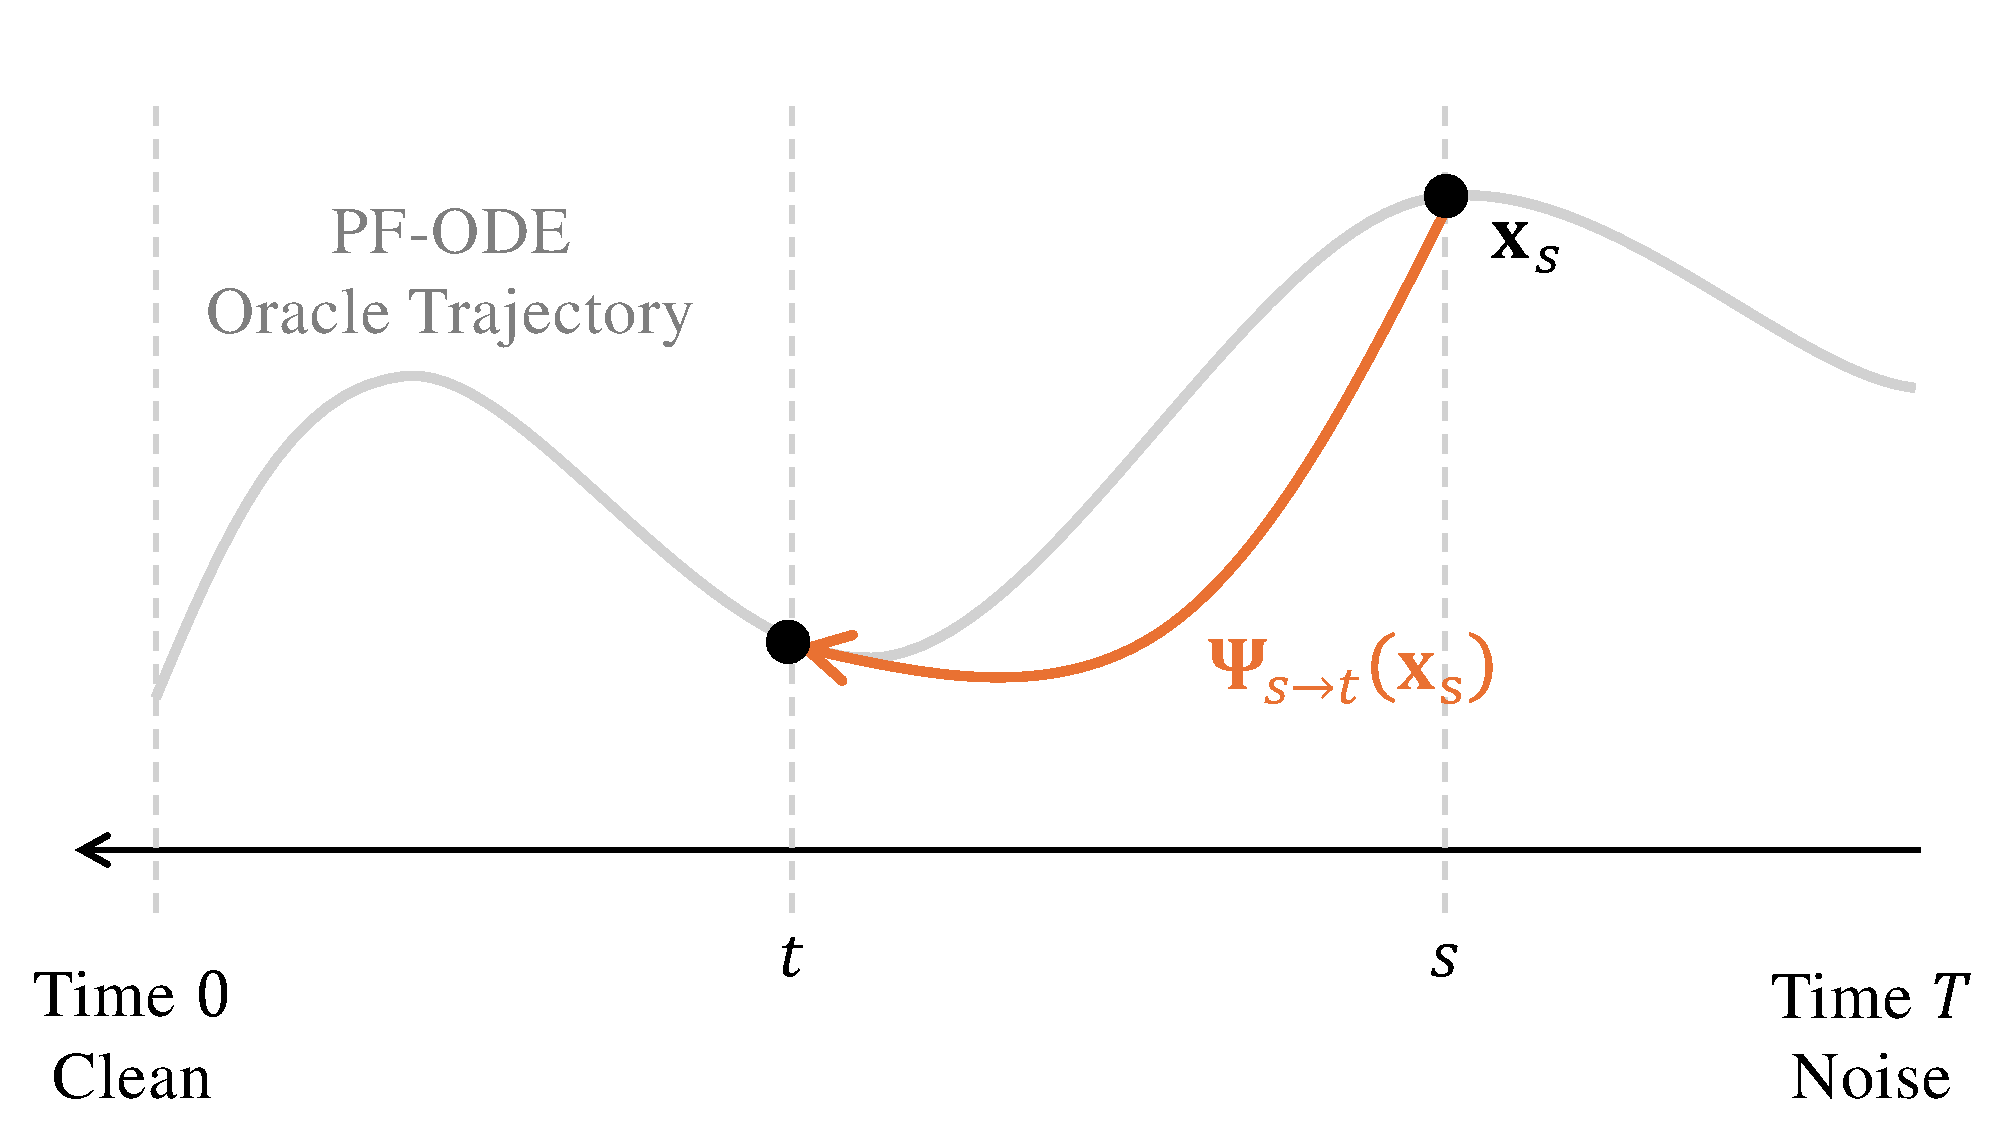
\includegraphics[width=0.9\linewidth]{Images/PartD/flow-map.pdf}
    \caption{\textbfs{Illustration of the flow map.} Starting from any state $\rvx_s$ at time $s$, 
the flow map $\bPsi_{s \to t}$ transports it to the corresponding point on the same PF-ODE oracle trajectory at time $t$. \figcredit{Created by the authors.}}
    \label{fig:flow-map-illustration}
\end{figure}


This chapter develops methods toward this goal, organized around a single objective
that also underlies distillation and provides a unified view of flow-map formulations~\citep{boffi2024flow,hu2025cmt}:
\begin{mdframed}
\begin{equation}\tag{\ref*{eq:general-cm-loss}}\label{eq:general-cm-loss:rep}
  \mathcal{L}_{\mathrm{oracle}}(\btheta)
  := \mathbb{E}_{s,t}\,\mathbb{E}_{\rvx_s \sim p_s}\Big[
     w(s,t)  d\big(\rmG_\btheta(\rvx_s,s,t),  \bPsi_{s\to t}(\rvx_s)\big)
  \Big].
\end{equation}
\end{mdframed}


% Optional: do not consume a new equation number
\addtocounter{equation}{-1}
Here $s,t$ are sampled from some time distribution (e.g., uniform),
$w(s,t) \ge 0$ assigns weights to the time pairs $(s,t)$, and $d(\cdot,\cdot)$
is a discrepancy measure such as the squared $\ell_2$ norm. The oracle flow map
$\bPsi_{s\to t}$ represents the ideal transformation that takes a state
$\rvx_s$ at time $s$ and transports it directly to time $t$:
\[
\bPsi_{s\to t}(\rvx_s) = \rvx_s + \int_s^t \rvv^*(\rvx_u,u)\,\mathrm{d}u,
\]
where the oracle drift is given as
\[
\rvv^*(\rvx_u,u) = \E \left[\alpha_u'\rvx_0+ \sigma_u'\beps | \rvx_u\right],
\]
while equivalent parametrizations are also possible  (see \Cref{ch:all-equivalent}), with common choices including the $\rvx$-prediction and $\rvv$-prediction forms. 

At the optimum of the oracle loss, the learned model recovers the true flow map
exactly:
\[
\rmG^*(\rvx_s, s, t) = \bPsi_{s\to t}(\rvx_s), \quad \text{for all }\, s,t, \text{ and }\, \rvx_s \sim p_s.
\]


Because the flow map $\bPsi_{s\to t}$ cannot be expressed in closed form, it must be approximated. 
One option, discussed in \Cref{ch:distillation}, is to rely on a pre-trained diffusion model. 
Alternatively, as we will see in this chapter, new and more tractable surrogates can be introduced. 
For clarity, existing approaches can be broadly categorized according to whether the training procedure queries a teacher during the loop: 
\emph{distillation}, which explicitly calls a teacher model, and 
\emph{training from scratch}, which avoids teacher calls by constructing self-contained surrogates.



Building on this principled
objective, we now turn to systematic approaches for learning flow map models,
with the aim of developing methods that are practical while also producing
generations that more accurately reflect the true data distribution and are
computationally efficient. We begin with a high-level introduction to this paradigm.
\paragraph{Special Flow Map: Consistency Functions.}
\emph{Consistency Models}~\citep{song2023consistency} represent one of the earliest pioneering approaches to flow-map learning. 
They learn a few-step denoiser $\rvf_\btheta(\cdot,s)$ that approximates the special case of the flow map to the origin:
\[
\bPsi_{s\to 0}(\cdot), \qquad s \in (0,T].
\]
The key idea is that every state $\rvx_s$ is mapped to the time-$0$ endpoint
$\bPsi_{s\to 0}(\rvx_s)$ of the PF-ODE trajectory passing through it. Formally, the oracle training objective for the CM family~\citep{song2023consistency,songimproved,geng2024consistency,lu2024simplifying} is
\begin{align}\label{eq:oracle-cm}
    \mathcal{L}_{\methodl{oracle}{CM}}(\btheta) 
    := \E_{s} \E_{\rvx_s\sim p_s} \left[ w(s)  d \left(\rvf_\btheta(\rvx_s,s), \bPsi_{s\to 0}(\rvx_s)\right)\right].
\end{align}




In practice, however, the oracle $\bPsi_{s\to 0}(\rvx_s)$ is unavailable. It is therefore replaced by a \emph{stop-gradient} target, denoted as $\rvf_{\btheta^-}$, taken from a slightly earlier step $\bPsi_{s\to s-\Delta s}(\rvx_s)$ on the same trajectory:
\[
\bPsi_{s\to 0}(\rvx_s) \approx \rvf_{\btheta^-} \left(\bPsi_{s\to s-\Delta s}(\rvx_s),\,s-\Delta s\right), \quad \Delta s > 0,
\]
where $\bPsi_{s\to s-\Delta s}(\rvx_s)$ itself must also be approximated. Two
practical strategies are available: (i) \emph{distillation}, which relies on a
pre-trained diffusion model, and (ii) \emph{training from scratch}, which uses a
one-point estimate without teacher guidance.

% \begin{itemize}
%     \item \textbfs{Distillation:} use a one-step solver applied to a pre-trained diffusion model. This approach is called \emph{Consistency Distillation (CD)}.
%     \item \textbfs{From Scratch:} use the analytic one-point estimate
%     \[
%       \rvx_{s-\Delta s} = \alpha_{s-\Delta s}\,\rvx_0 + \sigma_{s-\Delta s}\,\beps,
%     \]
%     with the same $(\rvx_0,\beps)$ as in $\rvx_s = \alpha_s \rvx_0 + \sigma_s \beps$. This approach is called \emph{Consistency Training (CT)}.
% \end{itemize} 


\paragraph{General Flow Map.} Two representative approaches are the \emph{Consistency Trajectory Model} (CTM) and \emph{Mean Flow} (MF).
\subparagraph{Consistency Trajectory Models.} \emph{Consistency Trajectory Model} (CTM)\\~\citep{kim2023consistency} is the first work to learn the general flow map $\bPsi_{s\to t}$ for arbitrary start and end times, and can be viewed as a concrete instance under the unified objective of \Cref{eq:general-cm-loss:rep}. CTM adopts an Euler-inspired parametrization by expressing the oracle flow map as
\begin{align*}
\bPsi_{s\to t}(\rvx_s)
:= \rvx_s + \int_s^t \rvv^*(\rvx_u,u)\diff u 
= \frac{t}{s} \rvx_s
+ \frac{s-t}{s}
\underbrace{\Big[\rvx_s + \frac{s}{s-t} \int_s^t \rvv^*(\rvx_u,u) \diff u\Big]}_{\approx~\rvg_{\btheta}},
\end{align*}
which motivates the neural parameterization
\[
\rmG_{\btheta}(\rvx_s,s,t)
:= \frac{t}{s}\,\rvx_s + \frac{s-t}{s}\,\rvg_\btheta(\rvx_s,s,t),
\]
where $\rvg_\btheta$ is a neural network trained so that $\bPsi_{s\to t}(\rvx_s)\approx \rmG_{\btheta}(\rvx_s,s,t)$.

Since the oracle $\bPsi_{s\to t}(\rvx_s)$ is inaccessible, CTM trains against a \emph{stop-gradient} target evaluated at an intermediate time $u$:
\[
\bPsi_{s\to t}(\rvx_s)
 \approx 
\rmG_{\btheta^-} \big(\bPsi_{s\to u}(\rvx_s),\,u,\,t\big),
\qquad u\in[t,s],
\]
where the intermediate state $\bPsi_{s\to u}(\rvx_s)$ is approximated in one of
two ways: (i) \emph{distillation}, which uses a few-step solver applied to a
pre-trained diffusion teacher, or (ii) \emph{training from scratch}, which
constructs a self-induced teacher directly through the $\rmG_\btheta$
parametrization.


\subparagraph{Mean Flow.}
Mean Flow (MF)~\citep{geng2025mean} builds on flow matching by modeling the \emph{average drift} over an interval $[t,s]$ (with $t\le s$):
\[
\rvh_{\btheta}(\rvx_s,s,t)
 \approx 
\rvh^*(\rvx_s,s,t)
:= \frac{1}{\,t-s\,}\int_s^t \rvv^*(\rvx_u,u)\,\diff u,
\]
also aligning with \Cref{eq:general-cm-loss:rep}.
Differentiating the identity
\[
(t-s)\,\rvh^*(\rvx_s,s,t)  =  \int_s^t \rvv^*(\rvx_u,u)\,\diff u
\]
with respect to $s$ yields a self-referential relation that motivates the MF objective
\[
\mathcal{L}_{\mathrm{MF}}(\btheta)
:= \E_s\,\E_{\rvx_s\sim p_s} \Big[w(s)\,\big\|
\rvh_{\btheta}(\rvx_s,s,t)-\rvh_{\btheta^-}^{\mathrm{tgt}}(\rvx_s,s,t)
\big\|_2^2\Big],
\]
with stop-gradient target
\[
\rvh_{\btheta^-}^{\mathrm{tgt}}(\rvx_s,s,t)
:= \rvv^*(\rvx_s,s)  -  (s-t) \left((\partial_\rvx \rvh_{\btheta^-})\,\rvv^*(\rvx_s,s) + \partial_s \rvh_{\btheta^-}\right).
\]
In practice, the oracle velocity $\rvv^*(\rvx_s,s)$ must also be approximated.
Two common strategies are: (i) \emph{distillation}, which leverages a
pre-trained diffusion model trained with flow matching, or (ii) \emph{training
from scratch}, which uses the one-point conditional velocity
$\alpha'_s\,\rvx_0+\sigma'_s\,\beps$ derived from the forward corruption process
$\rvx_s = \alpha_s \rvx_0+\sigma_s \beps$.



\subparagraph{Relationship Between CTM and MF.}
CTM and MF approximate the same path integral but parameterize different surrogates of it:
\begin{align*}
\bPsi_{s\to t}(\rvx_s)
&:= \rvx_s  +  \int_s^t \rvv^*(\rvx_u,u)\,\diff u
\\[2pt]
&= \frac{t}{s}\,\rvx_s
 +  \frac{s-t}{s}\,
\underbrace{\Big[\rvx_s + \frac{s}{\,s-t\,} \int_s^t \rvv^*(\rvx_u,u)\,\diff u\Big]}_{\approx~\rvg_{\btheta} }
\\[4pt]
&= \rvx_s  +  (t-s)\,
\underbrace{\Big[\frac{1}{\,t-s\,} \int_s^t \rvv^*(\rvx_u,u)\,\diff u\Big]}_{\approx~\rvh_{\btheta} }.
\end{align*}
In words, CTM learns an \emph{slope displacement} through $\rvg_\btheta$, while MF learns the \emph{average drift} $\rvh_\btheta$; both are consistent ways to approximate the same integral that defines $\bPsi_{s\to t}$.


\paragraph{What Happens Next?}
We begin with the CM family, which focuses on the specific flow map
$\bPsi_{s\to 0}$. This part covers both its discrete time origin in
\Cref{sec:discrete-cm} and its continuous time extension in
\Cref{sec:conti-cm}. We then move on to the general flow map and provide a
detailed discussion of two key representatives, CTM and MF. Their
parameterizations, training strategies, and practical approximations are
presented in \Cref{sec:CTM} and \Cref{sec:MF}, respectively.

We remark that the \emph{Elucidating Diffusion Model} (EDM) introduced in
\Cref{sec:edm} offers systematic guidelines for designing the network
parameterization of the $\rvx$-prediction model and has demonstrated strong
empirical performance. Although this section can be considered optional, the
EDM formulation serves as a valuable foundation for CM-style models.


For clarity of exposition later on, we do not strictly follow the chronological order in which these approaches appeared. 
Instead, we organize the discussion by conceptual relationships. 
Nevertheless, to acknowledge originality and respect chronology, we provide the historical timeline in \Cref{fig:timeline}.




%%%%%%%%%%%%%%%%%%%%%%%%


\clearpage
\newpage


\section{Special Flow Map: Consistency Model in Discrete Time}\label{sec:discrete-cm}

\paragraph{An Important Principle of Flow Maps: The Semigroup Property.}
\begin{figure}[th!]
    \centering
    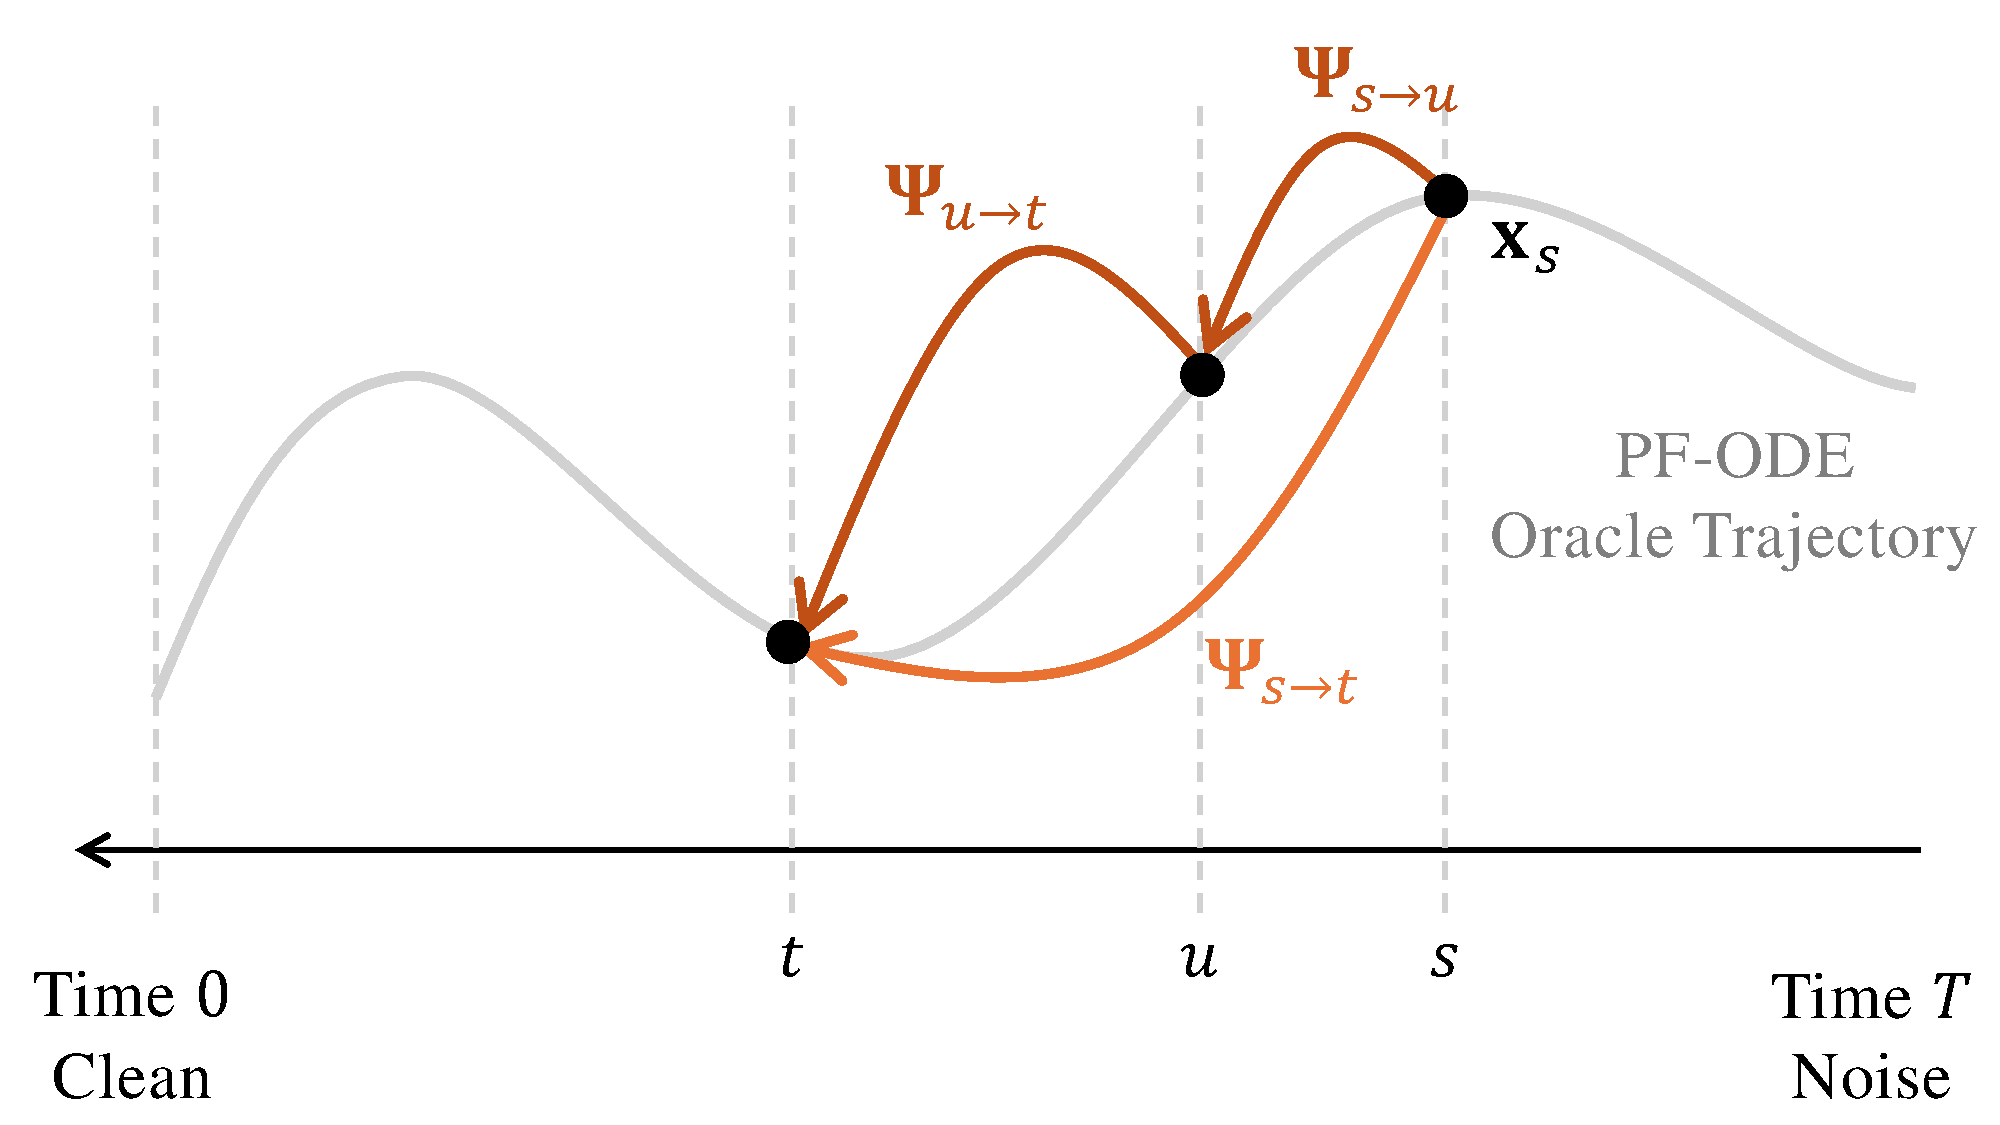
\includegraphics[width=0.9\linewidth]{Images/PartD/semigroup.pdf}
    \caption{\textbfs{Illustration of the flow map semigroup property.} 
This property states that transitioning from $s$ to $u$ and then from $u$ to $t$ 
is equivalent to transitioning directly from $s$ to $t$.
\figcredit{Created by the authors.}}
    \label{fig:semigroup}
\end{figure}


Consistency Models (introduced in \Cref{sec:discrete-cm,sec:conti-cm}) and their generalization, the Consistency Trajectory Model (\Cref{sec:CTM}), define their regression targets by exploiting a key mathematical structure of flow maps. 
This structure is the fundamental \emph{semigroup property}:
\begin{mdframed}
   \begin{align}\label{eq:semi-group}
       \bPsi_{u\to t}\circ \bPsi_{s\to u}=\bPsi_{s\to t},
       \,\,\,
       \bPsi_{s\to s}=\rmI, \quad \text{for all }\, s, u, t \in [0,T].
   \end{align} 
\end{mdframed}
Intuitively, this means that if we first evolve a state from $s$ to $u$ (through $\bPsi_{s\rightarrow u}$)  and then from $u$ to $t$ (through $\bPsi_{u\rightarrow t}$), we end up at exactly the same point as if we had evolved directly from $s$ to $t$. 
This is nothing more than the basic principle of ODE solving\footnote{The semigroup property follows from the uniqueness theorem for ODE initial value problems (see \Cref{app:de}).}: once the starting point of a flow is specified, its future evolution is completely determined, and it follows a single well-defined path. Whether we follow this path in one long step or divide it into smaller intervals, we still move along the same trajectory and arrive at the same final state.

To build further intuition for the semigroup property, consider the solution trajectory $\{\rvx(s)\}_{s \in [0,T]}$ of the PF-ODE
\begin{align*}
    \frac{\diff \rvx(\tau)}{\diff \tau} = \rvv^*(\rvx(\tau), \tau),
\end{align*}
with a fixed initial condition $\rvx(T)$ at time $T$, solved backward in time.  
If we fix the terminal time at $t=0$, the corresponding flow map can be written more simply as
\[
\rvf^*(\cdot, s) := \bPsi_{s\to 0}(\cdot),
\]
which is referred to as the \emph{consistency function}.  
By construction, this function inherits several fundamental properties directly from the semigroup identity of \Cref{eq:semi-group} with $t=0$:

\begin{enumerate}
    \item[(i)] \textbfs{Global Consistency:} every point along the trajectory maps to the same clean endpoint,
    \[
       \rvf^*(\rvx(s), s) = \rvx(0), \quad \text{for all }\, s \in [0,T].
    \]
    This is because 
\begin{align*}
\rvf^*(\rvx(s),s)
&= \bPsi_{s\to 0}\big(\bPsi_{0\to s}(\rvx(0))\big)
= \big(\bPsi_{s\to 0}\circ \bPsi_{0\to s}\big)(\rvx(0))
\\&= \bPsi_{0\to 0}(\rvx(0))
= \rvx(0).
\end{align*}
    \item[(ii)] \textbfs{Self Consistency:} any two points along the same trajectory must give identical outputs,
    \begin{align}\label{eq:cm-self-consistency}
       \rvf^*(\rvx(s), s) = \rvf^*(\rvx(u), u), \quad \text{for all }\, s, u \in [0,T].
    \end{align}
    This is a direct re-interpretation of the semigroup identity: $\Psi_{s\rightarrow 0}\circ\Psi_{0\rightarrow s}=\Psi_{u\rightarrow 0}\circ\Psi_{0\rightarrow u}$.
    \item[(iii)] \textbfs{Local Consistency:} the consistency function is invariant with respect to $s$ when evaluated along the trajectory,
    \begin{align}\label{eq:cm-diff}
        \frac{\diff}{\diff s}\,\rvf^*(\rvx(s),s) = 0,
        \qquad \rvf^*(\rvx(0),0) = \rvx(0).
    \end{align}
This follows from global consistency, which states that $\rvf^*(\rvx(s), s)$ does
not change with $s$ along the trajectory.
\end{enumerate}
The three properties are all equivalent. Each states that along any solution trajectory $s\mapsto \rvx(s)$,
the flow-to-origin/consistency map $\rvf^*(\rvx(s),s)=\bPsi_{s\to 0}(\rvx(s))$
yields the same terminal point $\rvx(0)$, independent of the starting time.


\paragraph{Goal of Consistency Models.}
A CM aims to train a neural network 
$\rvf_{\bm{\theta}} \colon \mathbb{R}^D \times [0,T] \to \mathbb{R}^D$ 
to approximate the special flow map $\bPsi_{s\to 0}$, i.e., consistency function\footnote{The concept of a consistency function for an ODE generalizes to a function
$\rvf(\rvx,t)$ for an SDE such that $\rvf(\rvx_t,t)$ is a (local) martingale with
respect to the SDE’s natural filtration, i.e.
\[
\E[\rvf(\rvx_t,t)|\rvx_s]=\rvf(\rvx_s,s),\quad\text{for all }\quad t\ge s.
\]
This generalization was proposed/observed in \citep{daras2023consistent,lai2023fp},
and the theoretical connections are summarized in \citep{lai2023equivalence}.}. 
The key idea is to enforce consistency along PF-ODE trajectories: states lying
on the same ODE trajectory should map to the same time-$0$ endpoint
(more precisely, this corresponds to the special case $t=0$ and
$u=s-\Delta s$ in \Cref{eq:semi-group}).

There are, however, multiple ways to realize this goal. 
The choice depends on whether a pre-trained diffusion model is available and whether training is carried out in a discrete-time or continuous-time regime. 
We begin by summarizing these variants in \Cref{tb:consistency-methods} and illustrating their objectives in \Cref{fig:cd-ct-loss-distill}. 
The subsequent sections (\Cref{sec:discrete-cm,sec:conti-cm}) then gradually develop the details of each approach.

\begin{table}[th]
  \caption{Training Objectives of Consistency Models}
  \small
  \centering
  \resizebox{0.76\textwidth}{!}{
  \begin{tabular}{ccc}
     \toprule
     & \textbfs{Distillation} & \textbfs{From Scratch} \\
     \midrule
     \textbfs{Discrete-time} & \Cref{eq:cd-discrete-approx-N} & \Cref{eq:ct-discrete-approx-N} \\
     \textbfs{Continuous-time} & \Cref{eq:cd-continuous-time}  & \Cref{eq:ct-continuous-time} \\
     \bottomrule
  \end{tabular}
  }
  \label{tb:consistency-methods}
\end{table} 




\subsection{Discrete-Time Approximations for Learning a Consistency Function}\label{subsec:approx-cm}

In principle, a consistency function can be learned by minimizing the oracle loss \Cref{eq:oracle-cm}:
\[
    \mathcal{L}_{\methodl{oracle}{CM}}(\btheta) 
    := \E_{s} \E_{\rvx_s\sim p_s} \left[ w(s)  d \left(\rvf_\btheta(\rvx_s,s), \bPsi_{s\to 0}(\rvx_s)\right)\right].
\]
This objective enforces that every noisy sample $\rvx_s$ is mapped back to its clean endpoint $\bPsi_{s\to 0}(\rvx_s)$.  

The challenge is that the oracle map $\bPsi_{s\to 0}(\rvx_s)$ is not available in practice.  
To overcome this, \citet{song2023consistency} exploit the \emph{semigroup property}: any noisy state and its consecutive step along the same PF-ODE trajectory must map to the same clean endpoint.  
Concretely, the oracle target is replaced by a \emph{stop-gradient} target taken from a slightly earlier point on the trajectory:
\begin{align*}
    \bPsi_{s\to 0}(\rvx_s) 
    &= \bPsi_{s-\Delta s \to 0} \left(\bPsi_{s\to s-\Delta s}(\rvx_s)\right) \\
    &\approx \rvf_{\btheta^-} \left(\bPsi_{s\to s-\Delta s}(\rvx_s),\,s-\Delta s\right), 
    \qquad \Delta s > 0,
\end{align*}
where $\bm{\theta}^-$ are parameters under the stop-gradient operator. 
A further difficulty is that the intermediate state $\bPsi_{s\to s-\Delta s}(\rvx_s)$ has no closed form either and must itself be approximated.  
Two practical regimes have been proposed:

\paragraph{With Pre-trained Diffusion Model (Consistency Distillation).}
Suppose we have access to a pre-trained diffusion model. 
Consistency Distillation (CD) leverages the teacher model to approximate the intermediate state $\bPsi_{s\to s-\Delta s}(\rvx_s)$ by simulating only a single backward ODE step:
\[
 \bPsi_{s\to s-\Delta s}(\rvx_s)  \approx  \mathtt{Solver}_{s \to s-\Delta s}(\rvx_s).
\]

More concretely, a pre-trained diffusion model provides an estimate of the score function 
$\rvs_{\bm{\phi}^\times}(\rvx_s, s) \approx \nabla_{\rvx_s}\log p_s(\rvx_s)$. 
Using this, one can perform a one-step DDIM update from $\rvx_s$ to obtain an approximation of the state at $s' = s-\Delta s$:
\begin{align*}
    \bPsi_{s\to s-\Delta s}(\rvx_s) 
    &\approx \frac{\alpha_{s'}}{\alpha_s}\,\rvx_s 
    + \sigma_s^2 \left( \frac{\alpha_{s'}}{\alpha_s} - \frac{\sigma_{s'}}{\sigma_s} \right)\nabla_{\rvx_s}\log p_s(\rvx_s) \\
    &\approx \frac{\alpha_{s'}}{\alpha_s}\,\rvx_s 
    + \sigma_s^2 \left( \frac{\alpha_{s'}}{\alpha_s} - \frac{\sigma_{s'}}{\sigma_s} \right)\rvs_{\bm{\phi}^\times}(\rvx_s, s) \\
    &:= \tilde{\rvx}_{s'}^{\bm{\phi}^\times}.
\end{align*}

Combining this construction with the stop-gradient target yields a practical \emph{discrete-time} proxy for the oracle loss $\mathcal{L}_{\methodl{oracle}{CM}}(\btheta)$. 
Formally, over a partition $0 = s_1 < s_2 < \cdots < s_N = T$, the CD training objective is given by
\begin{mdframed}
\begin{align}\label{eq:cd-discrete-approx-N}
    \mathcal{L}_{\text{CD}}^N(\bm{\theta}, \bm{\theta}^-; \bm{\phi}^\times) 
    := \E_{\rvx_0, \beps, i} \Big[\, \omega(s_i)\,
    d\big(\rvf_{\bm{\theta}}(\rvx_{s_{i+1}}, s_{i+1}),\, 
          \rvf_{\bm{\theta}^-}(\tilde{\rvx}_{s_i}^{\bm{\phi}^\times}, s_i)\big)\Big].
\end{align}
\end{mdframed}
Here, $\omega(\cdot)$ is a time-dependent weight, $d(\cdot,\cdot)$ is a distance measurement, and $\bm{\theta}^-$ indicates stop-gradient parameters, which prevent collapse to trivial solutions (e.g., constant predictions).


    
\paragraph{Without Pre-Trained Diffusion Model (Consistency Training).}
When no pre-trained diffusion model is available, the oracle score $\nabla_{\rvx}\log p_s(\rvx_s)$ can still be estimated directly using a simple one-point approximation (albeit with high variance). 
Recall that it admits the conditional expectation form:
\begin{align*}
    \nabla_{\rvx_s} \log p_s(\rvx_s)
    &= \E_{\rvx_0 \sim p(\rvx_0|\rvx_s)} \left[ \nabla_{\rvx_s}\log p(\rvx_s|\rvx_0) \right] \\
    &= \E_{\rvx_0 \sim p(\rvx_0|\rvx_s)} \left[ -\frac{\rvx_s - \alpha_s \rvx_0}{\sigma_s^2} \right].
\end{align*}
The identity above suggests a simple one-sample estimator. 
If $\rvx_s$ is obtained from a paired sample $(\rvx_0,\beps)$ via $\rvx_s = \alpha_s \rvx_0 + \sigma_s \beps$, then 
\[
\widehat{\nabla_{\rvx}\log p_s}(\rvx_s)
:=-\frac{\boldsymbol\epsilon}{\sigma_s}
=-\frac{\rvx_s-\alpha_s \rvx_0}{\sigma_s^2}
\]
serves as an \emph{unbiased} estimator of the score at $\rvx_s$ (conditionally unbiased with respect to $p(\rvx_0|\rvx_s)$). It corresponds exactly to the \emph{conditional score} used as the regression target in denoising score matching.



Plugging this estimate into the DDIM one-step update from $s$ to $s' = s-\Delta s$ (see \Cref{eq:ddim-update-all}) yields
\begin{align}\label{eq:one-pt-score}
\begin{aligned}
    \bPsi_{s\to s'}(\rvx_s)
&\approx
\frac{\alpha_{s'}}{\alpha_s}\,\rvx_s 
+ \sigma_s^2 \left(\frac{\alpha_{s'}}{\alpha_s}-\frac{\sigma_{s'}}{\sigma_s}\right)\nabla_{\rvx_s}\log p_s(\rvx_s) && \text{(DDIM)}
\\
&\approx
\frac{\alpha_{s'}}{\alpha_s}\,\rvx_s 
+ \sigma_s^2 \left(\frac{\alpha_{s'}}{\alpha_s}-\frac{\sigma_{s'}}{\sigma_s}\right)\widehat{\nabla_{\rvx_s}\log p_s}(\rvx_s) && \text{(1-pt score)}
\\
&=
\frac{\alpha_{s'}}{\alpha_s}\,\rvx_s 
-\left(\frac{\alpha_{s'}}{\alpha_s}-\frac{\sigma_{s'}}{\sigma_s}\right)(\rvx_s-\alpha_s\rvx_0)
\\
&= \alpha_{s'}\rvx_0+\sigma_{s'}\beps, 
\end{aligned}
\end{align}
where\footnote{The last identity follows directly from the forward corruption process $\rvx_s=\alpha_s \rvx_0+\sigma_s \beps$ by elementary algebra.}
$\rvx_0$ is the same data sample and $\beps$ is the same Gaussian noise used to
construct $\rvx_s$.


This leads to a teacher-free discrete-time surrogate of the oracle objective $\mathcal{L}_{\methodl{oracle}{CM}}$, written as
\begin{mdframed}
\begin{align}\label{eq:ct-discrete-approx-N}
    \mathcal{L}_{\text{CT}}^N(\bm{\theta}, \bm{\theta}^-) 
    := \E_{\rvx_0, \beps, i} \left[ 
       \omega(s_i)\, d \left(\rvf_{\bm{\theta}}(\rvx_{s_{i+1}}, s_{i+1}),\, 
       \rvf_{\bm{\theta}^-}(\rvx_{s_i}, s_i)\right)
    \right],
\end{align}
\end{mdframed}
with $\rvx_{s_i} = \alpha_{s_i}\rvx_0 + \sigma_{s_i}\beps$ and $\rvx_{s_{i+1}} = \alpha_{s_{i+1}}\rvx_0 + \sigma_{s_{i+1}}\beps$.

Using $\alpha_{s'}\rvx_0+\sigma_{s'}\beps$ directly as an approximation of $\bPsi_{s\to s'}(\rvx_s)$ without expectation introduces high variance\footnote{The one-point (conditional) score estimate $\widehat{\nabla_{\rvx}\log}p_s(\rvx_s)$ can be viewed as a one-sample Monte Carlo estimator, which is \emph{conditionally unbiased} given $\rvx_s$: averaging this estimator over the (generally intractable) clean posterior $p(\cdot|\rvx_s)$ recovers the true score as
\[
\nabla_{\rvx_s}\log p_s(\rvx_s)
= \E_{\rvx_0\sim p(\cdot|\rvx_s)}
 \left[\widehat{\nabla_{\rvx}\log}p_s(\rvx_s)\right].
\]}. 
Recall, however, the analogous conditional-expectation argument in denoising
score matching (see \Cref{sec:conditional-trick}). Here, the one-point state
estimate is unbiased before it is passed through the nonlinear target network
and discrepancy, so the resulting losses need not agree exactly. Conditioning
on $\rvx_s$, the first-order error cancels in expectation; under suitable
smoothness and moment assumptions, the remaining discrepancy is
$\mathcal{O}(\Delta s^2)$, as formalized below.

% The one-point (conditional) score estimate $\widehat{\nabla_{\rvx}\log}p_s(\rvx_s)$ can be viewed as a one-sample Monte Carlo estimator, which is \emph{conditionally unbiased} given $\rvx_s$: averaging this estimator over the (generally intractable) clean posterior $p(\cdot|\rvx_s)$ recovers the true score as
% \[
% \nabla_{\rvx_s}\log p_s(\rvx_s)
% = \E_{\rvx_0\sim p(\cdot|\rvx_s)}
%  \left[\widehat{\nabla_{\rvx}\log}p_s(\rvx_s)\right].
% \]
% If one uses $\alpha_{s'}\rvx_0+\sigma_{s'}\beps$ directly as an approximation of $\bPsi_{s\to s'}(\rvx_s)$ without expectation generally yields high variance. 
% However, after taking the full expectation in the loss (Theorem~\ref{thm:ct-cm}), this one-sample estimator remains unbiased; hence, the one-point score approximation is justified at the loss level.
% In this sense, the update below serves as a practical approximation to the DDIM step computed with an oracle score.
% The following theorem formalizes this expectation-level justification of the one-point estimator.

% and hence,
% \begin{align}
% \begin{aligned}
%     \bPsi_{s\to s'}(\rvx_s)
% &\approx
% \frac{\alpha_{s'}}{\alpha_s}\,\rvx_s 
% + \sigma_s^2 \left(\frac{\alpha_{s'}}{\alpha_s}-\frac{\sigma_{s'}}{\sigma_s}\right)\nabla_{\rvx_s}\log p_s(\rvx_s) && \text{(DDIM)}
% \\
% &=
% \frac{\alpha_{s'}}{\alpha_s}\,\rvx_s 
% + \sigma_s^2 \left(\frac{\alpha_{s'}}{\alpha_s}-\frac{\sigma_{s'}}{\sigma_s}\right) \E_{\rvx_0\sim p(\cdot|\rvx_s)}
%  \left[\widehat{\nabla_{\rvx}\log}p_s(\rvx_s)\right] 
% \\
% &=
% \frac{\alpha_{s'}}{\alpha_s}\,\rvx_s 
% -\left(\frac{\alpha_{s'}}{\alpha_s}-\frac{\sigma_{s'}}{\sigma_s}\right)(\rvx_s-\alpha_s\rvx_0)
% \\
% &=  \E_{\rvx_0\sim p(\cdot|\rvx_s)}
%  \left[\rvx_0+\sigma_{s'}\beps\right]\alpha_{s'}=:\hat\rvx_{s'}, 
% \end{aligned}
% \end{align}




\thmp{CM-CT Equivalence up to Error $\mathcal{O}(\Delta s^2)$}{ct-cm}{
Let $s' := s - \Delta s$, and define
\begin{align*}
\mathcal{L}_{\mathrm{CM}}(\btheta,\btheta^-)
&:= \E_{s,\rvx_0,\beps} \big[w(s)\,d\big(\rvf_{\btheta}(\rvx_s,s), \rvf_{\btheta^-}(\rvx_{s'}^{\mathrm{DDIM}},s')\big)\big],\\
\mathcal{L}_{\mathrm{CT}}(\btheta,\btheta^-)
&:= \E_{s,\rvx_0,\beps} \big[w(s) d\big(\rvf_{\btheta}(\rvx_s,s), \rvf_{\btheta^-}(\rvx_{s'},s')\big)\big],
\end{align*}
where
\[
\rvx_{s'}^{\mathrm{DDIM}}
:= \frac{\alpha_{s'}}{\alpha_s}\rvx_s
+ \sigma_s^2 \left(\frac{\alpha_{s'}}{\alpha_s}-\frac{\sigma_{s'}}{\sigma_s}\right)\nabla_{\rvx_s}\log p_s(\rvx_s)
\]
is the oracle DDIM update.  Both  $\rvx_s = \alpha_s\rvx_0 + \sigma_s\beps$  and $\rvx_{s'} = \alpha_{s'}\rvx_0 + \sigma_{s'}\beps$
share the same pair $(\rvx_0,\beps)$ with 
$\rvx_0 \sim p_{\mathrm{data}}$ and 
$\beps \sim \mathcal{N}(\bm{0},\rmI)$.
Then,
\[
\mathcal{L}_{\mathrm{CM}}(\btheta,\btheta^-)
= \mathcal{L}_{\mathrm{CT}}(\btheta,\btheta^-) + \mathcal{O}(\Delta s^2).
\]
}{First, note that the DDIM update with the oracle score equals the conditional mean,
\[
\rvx_{s'}^{\mathrm{DDIM}} = \E[\rvx_{s'} | \rvx_s],
\]
which can also be verified from \Cref{eq:one-pt-score} by taking the expectation over $p(\cdot|\rvx_s)$.
Next, perform a Taylor expansion of
\[
d(\rvf_{\btheta}(\rvx_s,s), \rvf_{\btheta^-}(\cdot,s'))
\]
around
$\rvx_{s'}^{\mathrm{DDIM}}=\E[\rvx_{s'}|\rvx_s]$.
The one-point update recovers
$\rvx_{s'}=\alpha_{s'}\rvx_0+\sigma_{s'}\beps$ pathwise for the same
$(\rvx_0,\beps)$. Since
\[
\E[\rvx_{s'}-\rvx_{s'}^{\mathrm{DDIM}}\mid\rvx_s]=0,
\]
the linear Taylor term vanishes after conditioning on $\rvx_s$.
Under the smoothness and moment assumptions described above, the remaining
expected Taylor remainder is $\mathcal{O}(\Delta s^2)$. Hence,
$\mathcal{L}_{\mathrm{CT}}
=\mathcal{L}_{\mathrm{CM}}+\mathcal{O}(\Delta s^2)$.
A detailed derivation is provided in \Cref{app-sec:flow-map}.
}

In summary, CD leverages a teacher model for initialization and supervision, which often stabilizes optimization and reduces variance.  In contrast, Consistency Training (CT) requires no pre-trained model and can therefore be trained entirely from scratch.
Despite this difference, CT serves as a fully standalone generative model.
\paragraph{Practical Considerations.}
In practice, \citet{song2023consistency} adopt the EDM formulation
of \citet{karras2022elucidating} (see \Cref{sec:edm}) with the forward corruption
kernel $    \rvx_s = \rvx_0 + s \bm{\epsilon}$, and use the neural network parameterization proposed therein
(cf.\ \Cref{eq:D-parametrization}):
\[
    \rvf_{\bm{\theta}}(\rvx, s)
    = c_{\mathrm{skip}}(s) \rvx
      + c_{\mathrm{out}}(s)\,
        \rmF_{\bm{\theta}} \left(c_{\mathrm{in}}(s)\,\rvx,\, c_{\mathrm{noise}}(s)\right),
\]
where $\rmF_{\bm{\theta}}$ is a neural network and the coefficients follow
\Cref{eq:edm-simple-coefficients}. This parameterization has the important
boundary property
\[
    \rvf_{\bm{\theta}}(\rvx, 0) = \rvx,
\]
which enforces consistency at time zero and ensures the network output matches
its input when no noise is present.





% Assume that $\rvf_{\bm{\theta}}$ learns the optimal trajectory defined by the empirical PF-ODE of the teacher model as in \Cref{eq:teacher-pf-ode}. We revisit \Cref{eq:conti-ct-motivation}  when staying on a trajectory $\{\bar\rvx(s)\}_{s\in[0, T]}$ of the empirical ODE: 
% \begin{align*}
%         &\rvf_{\bm{\theta}^*}(\bar\rvx(s), s) \equiv \bar\rvx(0), \quad \text{for all } s\in [0,T]
%         \\
%         \Leftrightarrow~&\left(\nabla_{\rvx} \rvf_{\bm{\theta}^*}\right)(\bar\rvx(s), s) \cdot 
%     \underbrace{\frac{\diff }{\diff s} \bar\rvx(s)}_{\text{ODE velocity}} + 
%     \left(\frac{\partial }{\partial s} \rvf_{\bm{\theta}^*}\right)(\bar\rvx(s), s) \equiv 0\\
%         \Leftrightarrow~&\left(\nabla_{\rvx} \rvf_{\bm{\theta}^*}\right)(\bar\rvx(s), s) \cdot \rvv_{\bm{\phi}^\times}(\bar\rvx(s), s) + \left(\frac{\partial }{\partial s} \rvf_{\bm{\theta}^*}\right)(\bar\rvx(s), s) \equiv 0
%     \end{align*}

\subsection{Sampling with Consistency Model}\label{subsec:cm-sampling}
Once a consistency model $\rvf_{\bm{\theta}^\times}$ is trained, either in continuous or discrete time, it can be used to generate samples in a single step or a few steps. The algorithm is summarized in \Cref{alg:cm_sampling}.

\paragraph{One-Step Generation.} Given an initial latent $\hat{\rvx}_T$ sampled from the prior distribution (in practice,  $\mathcal{N}(\bm{0}, T^2\rmI)$), a clean sample can be generated via a single function evaluation: $\rvf_{\bm{\theta}^\times}(\hat{\rvx}_T, T)$.

\paragraph{Multi-Step Generation.} With pre-selected timesteps 
$T>\tau_1 > \tau_2 > \cdots > \tau_{M-1}=0$, start from initial noise $\hat\rvx_T$ and alternate between noise injection and large clean jumps via the consistency model at earlier time points, gradually refining the sample:
\begin{align*}
    \hat\rvx_T \xrightarrow[\text{get a clean}]{\text{long jump}} \rvf_{\bm{\theta}^\times}(\hat\rvx_T, T)
    \xrightarrow[\text{to level $\tau_1$}]{\text{add noise}} \hat\rvx_{\tau_1}
    \xrightarrow[\text{get a clean}]{\text{long jump}} \rvf_{\bm{\theta}^\times}(\hat\rvx_{\tau_1}, \tau_1)
    \xrightarrow[\text{to level $\tau_2$}]{\text{add noise}} \cdots.
\end{align*}

\begin{algorithm}[thb!]
    {\small
        \caption{CM's Sampling with One-Step or Multi-Step Generation \label{alg:cm_sampling}}
    \begin{algorithmic}[1]
        \Require Consistency model $\rvf_{\bm{\theta}^\times}(\cdot, \cdot)$, sequence of time points $T>\tau_1 > \tau_2 > \cdots > \tau_{M-1}=0$, initial noise $\hat{\rvx}_T$
        \If{one-step}
            \State $\rvx \leftarrow \rvf_{\bm{\theta}^\times}(\hat{\rvx}_T, T)$
        \Else
            \State $\rvx \leftarrow \rvf_{\bm{\theta}^\times}(\hat{\rvx}_T, T)$
            \For{$m=1$ \textbf{to} $M-1$}
                \State Sample $\bm{\epsilon} \sim \mathcal{N}(\bm{0}, \bfI)$
                \State $\hat{\rvx}_{\tau_m} \leftarrow \alpha_{\tau_m}\rvx + \sigma_{\tau_m} \bm{\epsilon}$
                \State $\rvx \leftarrow \rvf_{\bm{\theta}^\times}(\hat{\rvx}_{\tau_m}, \tau_m)$
            \EndFor
        \EndIf
        \Ensure $\rvx$
    \end{algorithmic}
    }
\end{algorithm}














% \subsection{(Optional) Properties of Consistency Function}\label{subsec:consistency-function} 
% CM is motivated by fundamental properties of ODE solution maps, specifically the uniqueness of trajectories once the initial condition is fixed, a classical result from ODE theory.

% Let $\{\rvx(s)\}_{s \in [0, T]}$ denote the solution trajectory of the PF-ODE:
% \begin{align*}
%     \frac{\diff \rvx(\tau)}{\diff \tau} 
%     = f(\tau) \rvx(\tau) - \tfrac{1}{2}g^2(\tau) \nabla_\rvx \log p_\tau(\rvx(\tau)) 
%     =: \rvv^*(\rvx(\tau), \tau),
% \end{align*}
% with some fixed initial condition $\rvx(T)$ at time $T$, solved in reverse time. The oracle consistency function $\rvf^*(\rvx, s):=\bPsi_{s\to 0}(\rvx)$, defined as in \Cref{eq:int_target_gt}, satisfies the following key properties:
% \proppp{Properties of the Solution Map}{cm-sol-map}{
% \begin{enumerate}
%     \item \textbfs{Global Consistency}: $\rvf^*(\rvx(s), s)=\rvx(0)$, for all $s\in[0,T]$.
%     \item \textbfs{Self Consistency}: 
%   \begin{align}\label{eq:cm-self-consistency}
%           \rvf^*(\rvx(s), s)=\rvf^*(\rvx(s'), s'),\quad\text{for any } s, s' \in [0,T].
%   \end{align}
%     \item \textbfs{Local Consistency:}
%     \begin{align}\label{eq:cm-diff}
%         \frac{\diff }{\diff s} \rvf^*(\rvx(s), s) = 0 \quad \text{with} \quad \rvf^*(\rvx(0), 0) = \rvx(0).
%     \end{align}
% \end{enumerate}
% }{These properties directly follow from the semigroup property of the ODE (uniqueness theorem for ODE solutions, commonly known as the Picard-Lindel\"of or Carath\'eodory global existence and uniqueness theorem).}

% It is straightforward to verify that these three properties are actually equivalent. All of these conditions say that: along a given solution trajectory, the solution map yields the same terminal point regardless of the starting time.   


% \rmkb{The concept of a consistency function for an ODE generalizes to a function
% $\rvf(\rvx,t)$ for an SDE such that $\rvf(\rvx_t,t)$ is a (local) martingale with
% respect to the SDE’s natural filtration, i.e.
% \[
% \E[\rvf(\rvx_t,t)|\rvx_s]=\rvf(\rvx_s,s),\quad\text{for all }\quad t\ge s.
% \]
% This generalization was proposed/observed in \citep{daras2023consistent,lai2023fp},
% and the theoretical connections are summarized in \citep{lai2023equivalence}.
% }


% The three equivalent conditions discussed above suggest multiple ways to learn a consistency function. Consistency Models (CM)~\citep{song2023consistency} adopt the \emph{self-consistency property} of \Cref{eq:cm-self-consistency}, which requires that, for any inputs lying on the same ODE solution trajectory, the predicted clean data remains unchanged. We elaborate on this idea in the following subsection, focusing on the distillation-based variant, known as Consistency Distillation (CD).







\clearpage
\newpage

\section{Special Flow Map: Consistency Model in Continuous Time}\label{sec:conti-cm}

We now move beyond the discrete-time setting of consistency models and consider
a continuous-time perspective. Unlike the discrete approach, which fixes a time
grid and trains only on those sampled points, the continuous formulation treats
the flow map as defined for all times. This shift eliminates the dependence on
an arbitrary discretization and provides a more principled alignment with the
underlying dynamics. It also helps reduce the approximation errors that
naturally arise from discretized integration, and ensures consistency is
enforced globally rather than only at selected steps.

\subsection{Continuous-Time Consistency Model}\label{subsec:conti-ct}
To motivate the continuous time formulation, we first revisit
\Cref{eq:cm-diff}, which describes the condition under which time derivatives
can be taken. Using the chain rule, we arrive at
\begin{align}\label{eq:conti-ct-motivation}
\begin{aligned}
        &\frac{\diff }{\diff s} \rvf^*(\rvx(s), s) = 0 \\
    \Longleftrightarrow\,\, 
    &\left(\nabla_{\rvx} \rvf^*\right)(\rvx(s), s) \cdot 
    \underbrace{\frac{\diff }{\diff s} \rvx(s)}_{\text{ODE velocity}} + 
    \left(\frac{\partial }{\partial s} \rvf^*\right)(\rvx(s), s) = 0,
\end{aligned}
\end{align}
where the trajectory $\rvx(s)$ follows the PF-ODE
\begin{align*}
    \frac{\diff }{\diff s}\rvx(s) =  \rvv^*(\rvx(s), s).
\end{align*}

This relationship shows that the consistency function $\rvf^*$ remains constant
along any solution trajectory of the ODE. The velocity field $\rvv^*$ can be
estimated in practice either from a pre-trained diffusion model (when such a
model is available) or from a direct one-point approximation, such as
$\alpha_s' \rvx_0 + \sigma_s' \beps$, as explained in
\Cref{sec:discrete-cm}.  

\Cref{eq:conti-ct-motivation} suggests a natural continuous-time characterization of consistency along PF-ODE trajectories. One possible approach is to enforce this differential condition directly by minimizing the residual, in a manner similar to physics-informed neural networks (PINNs)~\citep{raissi2018deep,boffi2024flow}:
\begin{align*}
\min_{\bm{\theta}}
\mathbb{E}_{s,\rvx_s\sim p_s}
\left[
\left\|
\partial_s\rvf_{\bm{\theta}}(\rvx_s,s)
+
\big(\partial_{\rvx}\rvf_{\bm{\theta}}(\rvx_s,s)\big)
\rvv^*(\rvx_s,s)
\right\|_2^2
\right].
\end{align*}

In practice, however, \citet{song2023consistency,lu2024simplifying} employ teacher-based consistency objectives rather than directly optimizing this residual. This motivates asking whether the discrete consistency loss admits a meaningful infinitesimal counterpart as $\Delta s \to 0$. The proposition below shows that, at the comparison point where the stop-gradient target coincides with the online network, the scaled discrete-time gradient converges to the gradient of a continuous-time objective:
\begin{align}\label{eq:cm-discrete}
\mathcal{L}_{\mathrm{CM}}^{\Delta s}(\btheta,\btheta^-)
:= \E \left[\omega(s) \big\|
\rvf_{\btheta}(\rvx_s,s) -
\rvf_{\btheta^-} \big(\bPsi_{s\to s-\Delta s}(\rvx_s), s-\Delta s\big)
\big\|_2^2\right].
\end{align}
% Here, the short-time flow map $\bPsi_{s\to s-\Delta s}(\rvx_s)$ can be
% approximated either with the help of a pre-trained diffusion model
% (i.e., distillation setting) or by a simple one point estimate
% (i.e., training from scratch). 
For a uniform partition underlying
\Cref{eq:cd-discrete-approx-N,eq:ct-discrete-approx-N}, let
\[
\Delta s_N:=\frac{T}{N-1}.
\]
Then $\Delta s_N\to0$ as $N\to\infty$, so the infinitesimal limit in
\Cref{eq:cm-discrete} corresponds to refining these discrete objectives.
 

We summarize this key idea in the following proposition.


\proppp{Continuous-Time Consistency Training}{continuous-time-ct}{The following convergence result holds at $\bm{\theta}=\bm{\theta}^-$:
\begin{align*}
    \left.\lim_{\Delta s\to 0}\frac{1}{\Delta s}\nabla_{\btheta}\mathcal{L}_{\mathrm{CM}}^{\Delta s}(\bm{\theta}, \bm{\theta}^-)\right|_{\bm{\theta}=\bm{\theta}^-}
    =
    \left.\nabla_{\bm{\theta}} \mathcal{L}^\infty_{\mathrm{CM}}(\bm{\theta}, \bm{\theta}^-)\right|_{\bm{\theta}=\bm{\theta}^-}.
\end{align*}
Here,
\begin{align*}
    \mathcal{L}^\infty_{\mathrm{CM}}(\bm{\theta},\bm{\theta}^-)
    :=
    \mathbb{E}_{s,\rvx_0,\bm{\epsilon}}\left[
    2\omega(s)\,
    \rvf_{\bm{\theta}}^\top(\rvx_s, s)\cdot
    \frac{\diff }{\diff s}\rvf_{\bm{\theta}^-}(\rvx_s, s)
    \right],
\end{align*}
and the total differentiation identity is
\begin{align}\label{eq:total-diff}
    \frac{\diff}{\diff s}\rvf_{\btheta^-}(\rvx_s,s)
    =
    \partial_s \rvf_{\btheta^-}(\rvx_s,s)
    + \big(\partial_{\rvx}\rvf_{\btheta^-}(\rvx_s,s)\big)\rvv^*(\rvx_s,s).
\end{align}
}{A first-order Taylor expansion of the stop-gradient target around $(\rvx_s, s)$ shows that the loss $\mathcal{L}_{\mathrm{CM}}^{\Delta s}$ behaves, up to $\mathcal{O}(\Delta s^2)$, like an inner product between the student update $\nabla_{\btheta}\rvf_{\btheta}(\rvx_s,s)$ and the tangent change $\tfrac{\diff}{\diff s}\rvf_{\btheta^-}(\rvx_s,s)$. Evaluating at $\bm{\theta}=\bm{\theta}^-$ removes the zeroth-order discrepancy term, so the scaled gradient satisfies
\[
\left.\lim_{\Delta s\to 0}\frac{1}{\Delta s}\nabla_{\btheta}\mathcal{L}_{\mathrm{CM}}^{\Delta s}\right|_{\bm{\theta}=\bm{\theta}^-}
=
\left.\nabla_{\btheta}\E\left[
2\omega(s)\,
\rvf_{\btheta}^\top(\rvx_s,s)\cdot
\frac{\diff}{\diff s}\rvf_{\btheta^-}(\rvx_s,s)
\right]\right|_{\bm{\theta}=\bm{\theta}^-},
\]
which is the claimed identity. We defer the proof to \Cref{app-sec:flow-map}.
}

The result above is written under the gradient operator
$\nabla_{\bm{\theta}}$ so that terms involving $\bm{\theta}^-$ vanish, since
$\bm{\theta}^-$ is treated as constant under stop-gradient.  Note
that $\tfrac{\diff}{\diff s}\rvf_{\btheta^-}(\rvx_s,s)$ denotes the total
derivative along the oracle trajectory, rather than a simple partial time
derivative.  

In summary, the continuous-time consistency model can be trained using the
gradient of the following pseudo-objective (ignoring the factor $2$):
\begin{mdframed}
    \begin{align}\label{eq:conti-ct-loss}
    \mathcal{L}^\infty_{\mathrm{CM}}(\bm{\theta},\bm{\theta}^-) := \mathbb{E}_{s,\rvx_0, \bm{\epsilon}}\left[\omega(s)\rvf_{\bm{\theta}}^\top(\rvx_s, s) \cdot \frac{\diff }{\diff s} \rvf_{\bm{\theta}^-}(\rvx_s, s) \right]. 
\end{align}
\end{mdframed}


\subsection{Training Continuous-Time Consistency Model}
Similar to the discrete-time case discussed in \Cref{subsec:approx-cm}, 
we now clarify the practical approximation of the tangent term in 
\Cref{eq:conti-ct-loss}, which involves the inaccessible oracle velocity $\rvv^*$:
\begin{align*}
    \frac{\diff}{\diff s}\rvf_{\btheta^-}(\rvx_s,s)
    = \partial_s \rvf_{\btheta^-}(\rvx_s,s)
    + \big(\partial_{\rvx}\rvf_{\btheta^-}(\rvx_s,s)\big)\,\rvv^*(\rvx_s,s).
\end{align*}
After training a continuous-time CM, sampling follows the same procedure as in
the discrete time case (\Cref{subsec:cm-sampling}).

\paragraph{Continuous-Time Consistency Distillation.}
If a pre-trained diffusion model is available such that
$\rvv_{\bm{\phi}^\times} \approx \rvv^*$, then the tangent vector
$\tfrac{\diff}{\diff s}\rvf_{\btheta^-}(\rvx_s,s)$ in
\Cref{eq:total-diff} can be approximated by the surrogate
\begin{align}\label{eq:cd-continuous-time}
    \frac{\diff}{\diff s}\rvf_{\btheta^-}(\rvx_s,s) 
     \approx 
    \partial_s \rvf_{\btheta^-}(\rvx_s,s)
    + \big(\partial_{\rvx}\rvf_{\btheta^-}(\rvx_s,s)\big)\,
      \rvv_{\bm{\phi}^\times}(\rvx_s,s).
\end{align}
We denote the resulting objective as
$\mathcal{L}^\infty_{\mathrm{CM}}(\bm{\theta},\bm{\theta}^-;\bm{\phi}^\times)$.
Accordingly, Proposition~\ref{continuous-time-ct} can be restated as
\[
\lim_{N\to\infty} 
\frac{1}{\Delta s_N}\,\nabla_{\bm{\theta}}\,
\mathcal{L}_{\mathrm{CD}}^{N}(\bm{\theta},\bm{\theta}^-;\bm{\phi}^\times)
= 
\nabla_{\bm{\theta}}\,
\mathcal{L}_{\mathrm{CD}}^{\infty}(\bm{\theta},\bm{\theta}^-;\bm{\phi}^\times).
\]


\paragraph{Continuous-Time Consistency Training (from Scratch).} On the other hand, if a pre-trained diffusion model is not available, the oracle
velocity $\rvv^*$ can be approximated using the one point conditional estimate
$\alpha_s'\rvx_0 + \sigma_s'\beps$. In this case, the tangent vector
$\tfrac{\diff}{\diff s}\rvf_{\btheta^-}(\rvx_s,s)$ in
\Cref{eq:total-diff} is replaced by the surrogate
\begin{align}\label{eq:ct-continuous-time}
    \frac{\diff}{\diff s}\rvf_{\btheta^-}(\rvx_s,s) 
     \approx 
    \partial_s \rvf_{\btheta^-}(\rvx_s,s)
    + \big(\partial_{\rvx}\rvf_{\btheta^-}(\rvx_s,s)\big) 
      \left(\alpha_s'\rvx_0 + \sigma_s'\beps\right).
\end{align}
We denote the resulting objective as
$\mathcal{L}^\infty_{\mathrm{CT}}(\bm{\theta},\bm{\theta}^-)$, which corresponds
to the training from scratch setting. Accordingly,
Proposition~\ref{continuous-time-ct} can be restated as
\[
\lim_{N\to\infty} 
\frac{1}{\Delta s_N}\,\nabla_{\bm{\theta}} 
\mathcal{L}_{\mathrm{CT}}^{N}(\bm{\theta},\bm{\theta}^-)
=
\nabla_{\bm{\theta}} 
\mathcal{L}_{\mathrm{CT}}^{\infty}(\bm{\theta},\bm{\theta}^-).
\]



So far, we have introduced all the fundamental approaches listed in 
\Cref{tb:consistency-methods} to realize the learning of the consistency 
function $\bPsi_{s\to 0}$. 
To provide a clearer overview, \Cref{fig:cd-ct-loss-distill} summarizes the 
relationships among the different loss functions for training consistency 
functions. 
The figure also indicates whether each method relies on a pre-trained diffusion 
model and distinguishes between continuous time and discrete time objectives.




\begin{figure}[ht]
\centering
\scalebox{0.9}{ 
\begin{tikzpicture}[
  box/.style={draw, rounded corners, thick, minimum width=3.5cm, minimum height=1cm, align=center},
  arrow/.style={thick, -{Latex[length=3mm]}},
  xshift=0cm, yshift=0cm
]

% Nodes
\node[box] (discCD) {\small{Discrete-Time CD}};
\node[box, right=4.5cm of discCD] (discCT) {\small{Discrete-Time CT}};
\node[box, below=2cm of discCD] (contCD) {\small{Continuous-Time CD}};
\node[box, below=2cm of discCT] (contCT) {\small{Continuous-Time CT}};

% Arrows with centered labels
\draw[arrow] (discCD) -- node[midway, above] {\footnotesize 
\shortstack{
$\mathcal{L}_{\text{CD}}(\bm{\theta},\bm{\theta}^-)  =\mathcal{L}_{\text{CT}}(\bm{\theta},\bm{\theta}^-) + \mathcal{O}(\Delta s^2)$
\\
\scriptsize (Theorem~\ref{thm:ct-cm})
}
} (discCT);
\draw[arrow] (discCD) -- node[midway, left] {
  \footnotesize
  \shortstack{
    $\displaystyle\lim_{N\rightarrow\infty} \frac{1}{\Delta s_N}\nabla_{\bm{\theta}}\mathcal{L}^N_{\text{CD}}$ \\ $=\nabla_{\bm{\theta}}\mathcal{L}^\infty_{\text{CD}}  $ \\
\scriptsize (Theorem 5)   
  }
} (contCD);
\draw[arrow] (discCT) -- node[midway, right] {
  \footnotesize
  \shortstack{
    $\displaystyle\lim_{N\rightarrow\infty} \frac{1}{\Delta s_N}\nabla_{\bm{\theta}}\mathcal{L}^N_{\text{CT}}  $\\
    $= \nabla_{\bm{\theta}}\mathcal{L}^\infty_{\text{CT}}$ \\
\scriptsize (Theorem 6) 
  }
} (contCT);
\draw[arrow] (discCD) to[out=-30,in=150] node[midway, above, yshift=-8.5mm, text width=5.2cm, align=center] {
  \footnotesize
  \shortstack{
    $\displaystyle\lim_{N\rightarrow\infty} \frac{1}{\Delta s_N}\nabla_{\bm{\theta}}\mathcal{L}^N_{\text{CD}}(\bm{\theta},\bm{\theta}^-;\bm{\phi}^\times)  $\\
    $= \nabla_{\bm{\theta}}\mathcal{L}^\infty_{\text{CT}}(\bm{\theta},\bm{\theta}^-)$ \\
\scriptsize (Theorem 6) 
  }
} (contCT);
\draw[arrow] (contCD) -- node[midway, below] {
  \footnotesize
  \shortstack{
    $\mathcal{L}^\infty_{\text{CD}}(\bm{\theta},\bm{\theta}^-;\bm{\phi}^\times)= \mathcal{L}^\infty_{\text{CT}}(\bm{\theta},\bm{\theta}^-)$ 
  }
} (contCT);
\end{tikzpicture}
}
\caption{\textbfs{Diagram showing relationships between discrete/continuous-time CD and CT under the $\ell_2$ distance metric: $d(\rvx,\rvy)=\|\rvx-\rvy\|_2^2$.} The marked theorems follow the labeling in \citep{song2023consistency}. Whenever the theorems involve CT, we assume a perfect score: $\rvs_{\bm{\phi}^\times}(\rvx, t) \equiv \nabla_\rvx \log p_t(\rvx)$. $\mathcal{L}^\infty_{\text{CT}}$ is defined in \Cref{eq:conti-ct-loss}, while $\mathcal{L}^\infty_{\text{CD}}$ is defined in \Cref{eq:cd-continuous-time}.
\figcredit{Created by the authors.}}
\label{fig:cd-ct-loss-distill}
\end{figure}



However, the tangent vector 
$\tfrac{\diff }{\diff s}\rvf_{\bm{\theta}^-}$ 
often causes instability during training. 
In the following optional section, we present techniques from 
\emph{Simplifying, Stabilizing and Scaling Continuous Time Consistency Models} 
(sCM)~\citep{lu2024simplifying} that mitigate these issues.





\subsection{(Optional) Practical Considerations of Continuous-Time CT} 
Our interest lies in the training from scratch scenario, since it yields a
standalone generative model that does not rely on external pre-trained diffusion
models. Hence, we focus our discussion on the continuous time case.

In practice, however, training directly with \Cref{eq:conti-ct-loss} is often unstable, 
as the term $\tfrac{\diff}{\diff s}\rvf_{\bm{\theta}^-}$ can exhibit large or unbounded time derivatives, 
leading to exploding gradients during optimization. To overcome this, suitable
parameterizations and stabilization strategies are typically required
\citep{geng2025consistency,lu2024simplifying}. As summarized in
\Cref{subsec:summary-disentagle}, the main factors that influence stable
training include the \emph{diffusion process}, \emph{parameterization choices},
\emph{time weighting function}, and \emph{time sampling distribution}, all of
which should be carefully designed and disentangled also in continuous-time CM.




\paragraph{Diffusion Process.}  Instead of using the standard diffusion parameterization 
$\rvx_s = \alpha_s \rvx_0 + \sigma_s \bm{\epsilon}$ with 
$\bm{\epsilon} \sim \mathcal{N}(\bm{0}, \rmI)$, 
\citet{lu2024simplifying} adopt a trigonometric schedule. 
This schedule, although mathematically equivalent to the original form 
(as shown in \Cref{eq:trig-para}), provides a cleaner structure and a better 
separation in the training objective, which contributes to improved stability 
during training
\footnote{Intuitively, both the trigonometric functions and their derivatives are bounded, which helps prevent scale explosion in terms like $\frac{\diff}{\diff s} \rvf_{\bm{\theta}^-}$. A detailed discussion is provided later.
}. In addition, they incorporate the standard deviation $\sigma_{\mathrm{d}}$ of the data distribution $p_{\mathrm{data}}$, in line with EDM’s design in \Cref{subsec:D-design-edm}:
\begin{align}\label{eq:trig-scm}
    \rvx_s := \cos(s) \rvx_0 + \sin(s) \rvz, \quad \text{where } \rvz \sim \mathcal{N}(\bm{0}, \sigma_{\mathrm{d}}^2 \rmI).
\end{align}

This formulation is fully general. For any diffusion process of the form $\rvx_s = \alpha_s \rvx_0 + \sigma_s \bm{\epsilon}$ with $\bm{\epsilon} \sim \mathcal{N}(\bm{0}, \rmI)$, we can equivalently write:
\[
\rvx_s = \alpha_s \rvx_0 + \frac{\sigma_s}{\sigma_\mathrm{d}} \cdot (\sigma_{\mathrm{d}} \bm{\epsilon}),
\]
by defining $\rvz := \sigma_{\mathrm{d}} \bm{\epsilon}$, $\alpha'_s := \alpha_s$, and $\sigma'_s := \frac{\sigma_s}{\sigma_{\mathrm{d}}}$. The transformed pair $(\alpha'_s, \sigma'_s)$ can then be mapped to the trigonometric form $(\cos(s), \sin(s))$ using the normalization described in \Cref{eq:any-to-trig}.


\paragraph{Parametrizations.}
By considering the analogous principles of EDM in \Cref{subsec:D-design-edm}, \citet{lu2024simplifying} propose the following parametrization for the neural network similar to \Cref{eq:D-parametrization}:
\begin{align*}
    \rvf_{\bm{\theta}}(\rvx, s) := c_{\mathrm{skip}}(s)\rvx + c_{\mathrm{out}}(s)\rmF_{\bm{\theta}}\left(c_{\mathrm{in}}(s)\rvx, c_{\mathrm{noise}}(s)\right).
\end{align*}
Here, $c_{\mathrm{skip}}(s)$, $c_{\mathrm{out}}(s)$, and $c_{\mathrm{in}}(s)$ can be derived using the same criteria presented in \Cref{subsec:D-design-edm} (see Appendix B of \citet{lu2024simplifying} for detailed derivations), and are given by
\[
c_{\mathrm{skip}}(s) = \cos(s), \quad c_{\mathrm{out}}(s) = -\sigma_{\mathrm{d}} \sin(s), \quad c_{\mathrm{in}}(s) \equiv \frac{1}{\sigma_{\mathrm{d}}}.
\]
This is considered along with the default choice $c_{\mathrm{noise}}(s) = s$, where $\partial_s c_{\mathrm{noise}}(s)$ is bounded to ensure training stability, as will be discussed around \Cref{eq:ds-decomposition}. This leads to the following parametrization under the trigonometric schedule:
\begin{align}\label{eq:trig-nn}
    \rvf_{\bm{\theta}}(\rvx, s) = \cos(s)\rvx - \sin(s)\sigma_{\mathrm{d}}\rmF_{\bm{\theta}}\left(\frac{\rvx}{\sigma_{\mathrm{d}}}, c_{\mathrm{noise}}(s)\right).
\end{align}
We note that this parametrization also ensures that the neural network always satisfies the boundary condition $\rvf_{\bm{\theta}}(\rvx, 0) \equiv \rvx$ for all $\rvx$, which is an essential property of a consistency function.



\subparagraph{Techniques for Stabilizing Tangent Training.}
Under the trigonometric schedule and the network parametrization described in \Cref{eq:trig-nn}, the gradient of the loss in \Cref{eq:conti-ct-loss} becomes
\begin{align}\label{eq:conti-ct-loss-trig}
    \nabla_{\bm{\theta}}\mathcal{L}^\infty_{\text{CT}}(\bm{\theta},\bm{\theta}^-)  =\nabla_{\bm{\theta}} \mathbb{E}_{s, \rvx_0, \bm{\epsilon}} \left[ -\omega(s) \sigma_{\mathrm{d}} \sin(s) \rmF_{\bm{\theta}}^\top\left( \frac{\rvx_s}{\sigma_{\mathrm{d}}}, s \right) \cdot \frac{\diff \rvf_{\bm{\theta}^-}}{\diff s} (\rvx_s, s) \right].
\end{align}
 In theory, training with the gradient update in \Cref{eq:conti-ct-loss-trig} may be sufficient to learn a consistency function. However, \citet{lu2024simplifying} empirically observed that the training process can become unstable in practice due to the behavior of the tangent function, given by
\begin{align*}
&\underbrace{\frac{\diff \rvf_{\bm{\theta}^-}(\rvx_s, s)}{\diff s}}_{\text{\textbfs{A.}}}
= \\&-\cos(s) \left( \sigma_{\mathrm{d}} \rmF_{\bm{\theta}^-}\left( \frac{\rvx_s}{\sigma_{\mathrm{d}}}, s \right) - \frac{\diff \rvx_s}{\diff s} \right) - \sin(s) \left( \rvx_s + \sigma_{\mathrm{d}} \frac{\diff \rmF_{\bm{\theta}^-}}{\diff s}\left( \frac{\rvx_s}{\sigma_{\mathrm{d}}}, c_{\mathrm{noise}}(s) \right) \right).
\end{align*}
In particular, instability was observed in the term
\begin{align*}
\underbrace{\sin(s) \frac{\diff \rmF_{\bm{\theta}^-}}{\diff s}\left( \frac{\rvx_s}{\sigma_{\mathrm{d}}}, c_{\mathrm{noise}}(s) \right)}_{\text{\textbfs{B.}}}
= \sin(s) \nabla_{\rvx_s} \rmF_{\bm{\theta}^-} \frac{\diff \rvx_s}{\diff s}
+ \sin(s) \partial_s \rmF_{\bm{\theta}^-}.
\end{align*}
More specifically, the instability arises from the component
\begin{align}\label{eq:ds-decomposition}
        \sin(s) \partial_s \rmF_{\bm{\theta}^-} = \sin(s) \underbrace{\frac{\partial c_{\mathrm{noise}}(s)}{\partial s} \cdot \frac{\partial \text{emb}(c_{\mathrm{noise}})}{\partial c_{\mathrm{noise}}}}_{\text{\textbfs{C.}}} \cdot \frac{\partial \rmF_{\bm{\theta}^-}}{\partial \text{emb}(c_{\mathrm{noise}})}.
\end{align}
Here, we follow a common practice in the DM and CM literature by applying a positional or Fourier embedding, denoted by $\text{emb}(\cdot)$, to the time variable $c_{\mathrm{noise}}(s)$:
\[
s \mapsto c_{\mathrm{noise}}(s) \mapsto \text{emb}(c_{\mathrm{noise}}(s)) \mapsto \rmF_{\bm{\theta}^-}\left( \frac{\rvx_s}{\sigma_{\mathrm{d}}}, \text{emb}(c_{\mathrm{noise}}(s)) \right).
\]


Therefore, some additional empirical techniques are introduced to mitigate the instability:
\begin{itemize}
    \item \textbfs{A. Tangent Normalization.} Explicitly normalize the tangent function by replacing $\frac{\diff }{\diff s}\rvf_{\theta^-}$ with
    $    \frac{\frac{\diff }{\diff s} \rvf_{\theta^-}}{\left\| \frac{\diff }{\diff s} \rvf_{\theta^-} \right\|_2 + c}$,
    where $c>0$ is a constant set empirically. Alternatively, clipping the tangent within $[-1, 1]$ can also effectively cap its variance.
    \item \textbfs{B. Tangent Warm-Up.} Since the term $\sin(s)(\rvx_s + \sigma_{\mathrm{d}} \frac{\diff }{\diff s}\rmF_{\bm{\theta}^-})$ may induce instability, an optional technique can be applied by replacing the coefficient $\sin(s)$ with $r \cdot \sin(s)$, where $r$ linearly increases from 0 to 1 over the first few training iterations.
    \item \textbfs{C. Time Embedding.} In light of the derivative chain in \Cref{eq:ds-decomposition}, \citet{lu2024simplifying} opted for a smaller magnitude parameter to control the derivative $\frac{\partial \text{emb}(c_{\mathrm{noise}})}{\partial c_{\mathrm{noise}}}$. For a similar reason, $c_{\mathrm{noise}}(s) = s$ is chosen, where $\partial_s c_{\mathrm{noise}}(s)=1$, a bounded constant.
\end{itemize}
On top of these, architectural changes for improved normalization (for stability) and efficient JVP-based computation of $\frac{\diff}{\diff s}\rvf_{\theta^-}$ are often necessary, but beyond our scope.

\paragraph{Time-Weighting Function.}
Manual design of the time-weighting function $\omega(s)$ may lead to suboptimal performance. To address this, following a similar approach to EDM-2~\citep{karras2024analyzing}, \citet{lu2024simplifying}  learn an adaptive weighting function $\omega_{\bm{\varphi}}(s)$ to balance the training loss variance across different times $s$ (see \Cref{eq:effect-adaptive-wgt} for the desired outcome). 

To elaborate further, we observe that the objective function in \Cref{eq:conti-ct-loss-trig} takes the form 
\[
\mathbb{E}_{s, \rvx_0, \bm{\epsilon}} \left[\rmF_{\bm{\theta}}^\top \rvy \right],\quad\text{with}\quad \rvy=-\omega(s) \sigma_{\mathrm{d}} \sin(s)\frac{\diff \rvf_{\bm{\theta}^-}}{\diff s}.
\]
Since $\rvy$ is a vector independent of $\bm{\theta}$, \Cref{eq:conti-ct-loss-trig} is equivalent to
\begin{align*}
    \nabla_{\bm{\theta}} \mathbb{E}_{s, \rvx_0, \bm{\epsilon}} \left[\rmF_{\bm{\theta}}^\top \rvy \right]
    = \frac{1}{2} \nabla_{\bm{\theta}} \mathbb{E}_{s, \rvx_0, \bm{\epsilon}} \left\| \rmF_{\bm{\theta}} - \rmF_{\bm{\theta}^-} + \rvy \right\|_2^2.
\end{align*}
Based on this observation, \citet{lu2024simplifying} propose additionally training an adaptive weighting network $\omega_{\bm{\varphi}}(s)$ to estimate the loss norm, formulated as the following minimization problem:
\begin{align*}
    \min_{\bm{\varphi}} \mathbb{E}_{s, \rvx_0, \bm{\epsilon}} \left[ \frac{e^{\omega_{\bm{\varphi}}(s)}}{D} \left\| \rmF_{\bm{\theta}} - \rmF_{\bm{\theta}^-} + \rvy \right\|_2^2 - \omega_{\bm{\varphi}}(s) \right].
\end{align*}
To understand the effect of the adaptive weighting, observe that the optimal solution $\omega^*(s)$ (obtained by taking the partial derivative of the above objective with respect to $\omega_{\bm{\varphi}}$) satisfies
\begin{align}\label{eq:effect-adaptive-wgt}
    \mathbb{E}_{\rvx_0,\bm{\epsilon}}
    \left[
    \frac{e^{\omega^*(s)}}{D}
    \left\|
    \rmF_{\bm{\theta}}
    - \rmF_{\bm{\theta}^-}
    + \rvy
    \right\|_2^2
    \right]
    = 1,
    \qquad \text{for almost every } s.
\end{align}
That is, for an unconstrained pointwise weighting function, the expected
rescaled loss is normalized separately at each time $s$. As a result, the adaptive weighting effectively reduces the variance of the training loss across different time steps, leading to more balanced and stable training.

\paragraph{Time Sampling Distribution.} \citet{lu2024simplifying} opt to sample $\tan(s)$ from a log-normal proposal distribution~\citep{karras2022elucidating}, that is,
\begin{align}\label{eq:s-dist}
    \log\big(\sigma_{\mathrm{d}} \tan(s)\big) \sim \mathcal{N}(\cdot;P_{\text{mean}}, P_{\text{std}}^2).
\end{align}
Here, $P_{\text{mean}}$ and $P_{\text{std}}$ are two hyper-parameters. Following \citet{lu2024simplifying}, we can use the prior weighting
\[
\omega(s)=\frac{1}{\sigma_{\mathrm{d}}\tan(s)},
\]
so that
\[
-\omega(s)\sigma_{\mathrm{d}}\sin(s)
\frac{\diff\rvf_{\bm{\theta}^-}}{\diff s}
=
-\cos(s)\frac{\diff\rvf_{\bm{\theta}^-}}{\diff s}.
\]


\paragraph{Summary of Training Objective.} In summary of the aforementioned discussion, the final training loss is expressed as:
\begin{align*}
    &\mathcal{L}_{\text{sCM}}(\bm{\theta}, \bm{\varphi})
    := \\&\mathbb{E}_{s, \rvx_0, \bm{\epsilon}} \left[
    \frac{e^{\omega_{\bm{\varphi}}(s)}}{D}
    \left\|
    \rmF_{\bm{\theta}}\left(\frac{\rvx_s}{\sigma_{\mathrm{d}}}, s\right)
    - \rmF_{\bm{\theta}^-}\left(\frac{\rvx_s}{\sigma_{\mathrm{d}}}, s\right)
    - \cos(s) \frac{\diff \rvf_{\bm{\theta}^-}}{\diff s}\left(\rvx_s, s\right)
    \right\|_2^2
    - \omega_{\bm{\varphi}}(s)
    \right].
\end{align*}
Here, $s$ is sampled according to \Cref{eq:s-dist}, and $\rvx_s$ is computed via \Cref{eq:trig-scm}. The model trained with this loss is referred to as \emph{sCM}, and its training procedure is summarized in \Cref{alg:scm}.


\begin{algorithm}[tb]
{\small
\caption{Training of Continuous-time Consistency Models (sCM) \label{alg:scm}}
\begin{algorithmic}[1]
\Require dataset $\mathcal{D}$ with std. $\sigma_{\mathrm{d}}$, pre-trained DM $\mathbf{F}_{\text{pretrain}}$ with parameter $\bm{\theta}_{\text{pretrain}}$, model $\mathbf{F}_{\bm{\theta}}$, weighting $\omega_{\boldsymbol{\varphi}}$, learning rate $\eta$, proposal $(P_{\text{mean}}, P_{\text{std}})$, constant $c$, warmup iteration $H$
\State \textbfs{Init:} $\bm{\theta} \gets \bm{\theta}_{\text{pretrain}}$, Iters $\gets 0$
\Repeat
    \State $\rvx_0 \sim \mathcal{D}$, $\mathbf{z} \sim \mathcal{N}(\bm{0}, \sigma_{\mathrm{d}}^2 \mathbf{I})$, $\tau \sim \mathcal{N}(P_{\text{mean}}, P_{\text{std}}^2)$, $s \gets \arctan\left(\frac{e^\tau}{\sigma_{\mathrm{d}}}\right)$
    \State $\rvx_s \gets \cos(s) \rvx_0 + \sin(s) \mathbf{z}$
    \If{consistency training}
        \State $\frac{\diff\rvx_s}{\diff s} \gets \cos(s) \mathbf{z} - \sin(s) \rvx_0$
    \Else
        \State $\frac{\diff\rvx_s}{\diff s} \gets \sigma_{\mathrm{d}} \mathbf{F}_{\text{pretrain}}\left(\frac{\rvx_s}{\sigma_{\mathrm{d}}}, s\right)$
    \EndIf
    \State $r \gets \min\left(1, \frac{\text{Iters}}{H}\right)$ \hfill \Comment{ Tangent warmup}
    \State $\rvw \gets - \cos^2(s) (\sigma_{\mathrm{d}} \mathbf{F}_{\bm{\theta}}^{-} - \frac{\diff\rvx_s}{\diff s}) - r  \cos(s) \sin(s) \left(\rvx_s + \sigma_{\mathrm{d}} \frac{\diff\mathbf{F}_{\bm{\theta}^-}}{\diff s}\right)$
    \State $\rvw \gets \frac{\rvw}{\|\rvw\| + c}$ \hfill \Comment{ Tangent normalization}
    \State $\mathcal{L}_{\text{sCM}}(\bm{\theta}, \boldsymbol{\varphi}) \gets\frac{e^{\omega_{\boldsymbol{\varphi}}(s)}}{D} \norm{ \mathbf{F}_{\bm{\theta}}\left( \frac{\rvx_s}{\sigma_{\mathrm{d}}}, s\right) - \mathbf{F}_{\bm{\theta}^{-}}\left( \frac{\rvx_s}{\sigma_{\mathrm{d}}}, s\right) - \rvw }^2_2 - \omega_{\boldsymbol{\varphi}}(s)$
    \Statex  \hfill \Comment{ Adaptive weighting}
    \State $(\bm{\theta}, \boldsymbol{\varphi}) \gets (\bm{\theta}, \boldsymbol{\varphi}) - \eta \nabla_{\bm{\theta}, \boldsymbol{\varphi}} \mathcal{L}_{\text{sCM}}(\bm{\theta}, \boldsymbol{\varphi})$
    \State Iters $\gets$ Iters + 1
\Until{convergence}
\end{algorithmic}
}
\end{algorithm}



% \newpage

% \subsection{Comparison of Diffusion Model and Consistency Model.}




% \paragraph{Comparison in Terms of Training Target.} We may conceptually compare the training targets of the Diffusion Model and CM.  

% \begin{itemize}
%     \item \textbfs{Diffusion Model:} A diffusion model trains a neural network to learn the velocity $\rvv^*$ (or equivalently, one of the parametrizations introduced in \Cref{subsec:four-equiv-para}) of an ODE, ensuring that its solution follows the same marginal distribution as the predefined forward transition $\rvx_t = \alpha_t \rvx_0 + \sigma_t \bm{\epsilon}$:
%     \begin{align*}
%         \frac{\diff }{\diff \tau} \rvx(\tau)= \rvv^*\left(\rvx(\tau), \tau\right).
%     \end{align*}
    
%     \item \textbfs{Consistency Model:} A CM directly learns the solution map $\mathbf{f}^*$ of the above ODE:
%     \begin{align*}
%         \mathbf{f}^*(\rvx_{s}, s)
%         \coloneqq \rvx_{s} + \int_{s}^{0} \rvv^*(\rvx_\tau, \tau) \diff \tau.
%     \end{align*}    
% \end{itemize}

% \paragraph{Example.} To illustrate the behavior of different parameterizations and the resulting consistency function, we consider a toy example where the data distribution is given by $p_{\mathrm{data}} = \mathcal{N}(\bm{\mu}_{\mathrm{d}}, \sigma_{\mathrm{d}}^2 \rmI)$, which admits closed-form expressions. For simplicity, we adopt the EDM noise schedule with $\alpha_t = 1$ and $\sigma_t = t$.


% \subparagraph{Marginal Density.} The marginal density $p_t(\rvx):=p_{\mathrm{data}} \circledast \mathcal{N}(\bm{0}, t^2\rmI)$ of the perturbation kernel $\rvx_t=\rvx_0+t\bm{\epsilon}$ is computed as
%     \[
%     \mathcal{N}\left(\bm{\mu}_{\mathrm{d}}, (t^2+\sigma_{\mathrm{d}}^2)\rmI\right).
%     \]
    
% \subparagraph{PF-ODE.} In our case, the PF-ODE is given by  
%     \[
%     \frac{\diff\rvx(t)}{\diff t} = -t \rvs^*\left(\rvx(t), t\right),
%     \]
%     where the score function can be computed analytically as:  
%     \[
%     \rvs^*(\rvx, t) = - \frac{(\rvx - \bm{\mu}_{\mathrm{d}})}{\sigma_{\mathrm{d}}^2 + t^2}.
%     \] 

% \subparagraph{Training Targets.} The four equivalent training targets of the diffusion model and the consistency function can all be computed analytically:
%     \begin{itemize}
%         \item \textbfs{Score}:
%         \[
%         \rvs^*(\rvx_t,t) = -  \frac{(\rvx - \bm{\mu}_{\mathrm{d}})}{\sigma_{\mathrm{d}}^2 + t^2}
%         \]
        
%         \item \textbfs{Noise}:
%         \[
%         \bm{\epsilon}^*(\rvx_t,t) = t \frac{(\rvx - \bm{\mu}_{\mathrm{d}})}{\sigma_{\mathrm{d}}^2 + t^2}
%         \]
        
%         \item \textbfs{Clean}:
%         \[
%         \rvx^*(\rvx_t,t) = \rvx_t - t^2 \frac{(\rvx - \bm{\mu}_{\mathrm{d}})}{\sigma_{\mathrm{d}}^2 + t^2}
%         \]
        
%         \item \textbfs{Velocity}:
%         \[
%         \rvv^*(\rvx_t,t) = t \frac{(\rvx - \bm{\mu}_{\mathrm{d}})}{\sigma_{\mathrm{d}}^2 + t^2}
%         \]
        
%         \item \textbfs{Consistency Function}:     We can solve this ODE analytically by starting with the initial condition $ \rvx(t) = \rvx_t $ and reversing in time to $ t = 0 $, yielding the solution at time $ 0 $:

% \[
% \bm{\mu}_{\mathrm{d}} + (\rvx_t - \bm{\mu}_{\mathrm{d}}) \cdot \frac{\sigma_{\mathrm{d}}}{\sqrt{\sigma_{\mathrm{d}}^2 + t^2}}.
% \]

% Thus, the consistency function is given by:

% \[
% \rvf^*(\rvx_t, t) = \bm{\mu}_{\mathrm{d}} + (\rvx_t - \bm{\mu}_{\mathrm{d}}) \cdot \frac{\sigma_{\mathrm{d}}}{\sqrt{\sigma_{\mathrm{d}}^2 + t^2}}.
% \]

%     \end{itemize}




\clearpage
\newpage

\section{\texorpdfstring{General Flow Map: Consistency Trajectory Model}{General Flow Map: Consistency Trajectory Model}}\label{sec:CTM}

Consistency Trajectory Model (CTM)~\citep{kim2023consistency} is among the first methods to learn a \emph{general} flow map $\bPsi_{s\to t}$.



\paragraph{Setup of CTM in Practice.}
Similar to the CM family, CTM originally follows the formulation of EDM~\citep{karras2022elucidating} (\Cref{sec:edm}), 
using the PF-ODE in $\rvx$-prediction form with the noise schedule 
$\alpha_t = 1$ and $\sigma_t = t$. 
Under this setup, the PF-ODE becomes
\begin{align*}
    \frac{\diff \rvx(\tau)}{\diff \tau} 
    = \frac{\rvx(\tau) - \E[\rvx|\rvx(\tau)]}{\tau}.
\end{align*}
Starting from $\rvx_s$ at time $s$ and evolving backward to an ending
time $t\le s$,
the corresponding flow map (solution) can be written equivalently as
\begin{align*}
\rvx_s + \int_s^t 
    \frac{\rvx_\tau - \E[\rvx |\rvx_\tau]}{\tau}\, \diff \tau.
\end{align*}

CTM adopts an Euler-inspired parameterization: applying a single-step Euler
solver to the PF-ODE\footnote{For affine-in-time schedules, such as
$(\alpha_t,\sigma_t)=(1,t)$ or $(1-t,t)$, the plain Euler step in diffusion
time coincides exactly with the deterministic DDIM update. For general
schedules, the two agree only to first order. See discussion in \Cref{subsec:ddim-classical-euler}.} yields
\[
\rvx_{s\to t}^{\mathrm{Euler}}
= \rvx_s - (s-t)\,\frac{\rvx_s - \E[\rvx|\rvx_s]}{s}
= \frac{t}{s}\,\rvx_s + \Big(1 - \frac{t}{s}\Big)\E[\rvx|\rvx_s],
\]
where $\rvx_{s\to t}^{\mathrm{Euler}}$ approximates the solution at time $t$ given the state $\rvx_s$ at time $s$.

While the EDM setup provides a simple illustrative case, 
CTM allows broader noise schedules defined by an arbitrary linear Gaussian forward kernel $(\alpha_t, \sigma_t)$ 
and expresses the PF-ODE in $\rvv$-prediction form:
\[
\bPsi_{s\to t}(\rvx_s)
= \rvx_s + \int_s^t \rvv^*(\rvx_u,u) \diff u.
\]
In the discussion that follows, we focus on this general formulation.


\subsection{CTM Parametrization for Flexible Transition Learning}
Following the single-step Euler solver of the PF-ODE above, 
CTM rewrites the oracle flow map $\bPsi_{s\to t}$ 
as a convex combination of the input $\rvx_s$ and a residual function $\rvg^*$:
\begin{align*}
\bPsi_{s\to t}(\rvx_s)
:= \rvx_s + \int_s^t \rvv^*(\rvx_u,u) \diff u 
= \frac{t}{s}\,\rvx_s
+ \frac{s-t}{s}
\underbrace{\Big[\rvx_s + \frac{s}{s-t} \int_s^t \rvv^*(\rvx_u,u) \diff u\Big]}_{=:~\rvg^*}.
\end{align*}
where the residual term $\mathbf{g}^*$ is defined as
\begin{align}\label{eq:ctm-g-oracle}
\mathbf{g}^*(\mathbf{x}_{s}, s, t) &:= \rvx_s + \frac{s}{s-t} \int_s^t \rvv^*(\rvx_u,u)\diff u.
\end{align}
This motivates the neural parameterization
\begin{align}\label{eq:ctm_para_1}
    \rmG_{\btheta}(\rvx_s,s,t)
:= \frac{t}{s}\,\rvx_s + \frac{s-t}{s}\,\rvg_{\btheta}(\rvx_s,s,t),
\end{align}
where $\rvg_{\btheta}$ is a neural network that aims at $\rvg_{\btheta} \approx \rvg^*$, 
hence $\rmG_{\btheta}(\rvx_s,s,t)$ is trained to approximate the oracle flow map,
\[
\rmG_{\btheta}(\rvx_s,s,t) \approx \bPsi_{s\to t}(\rvx_s).
\]
Therefore, CTM naturally fits within the general consistency-mapping framework of  
\Cref{eq:general-cm-loss:rep}, which aligns the learned mapping with the oracle flow map.

Moreover, this formulation inherently satisfies the initial condition
\[
\rmG_{\btheta}(\rvx_s,s,s)=\rvx_s,
\]
without requiring any explicit enforcement during training.





\paragraph{Advantages of CTM's Parametrizations.}
A crucial characteristic of $\rvg^*$ becomes evident when taking the limit as $t$ approaches $s$ (i.e., the same ending time as the starting time):
\proppp{Properties of $\rvg^*$}{ctm-g-para}{\begin{enumerate}
    \item[(i)] \textbfs{Recovering Diffusion Model:} 
    \[
    \rvg^*(\rvx_s, s, s)=\lim_{t\rightarrow s}\mathbf{g}^*(\mathbf{x}_{s},s,t)=\rvx_s - s\rvv^*(\rvx_s,s).
    \]
    \item[(ii)] \textbfs{Integration Representation:} 
    \[
    \mathbf{g}^*(\mathbf{x}_{s},s,t)=\rvx_s - s\rvv^*(\rvx_s,s)+\mathcal{O}(\vert t-s\vert).
    \]
\end{enumerate}}{From the definition of $\rvg^*$, we obtain
\begin{align*}
    \lim_{t\rightarrow s}\mathbf{g}^*(\mathbf{x}_{s},s,t)=\mathbf{x}_{s}-s\lim_{t\rightarrow s}\frac{1}{t-s}\int_{s}^{t}\rvv^*(\mathbf{x}_{\tau}, \tau)\diff \tau=\rvx_s - s\rvv^*(\rvx_s,s).
\end{align*}
 This proved the first identity. For the second claim, from the Taylor expansion, we have 
\begin{align*}
    \mathbf{g}^*(\mathbf{x}_{s},s,t)&=\mathbf{x}_{s}-\frac{s}{s-t}\int_{t}^{s}\rvv^*(\rvx_\tau, \tau)\diff \tau\\
    &=\mathbf{x}_{s}-\frac{s}{s-t}\bigg[ (s-t)\rvv^*(\rvx_s, s) + \mathcal{O}((t-s)^{2}) \bigg]\\
    &=\rvx_s - s\rvv^*(\rvx_s,s)+\mathcal{O}(\vert t-s\vert).
\end{align*}}
From this proposition, we can conclude that
\begin{enumerate}
    \item Estimating $\rvg^*$ enables approximating not only the finite $s$-to-$t$ transition (for $s \ge t$) but also the \textit{infinitesimal} $s$-to-$s$ transition characterized by the instantaneous velocity $\rvv^*$.
    \item $\mathbf{g}^*(\mathbf{x}_{s},s,t)$  is interpreted as a denoiser-like quantity added with a residual term of the Taylor expansion.
\end{enumerate}
Therefore, by leveraging CTM's parameterization in
\Cref{eq:ctm_para_1}, learning
$\mathbf{G}_{\bm{\theta}} \approx \bPsi_{s\to t}$ for $t<s$
corresponds, up to the nonzero factor $(s-t)/s$, to learning
$\mathbf{g}_{\bm{\theta}} \approx \mathbf{g}^*$, enabling long-jump
capability through $\mathbf{G}_{\bm{\theta}}$. Moreover, the diagonal
value of $\mathbf{g}^*$ encodes the diffusion model's instantaneous
velocity through
\[
\rvv^*(\rvx_s,s)
=
\frac{\rvx_s-\rvg^*(\rvx_s,s,s)}{s},
\]
which can be directly supervised by the diffusion-model loss introduced
below. Thus, CTM's parameterization provides a single framework for
learning both finite-time transitions and local diffusion dynamics,
combining the long-jump capability of flow-map models with access to the
instantaneous dynamics of diffusion models.


In the next two sections, we first present CTM's consistency loss
(\Cref{subsec:ctm-consistency}), which supports both distillation and
training-from-scratch, and enforces the semigroup property to achieve
$\mathbf{G}_{\bm{\theta}}(\cdot, s, t) \approx \bPsi_{s\to t}(\cdot, s, t)$.
We then describe auxiliary losses (\Cref{subsec:ctm-auxiliary}) that arise
naturally from the parametrization in \Cref{eq:ctm_para_1}, including diffusion model loss and
GAN loss, which further improve CTM's performance significantly.


\subsection{Consistency Loss in CTM}\label{subsec:ctm-consistency}
CTM aims to approximate the oracle solution map
\[
\mathbf{G}_{\bm{\theta}}(\cdot, s, t) \approx \bPsi_{s\to t}(\cdot, s, t),
\]
for any $s \ge t$. Since the oracle $\bPsi_{s\to t}$ is usually not available in
closed form, CTM builds a feasible regression target by enforcing the
\emph{semigroup property} (\Cref{eq:semi-group}): for any $s \ge u \ge t$,
\[
\bPsi_{u\to t}\circ \bPsi_{s\to u} = \bPsi_{s\to t}.
\]
Depending on whether a pre-trained diffusion model is available,
the flow map $\bPsi_{s\to t}$ can be approximated in different ways.
Throughout, we assume $s \ge u \ge t \in [0,T]$.


\paragraph{Training via Distillation.}
Assume access to a pre-trained diffusion model producing
$\rvv_{\bm{\phi}^\times}(\rvx_s, s) \approx \rvv^*(\rvx_s, s)$. Then the
PF-ODE is approximated by the empirical dynamics
\begin{align}
\frac{\diff \rvx(\tau)}{\diff \tau}
= \rvv_{\bm{\phi}^\times}(\rvx_\tau, \tau).
\end{align}
CTM trains $\mathbf{G}_{\bm{\theta}}$ to match a numerical solver
$\mathtt{Solver}_{s\to t}(\rvx_s;\bm{\phi}^\times)$ applied to this empirical
ODE, which serves as a computable proxy for the oracle:
\[
\mathbf{G}_{\bm{\theta}}(\rvx_s, s, t)
\approx \mathtt{Solver}_{s\to t}(\rvx_s;\bm{\phi}^\times)
\approx \bPsi_{s\to t}(\rvx_s, s, t).
\]
With a strong teacher, the solver can recover $\bPsi_{s\to t}$ up to
discretization error, so the optimal student closely matches the ground truth
(see \citep{kim2023consistency}, Propositions 3 and 4).

However, solving across the full interval $[t,s]$ during training loop can be costly when $s$ and $t$ are far
apart. To improve efficiency and provide a smoother signal, CTM introduces
\emph{soft consistency matching}, which operationalizes the semigroup property.
As illustrated in \Cref{fig:ill_models}, CTM compares two predictions at time
$t$: the direct student output $\mathbf{G}_{\bm{\theta}}(\rvx_s, s, t)$, and a
mixed teacher–student path that first advances the teacher from $s$ to a random
$u \sim \mathcal{U}[t,s)$, then lets the student jump from $u$ to $t$:
\[
\mathbf{G}_{\bm{\theta}^-} \big(\mathtt{Solver}_{s\to u}(\rvx_s;\bm{\phi}^\times),\, u,\, t\big).
\]
The student is trained to match this composite prediction:
\begin{align}\label{eq:soft}
\underbrace{\mathbf{G}_{\bm{\theta}}(\rvx_s, s, t)}_{\approx\, \bPsi_{s\to t}(\rvx_s)}
 \approx 
\underbrace{\mathbf{G}_{\bm{\theta}^-} \big(\mathtt{Solver}_{s\to u}(\rvx_s;\bm{\phi}^\times), u, t\big)}_{\approx\, \bPsi_{u\to t}(\bPsi_{s\to u}(\rvx_s))},
\end{align}
where $\bm{\theta}^-$ is a stop gradient copy of $\mathbf{G}_{\bm{\theta}}$.

By varying $u$, CTM interpolates between global and local supervision:
\begin{itemize}
    \item \textbfs{Global Consistency} ($u=t$): the teacher is solved over the
    full interval $s\to t$, so the target reduces to the full teacher
    transition at time $t$.

    \item \textbfs{Local Consistency} ($u=s-\Delta s$): the student learns
    from a short teacher step near $s$; when $t=0$, this reduces to consistency
    distillation.
\end{itemize}

To reinforce sample quality while aligning trajectories, both predictions are
mapped to time $0$ by the stop gradient student and compared in a feature
space metric $d$:
\begin{align*}
\rvx_{\mathrm{est}}(\rvx_s,s,t) &:= \mathbf{G}_{\bm{\theta}^-} \big(\mathbf{G}_{\bm{\theta}}(\rvx_s,s,t),\, t,\, 0\big),\\
\rvx_{\mathrm{target}}(\rvx_s,s,u,t) &:= \mathbf{G}_{\bm{\theta}^-} \big(
\mathbf{G}_{\bm{\theta}^-}(\mathtt{Solver}_{s\to u}(\rvx_s;\bm{\phi}^\times), u, t),\, t,\, 0\big).
\end{align*}
The CTM consistency loss is
\begin{mdframed}
    \begin{align}\label{eq:ctm-consist-distill}
\begin{aligned}
\mathcal{L}_{\mathrm{consist}}(\bm{\theta}; \bm{\phi}^\times)
:=
\mathbb{E}_{s \in [0,T]}\mathbb{E}_{t \in [0,s]}\mathbb{E}_{u \in [t,s)}
\mathbb{E}_{\rvx_0}\mathbb{E}_{\rvx_s |\rvx_0}
\Big[ d\big(\rvx_{\mathrm{est}}, \rvx_{\mathrm{target}}\big) \Big],
\end{aligned}
\end{align}
\end{mdframed}
which encourages the student to match the empirical PF-ODE solution while
preserving generation quality.


\paragraph{Training from Scratch.}
Leveraging CTM's special parameterization (Proposition~\ref{ctm-g-para}(i)), 
\[
\rvg^*(\rvx_\tau, \tau, \tau)
= \rvx_\tau - \tau\,\rvv^*(\rvx_\tau,\tau)
 \implies 
\rvv^*(\rvx_\tau,\tau)
= \frac{\rvx_\tau - \rvg^*(\rvx_\tau, \tau, \tau)}{\tau}.
\]
We can therefore replace the oracle residual function
$\rvg^*(\cdot,\tau,\tau)$ with CTM's own estimate
$\rvg_{\bm{\theta}^-}(\cdot,\tau,\tau)$ for $\tau \in (0,T]$,
which yields a self-induced empirical PF-ODE:
\begin{align}\label{eq:emp-pf-ode-ctm}
\frac{\diff \rvx(\tau)}{\diff \tau}
= \frac{\rvx(\tau) - \rvg_{\bm{\theta}^-} \left(\rvx(\tau),\tau,\tau\right)}{\tau}.
\end{align}

We then solve this self-induced ODE to construct a tractable transition target:
\[
\mathbf{G}_{\bm{\theta}}(\rvx_s, s, t)
\approx \mathtt{Solver}_{s\to t}(\rvx_s;\bm{\theta}^-).
\]
This target approaches the oracle flow map only insofar as the diagonal estimate
$\rvg_{\bm{\theta}^-}(\cdot,\tau,\tau)$ accurately recovers the target local
dynamics. The diffusion-model loss introduced below provides direct supervision
for this local quantity.

As in the distillation case \Cref{eq:soft}, full integration over $[t,s]$ can be
costly when $s$ and $t$ are far apart. CTM therefore enforces the semigroup
property to obtain a shorter supervision path:
\[
\underbrace{\mathbf{G}_{\bm{\theta}}(\rvx_s, s, t)}_{\approx\, \bPsi_{s\to t}(\rvx_s)}
 \approx 
\underbrace{\mathbf{G}_{\bm{\theta}^-} \big(\mathtt{Solver}_{s\to u}(\rvx_s;\bm{\theta}^-),\, u,\, t\big)}_{\approx\, \bPsi_{u\to t}(\bPsi_{s\to u}(\rvx_s))},
\]
where $u \sim \mathcal{U}[t,s)$ and $\bm{\theta}^-$ is a stop gradient copy of
the student. The only change from distillation is that the external teacher
$\rvv_{\bm{\phi}^\times}$ is replaced by the self-induced teacher
$\rvg_{\bm{\theta}^-}$.

To couple trajectory matching with sample quality, both predictions are mapped
to time $0$ using the stop gradient student and compared in feature space. The
target without any pre-trained model is
\[
\hat{\rvx}_{\mathrm{target}}
:= \mathbf{G}_{\bm{\theta}^-} \big(
\mathbf{G}_{\bm{\theta}^-}(\mathtt{Solver}_{s\to u}(\rvx_s;\bm{\theta}^-),\, u,\, t),\, t,\, 0\big),
\]
which replaces $\rvx_{\mathrm{target}}$ in \Cref{eq:ctm-consist-distill}, and leads to:
\begin{mdframed}
    \begin{align}\label{eq:ctm-consist-scratch}
\begin{aligned}
\mathcal{L}_{\mathrm{consist}}(\bm{\theta}; \btheta^-)
:=
\mathbb{E}_{s \in [0,T]}\mathbb{E}_{t \in [0,s]}\mathbb{E}_{u \in [t,s)}
\mathbb{E}_{\rvx_0}\mathbb{E}_{\rvx_s |\rvx_0}
\Big[ d\big(\rvx_{\mathrm{est}}, \hat\rvx_{\mathrm{target}}\big) \Big],
\end{aligned}
\end{align}
\end{mdframed}
Conceptually, this is
self-distillation within CTM: the model supplies its own short horizon teacher
signals while the student learns the full transition.


\begin{figure}
    \centering
    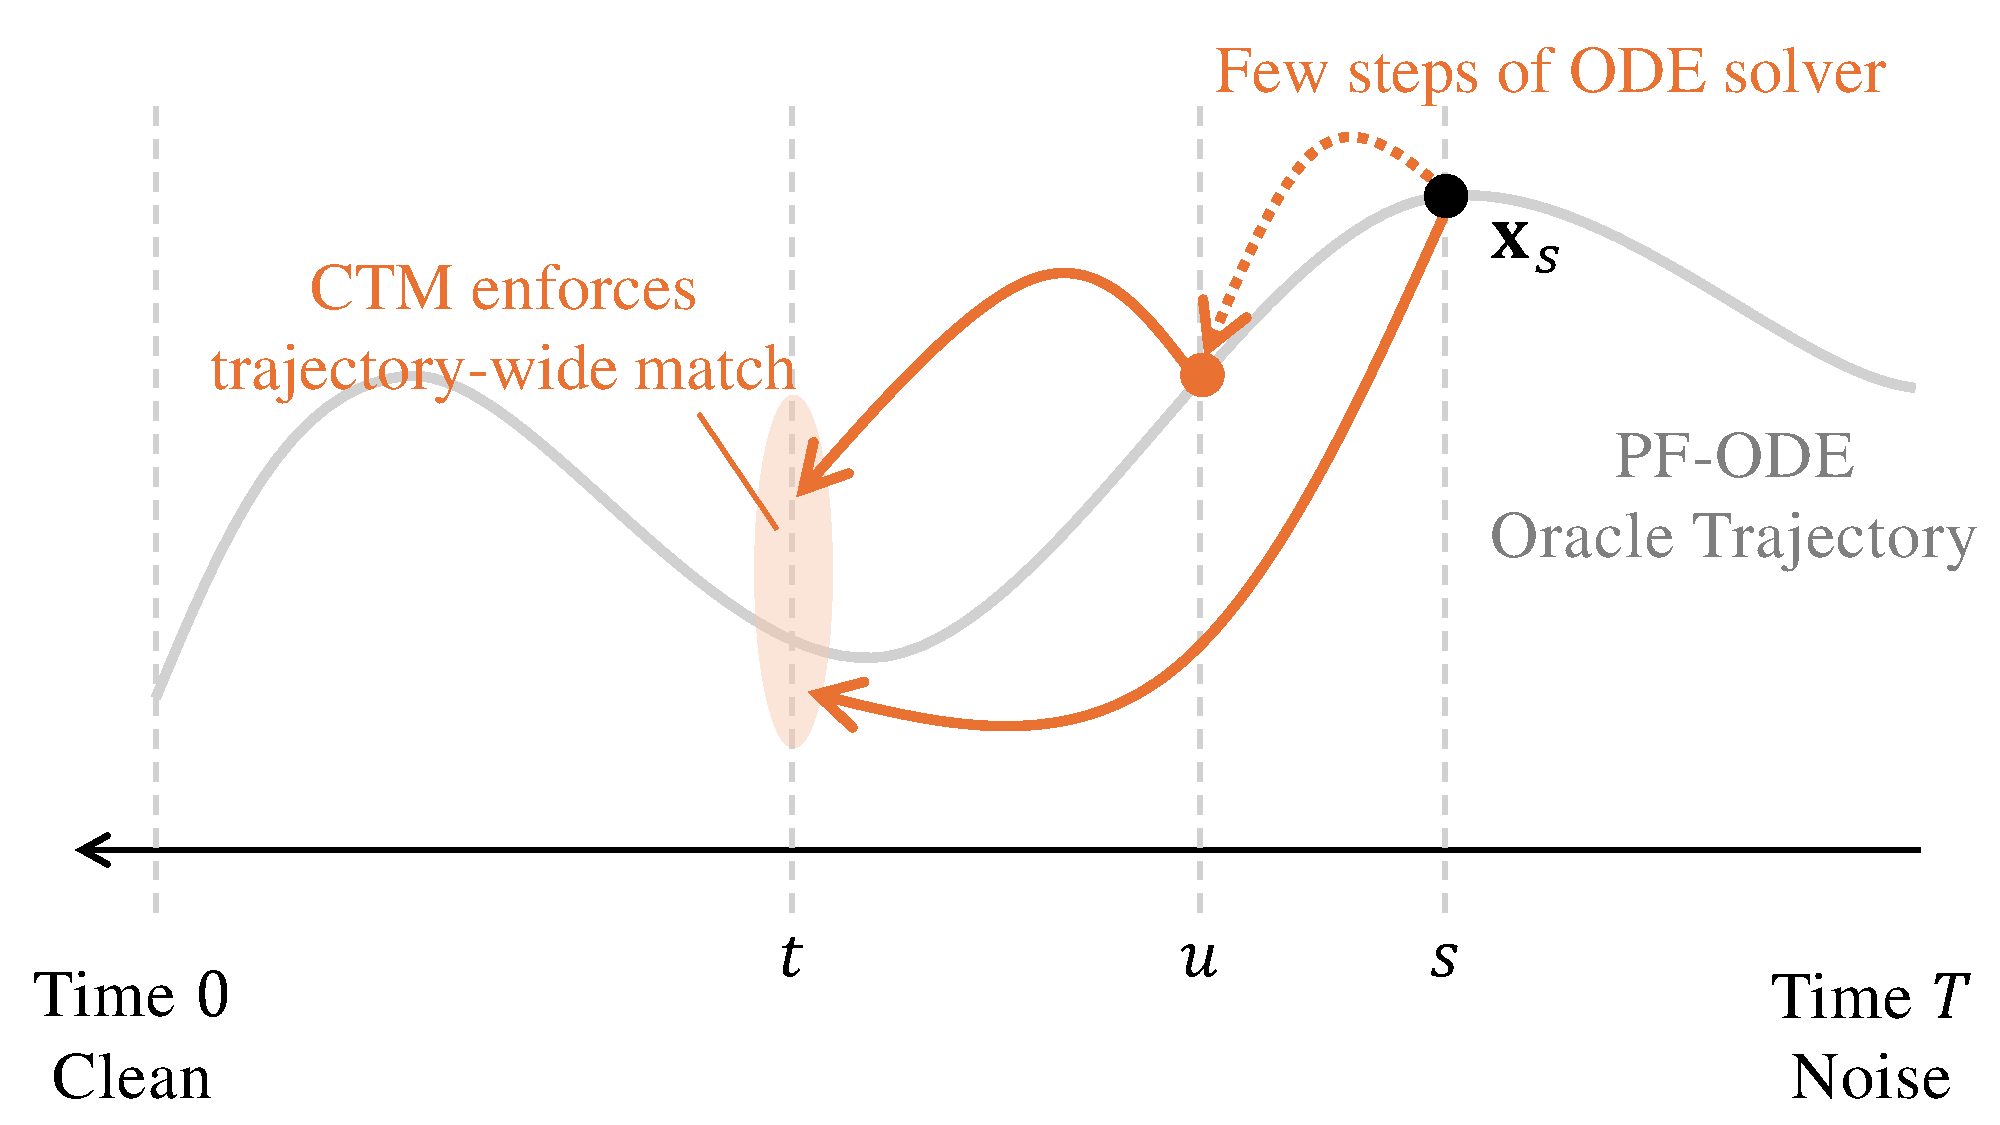
\includegraphics[width=0.9\linewidth]{Images/PartD/ctm-target.pdf}
    \caption{\textbfs{Illustration of CTM's semigroup property.} For any $s \ge u \ge t$, CTM enforces
    $\rmG_{\btheta}(\rvx_s, s,  t)
\approx
\rmG_{\btheta^-} \big(\mathtt{Solver}_{s\to u}(\rvx_s), u ,  t\big)$,
i.e., a short solver segment $s \to u$ followed by a CTM ``jump'' to $t$ matches the direct CTM map $s\to t$. The solver may be a pre-trained diffusion or a CTM's self-induced teacher. \figcredit{Adapted from \citet{kim2023consistency}.}}
    \label{fig:ill_models}
\end{figure}

\subsection{Auxiliary Losses in CTM}\label{subsec:ctm-auxiliary}

(Self-)distillation can underperform the teacher because it optimizes only teacher generated targets, lacking direct supervision from real data. By contrast, CTM can naturally incorporate data driven regularizers, for example by augmenting its objective with denoising score matching and an adversarial (GAN) term~\citep{goodfellow2014generative}, to better learn the flow map. 

\paragraph{Natural Integration of Diffusion Loss.}
The diffusion–model loss (more precisely, the conditional flow matching loss; see \Cref{eq:fm-cfm}) integrates naturally into CTM and provides a fixed regression target that facilitates the learning of the flow map model. To see this, note that we have
\[
\rvv^*(\rvx_s, s)
= \frac{\rvx_s - \rvg^*(\rvx_s, s, s)}{s},
\qquad 
\rvg^*(\rvx_s, s, s) \approx \rvg_{\btheta}(\rvx_s, s, s).
\]
This naturally induces a velocity parametrization through $\rvg_{\btheta}$:
\[
\rvv_{\btheta}(\rvx_s, s)
:= \frac{1}{s}\bigl(\rvx_s - \rvg_{\btheta}(\rvx_s, s, s)\bigr).
\]
Using the linear Gaussian path
\[
\rvx_s = \alpha_s \rvx_0 + \sigma_s \beps,
\qquad
\rvx_0 \sim p_{\mathrm{data}}, 
\beps \sim \mathcal N(0, \mathbf I),
\]
the diffusion model loss can be written as
\begin{align}\label{eq:ctm-dsm}
\mathcal L_{\mathrm{DM}}(\btheta)
&:= 
\E_{\rvx_0, \beps, s}
\Bigl[
w(s)
\bigl\|
 \rvv_{\btheta}(\rvx_s, s) - \left(\alpha_s' \rvx_0 + \sigma_s' \beps\right)
\bigr\|_2^2
\Bigr].
\end{align}



$\mathcal L_{\mathrm{DM}}$ improves accuracy when $t$ is close to $s$ by explicitly supervising small
jumps along the trajectory. In this regime, the factor $1-\tfrac{t}{s}$ in
\Cref{eq:ctm_para_1} approaches zero, which can weaken gradients and slow
learning; $\mathcal L_{\mathrm{DM}}$ supplies a stronger local signal and stabilizes training.  

Conceptually, \Cref{eq:ctm-consist-distill,eq:ctm-consist-scratch} enforce
trajectory matching (zeroth order), while \Cref{eq:ctm-dsm} enforces slope
matching (first order).

\paragraph{(Optional) GAN Loss.}
While consistency and diffusion model loss provide strong regression signals, they can yield
overly smooth outputs. CTM therefore optionally adds an adversarial term to
encourage sharper, more realistic samples by aligning the generator
distribution with the data distribution. With a discriminator
$D_{\bm{\zeta}}$ that distinguishes real $\rvx_{0}\sim p_{\mathrm{data}}$ from
generated $\rvx_{\mathrm{est}}(\rvx_{s},s,t)$, the objective is
\begin{align*} 
&\mathcal{L}_{\mathrm{GAN}}(\bm{\theta}, \bm{\zeta}) := \\ &\mathbb{E}_{\mathbf{x}_0} \big[\log D_{\bm{\zeta}}(\mathbf{x}_0)\big] + \mathbb{E}_{s \in [0, T]} \mathbb{E}_{t \in [0, s]} \mathbb{E}_{\mathbf{x}_0} \mathbb{E}_{\mathbf{x}_s \vert \mathbf{x}_0} \big[\log (1 - D_{\bm{\zeta}}( \mathbf{x}_{\mathrm{est}}(\mathbf{x}_s, s, t)))\big], \end{align*}
where $D_{\bm{\zeta}}$ is maximized and $\rmG_{\bm{\theta}}$ is minimized.
Intuitively, the discriminator acts as an adaptive perceptual distance that
encourages realistic detail. Theoretically, the GAN term drives distributional
matching (Jensen–Shannon divergence) between $p_{\mathrm{data}}$ and the model
distribution induced by $\rmG_{\bm{\theta}}$~\citep{goodfellow2014generative},
which can raise fidelity beyond the teacher.

\paragraph{Overall CTM Objective.}
In summary, CTM unifies (self-)distillation, diffusion, and GAN losses into a single training framework:
\begin{mdframed}
    \begin{align*}
\mathcal{L}_{\mathrm{CTM}}(\bm{\theta},\bm{\zeta})
:=  \mathcal{L}_{\mathrm{consist}}(\bm{\theta};  \bm{\phi}^\times/\bm{\theta}^-)
+ \lambda_{\mathrm{DM}} \mathcal{L}_{\mathrm{DM}}(\bm{\theta})
+ \lambda_{\mathrm{GAN}} \mathcal{L}_{\mathrm{GAN}}(\bm{\theta},\bm{\zeta}),
\end{align*}
\end{mdframed}
where the teacher is either an external pre-trained model $\bm{\phi}^\times$ or
the self-induced teacher $\bm{\theta}^-$. The regression style components
$\mathcal{L}_{\mathrm{consist}}$ and $\mathcal{L}_{\mathrm{DM}}$ act as strong
regularizers, while the optional GAN term improves fine scale detail without
sacrificing stability~\citep{kim2024pagoda}.


\subsection{Flexible Sampling with CTM}
CTM learns the general flow map $\bPsi_{s\to t}$ for any $s>t$, which means it supports
anytime to anytime transitions. This property enables flexible sampling strategies. 
For example, CTM proposes \emph{$\gamma$ sampling}, where the hyperparameter $\gamma$
controls the stochasticity during generation.
In addition, CTM can reuse standard inference techniques developed for diffusion models,
such as ODE based solvers and exact likelihood computation.

In what follows, we fix a discrete time grid for sampling $T=\tau_0 > \tau_1 > \tau_2 > \cdots > \tau_{M}=0$.

\begin{algorithm}[H]
    \centering
    \caption{CTM's $\gamma$-sampling}\label{alg:gamma}
    \begin{algorithmic}[1]
    \Require Trained CTM $\mathbf{G}_{\bm{\theta}^\times}$, $\gamma\in[0,1]$, $T=\tau_0>\tau_1 > \tau_2 > \cdots > \tau_{M}=0$.
    \State Start from $\mathbf{x}_{\tau_{0}}\sim p_{\mathrm{prior}}=\mathcal{N}(\bm{0}, T^2\rmI)$
        \For{$n=0$ to $M-1$}
        \State $\tilde{\tau}_{n+1}\leftarrow \sqrt{1-\gamma^{2}}\tau_{n+1}$
        \State Denoise $\mathbf{x}_{\tilde{\tau}_{n+1}}\leftarrow \mathbf{G}_{\bm{\theta}^\times}(\mathbf{x}_{\tau_{n}},\tau_{n},\tilde{\tau}_{n+1})$
        \State Diffuse $\mathbf{x}_{\tau_{n+1}}\leftarrow\mathbf{x}_{\tilde{\tau}_{n+1}}+\gamma \tau_{n+1}\bm{\epsilon}$, where $\bm{\epsilon}\sim\mathcal{N}(\bm{0}, \rmI)$
        \EndFor
        \Ensure  $\mathbf{x}_{\tau_{M}}$
    \end{algorithmic}
\end{algorithm}

\paragraph{Methodology of $\gamma$-Sampling.}
CTM's $\gamma$-sampling introduces a unified family of samplers that arises naturally from learning a general flow map model.  
It encompasses prior approaches, such as CM's multistep sampling (see \Cref{alg:cm_sampling}) 
and time-stepping-style sampling, which is conceptually similar to ODE solvers.  
The parameter $\gamma$ directly controls the degree of semantic change during generation, 
making $\gamma$ sampling a flexible and task aware strategy for diverse downstream applications.





\begin{figure}[t]
    \centering
    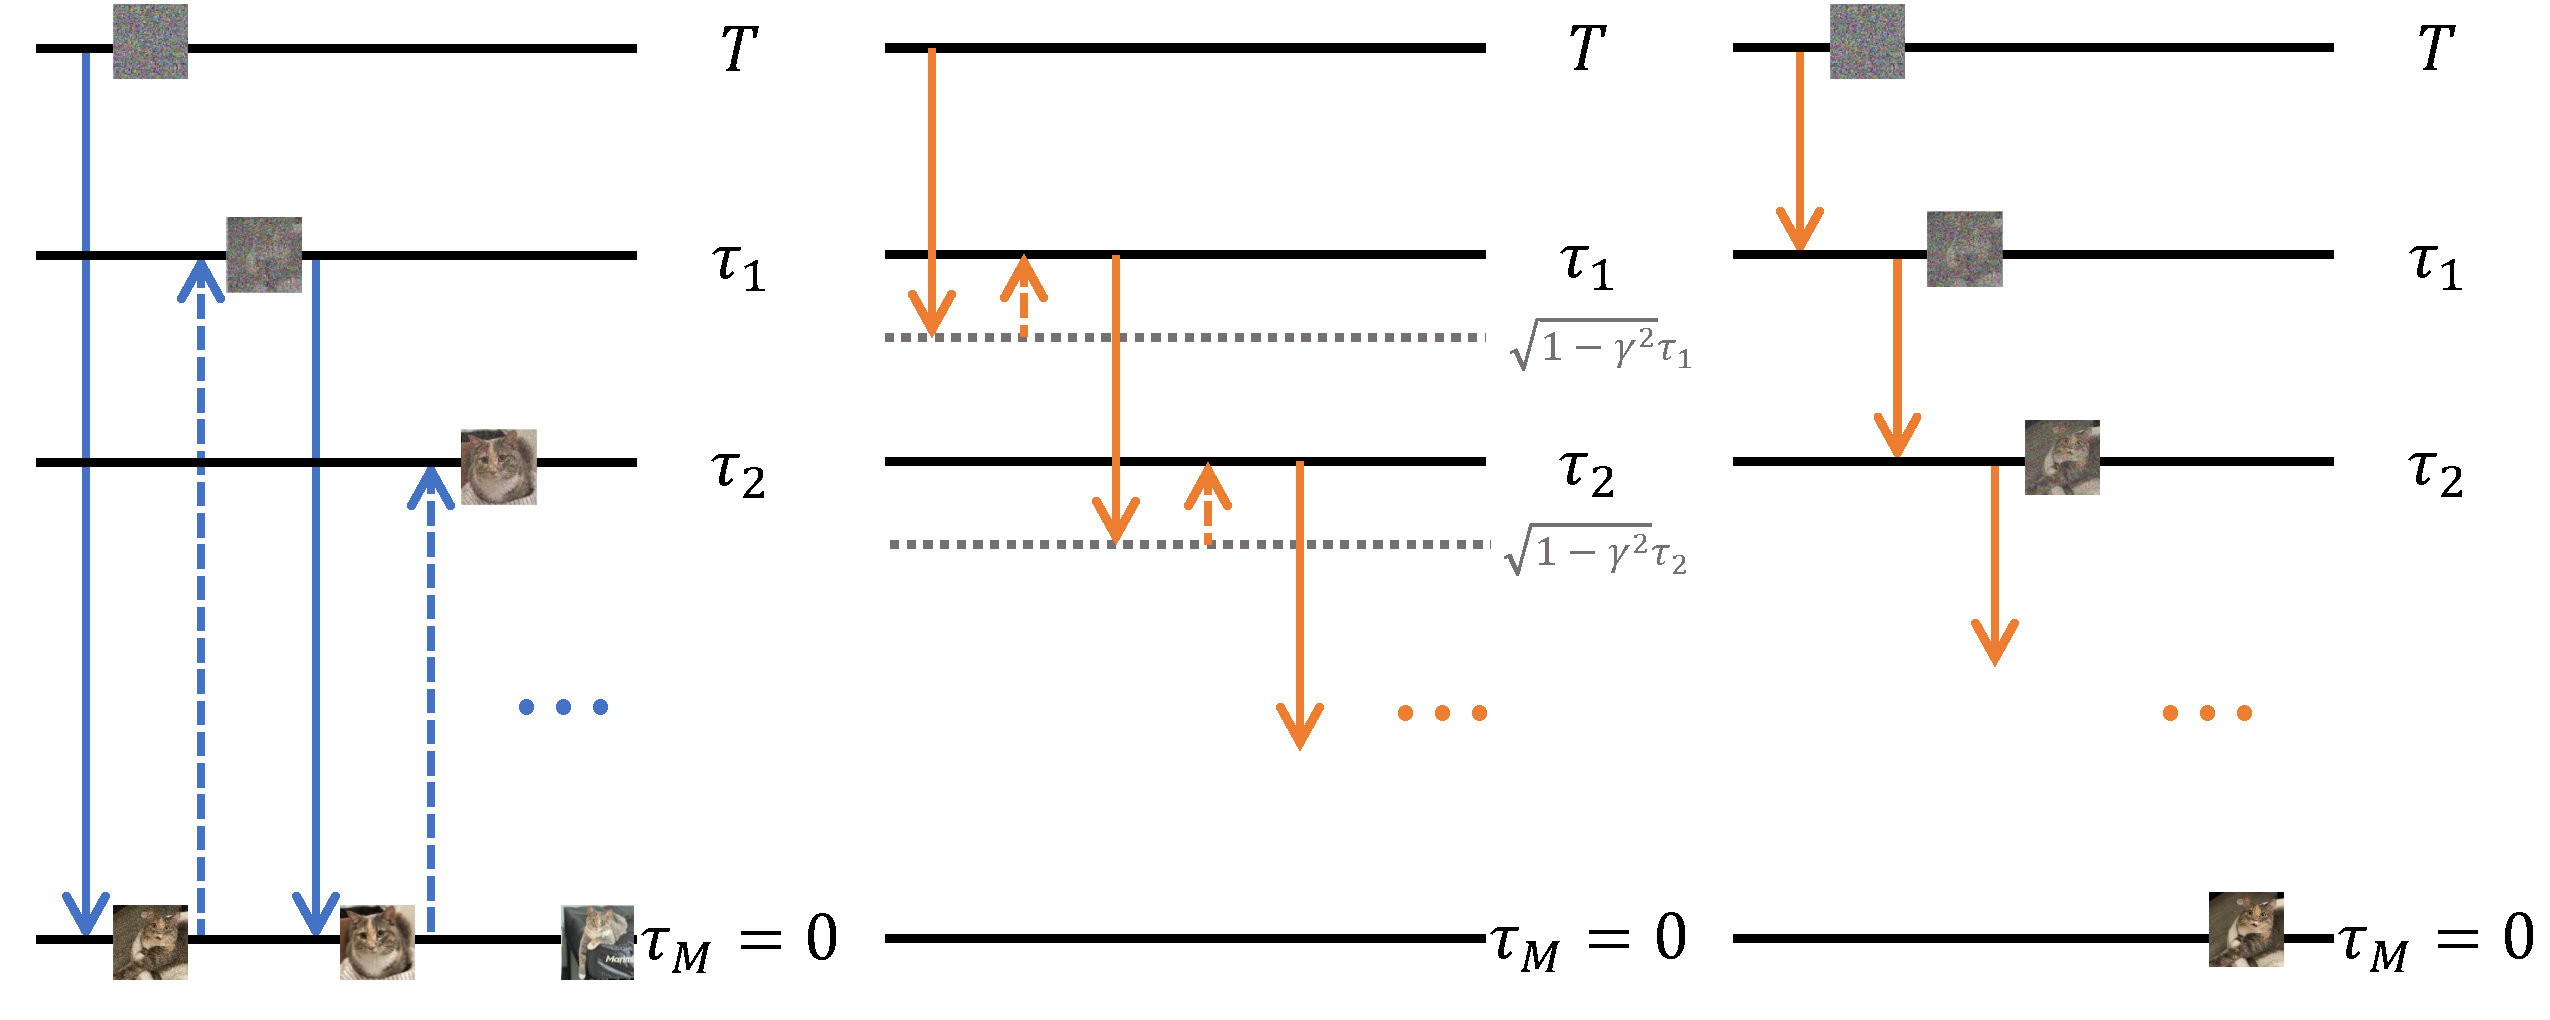
\includegraphics[width=\linewidth]{Images/PartD/ctm_gamma.pdf}
    \caption{\textbfs{Illustration of $\gamma$-sampling with varying $\gamma$ value.} The procedure alternates between denoising with a network evaluation and adding noise in reverse,   $(\tau_{n}\xrightarrow{\text{Denoise}} \sqrt{1-\gamma^{2}}\tau_{n+1}\xrightarrow{\text{Noisify}} \tau_{n+1})_{n=0}^{M-1}$.
The leftmost panel illustrates $\gamma=1$, corresponding to the fully stochastic case.  
The rightmost panel shows $\gamma=0$, corresponding to the fully deterministic case.  
The middle panel depicts intermediate values $\gamma\in(0,1)$, which interpolate between these two extremes. 
\figcredit{Adapted from \citet{kim2023consistency}.}}
    \label{fig:gamma_sampling}
\end{figure}


\begin{itemize}
\item \Cref{fig:gamma_sampling}-(Left): When $\gamma=1$, it coincides with the multistep sampling introduced in CM (i.e., a special flow map $\bPsi_{s\to 0}$), which is fully stochastic and results in semantic variation when the number of steps changes.

\item \Cref{fig:gamma_sampling}-(Right): When $\gamma=0$, it reduces to fully deterministic time-stepping, which estimates the solution trajectory of the PF-ODE. A key distinction between $\gamma$ sampling with $\gamma=0$ and conventional time-stepping ODE-based sampling is that CTM avoids the discretization errors of numerical solvers.

\item \Cref{fig:gamma_sampling}-(Middle): When $0 < \gamma < 1$, $\gamma$-sampling interpolates between the two extremes by allowing a controlled amount of stochasticity to be injected during sampling. 
\end{itemize}
We highlight that values $\gamma\in[0,1)$ require the general flow map
$\bPsi_{s\to t}$, whereas the special case $\gamma=1$ reduces to
CM-style multistep sampling and requires only $\bPsi_{s\to0}$.

\paragraph{Analysis of $\gamma$-Sampling.} CTM empirically observed that CM's multistep sampling degrades in quality once the number of steps $M \geq 4$.  
To explain this phenomenon, CTM analyzed the underlying cause: when $\gamma \neq 0$, each neural ``jump'' introduces a small mismatch, and these mismatches accumulate as the model iteratively maps states toward time zero. This error accumulation explains why long multi-step runs can perform poorly. We formalize this idea in the following proposition.

\proppp{(Informal) 2-step $\gamma$-sampling}{ctm-gamma}{
\label{th:sampling_agg_error_2_steps}
Let $\tau\in(0,T)$ and $\gamma \in [0,1]$. Let $p_{\bm{\theta}^{*},2}$ denote as the density obtained from the $\gamma$-sampler with the optimal CTM, following the transition sequence $
    T\rightarrow\sqrt{1-\gamma^2}\tau\rightarrow \tau \rightarrow 0
$, starting from $p_T$. Then
 \begin{align*}
    \mathcal D_{\mathrm{TV}}\big( p_{\mathrm{data}}, p_{\bm{\theta}^{*},2} \big)         = \mathcal{O}\left(\sqrt{T-\sqrt{1-\gamma^2}\tau+ \tau}  \right).
 \end{align*}
 Here, $\mathcal{D}_{\mathrm{TV}}$ denotes the total variation  between distributions (see \Cref{eq:f-div}).
}{
We refer the reader to Theorem 8 of~\citet{kim2023consistency} for the general case when the number of sampling steps is $M$. }
The insights from the above theorem can be summarized as follows:
\begin{itemize}
    \item \textbfs{When} $\gamma = 1$ (corresponding to CM's multistep sampling)\textbfs{:} The method performs iterative long-range transitions from $\tau_n$ to $0$ at each step $n$. This leads to error accumulation on the order of
    \begin{align*}
        \mathcal{O}\left(\sqrt{T + \tau_1 + \cdots + \tau_M}\right).
    \end{align*}
    
    \item \textbfs{When} $\gamma = 0$ (corresponding to CTM's deterministic multistep sampling)\textbfs{:} Such temporal overlap between transitions is eliminated. This avoids error accumulation and yields a tighter bound of $\mathcal{O}(\sqrt{T})$. Empirically, CTM with $\gamma = 0$ provides a favorable trade-off between sampling speed and sample quality: increasing the number of sampling steps improves generation quality without introducing instability.
\end{itemize}


\paragraph{CTM Supports Diffusion Inference.} Since CTM learns the score function (or denoiser) directly through $\rvg_{\bm{\theta}}$, 
thanks to its parametrization in \Cref{eq:ctm_para_1}, it is compatible with inference techniques 
originally developed for diffusion models. For instance, one can compute exact likelihoods 
(\Cref{subsec:sde-sample}) or apply advanced samplers such as DDIM or DPM (\Cref{ch:solvers}) 
for generation, by using $\rvg_{\bm{\theta}}(\cdot, s, s)$.




\newpage

\section{\texorpdfstring{General Flow Map: Mean Flow}{General Flow Map: Mean Flow}}\label{sec:MF}


Just as diffusion models admit many equivalent parameterizations and training objectives, a general flow map $\bPsi_{s\to t}$ can also be learned in multiple plausible ways.  
In this section, we introduce \emph{Mean Flow} (MF)~\citep{geng2025mean}, a later representative of the general flow map family $\bPsi_{s\to t}$ that illustrates an alternative yet principled perspective on how such maps can be effectively learned.



\subsection{Modeling and Training of Mean Flow}

In contrast to CM and CTM, which build on the EDM framework, MF is based on the 
flow matching formulation ($\alpha_t = 1-t$ and $\sigma_t  = t$ for $t\in[0,1]$). 
Rather than directly parameterizing the flow map, MF learns the \emph{average drift}
over an interval $[t,s]$ (with $t<s$):
\[
\rvh_{\btheta}(\rvx_s, s, t)  \approx 
\rvh^*(\rvx_s, s, t) := \frac{1}{t-s}\int_s^t \rvv^*(\rvx_u,u) \diff u.
\]
The corresponding oracle loss is
\begin{align}\label{eq:mf-oracle}
\mathbb{E}_{t<s} \mathbb{E}_{\rvx_s\sim p_s}\Big[w(s) 
\|\rvh_{\btheta}(\rvx_s,s,t) - \rvh^*(\rvx_s,s,t)\|_2^2\Big].
\end{align}
In particular, when $s \to t$, the loss function reduces to the flow matching loss:
\begin{align}\label{eq:mf-to-fm}
    \mathbb{E}_{t} \mathbb{E}_{\rvx_t\sim p_t}\Big[w(t) 
\|\rvh_{\btheta}(\rvx_t,t,t) - \rvv^*(\rvx_t,t)\|_2^2\Big],
\end{align}
learning the instantaneous velocity.
We will see later in \Cref{subsec:equivalence-ctm-mf} that MF remains consistent with the 
general objective in \Cref{eq:general-cm-loss:rep}, 
but approaches it from a different (while equivalent) perspective.
Since the oracle regression target $\rvh^*(\rvx_s,s,t)$ does not admit a closed form in general, MF constructs a surrogate by exploiting an identity obtained from differentiating
\[
(t-s)\,\rvh^*(\rvx_s,s,t) = \int_s^t \rvv^*(\rvx_u,u)\,\diff u
\]
with respect to $s$. This yields the \emph{MF identity}:
\begin{align}\label{eq:mf-identity}
\begin{aligned}
    \rvh^*(\rvx_s,s,t)
&= \rvv^*(\rvx_s,s) - (s-t) \tfrac{\diff}{\diff s}\rvh^*(\rvx_s,s,t) \\
&= \rvv^*(\rvx_s,s) - (s-t)\Big[(\partial_{\rvx}\rvh^*)(\rvx_s,s,t) \rvv^*(\rvx_s,s) 
+ \partial_s \rvh^*(\rvx_s,s,t)\Big],
\end{aligned}
\end{align}
where the second line applies the chain rule together with 
\[
\frac{\diff}{\diff s}\rvx_s = \rvv^*(\rvx_s,s).
\]

Motivated by this identity, MF replaces the intractable oracle with a stop-gradient surrogate, leading to the practical training objective
\begin{mdframed}
\begin{align}\label{eq:mf-practice}
    \mathcal{L}_{\mathrm{MF}}(\btheta)
:= \mathbb{E}_{t<s} \mathbb{E}_{\rvx_s\sim p_s}\Big[w(s)\,
\|\rvh_{\btheta}(\rvx_s,s,t) - \rvh_{\btheta^-}^{\mathrm{tgt}}(\rvx_s,s,t)\|_2^2\Big],
\end{align}
\end{mdframed}
where the regression target is defined as
\begin{align*}
    \rvh_{\btheta^-}^{\mathrm{tgt}}&(\rvx_s,s,t)
:= \\ &\rvv^*(\rvx_s,s) - (s-t)\Big[\underbrace{(\partial_{\rvx}\rvh_{\btheta^-})(\rvx_s,s,t) \rvv^*(\rvx_s,s)
+ \partial_s \rvh_{\btheta^-}(\rvx_s,s,t)}_{\mathrm{JVP}}\Big].
\end{align*}

In practice, the oracle velocity $\rvv^*$ cannot be computed in closed form and
must instead be approximated. Two common strategies are available: relying on a
pre-trained diffusion model (\emph{distillation}) or constructing a direct
estimator from data (\emph{training from scratch}). Regardless of the choice, one ultimately needs to compute a
\emph{Jacobian--vector product}  (JVP) of the target network
$\rvh_{\btheta^-}$:
\[ 
\left[\partial_\rvx \rvh_{\btheta^-}, \partial_s \rvh_{\btheta^-}, \partial_t \rvh_{\btheta^-}\right]^\top \cdot \left[\rvv^*, 1, 0\right]
\]


\paragraph{Distillation.}
Use a pre-trained diffusion model with a flow matching backbone,
$\rvv_{\bphi^\times} \approx \rvv^*$.

\paragraph{Training from scratch.}
Use the one point conditional velocity $\alpha_s'\rvx_0 + \sigma_s'\beps$,
obtained from the forward noise injection $\rvx_s=\alpha_s\rvx_0+\sigma_s\beps$ with
$\beps\sim\mathcal N(\bm{0},\rmI)$. This gives an unbiased single sample estimate of the
instantaneous drift at level $s$ when evaluated at paired $(\rvx_0,\beps)$.

% We emphasize that MF’s strength lies in its strong performance in the training-from-scratch setting. It requires no pre-trained model for initialization or guidance during training, and it does not rely on additional regularizers (such as a GAN loss). In this sense, MF serves as a fully standalone generative model.

\subsection{Sampling of Mean Flow}
Once a MF $\rvh_{\btheta^\times}$ is trained, it naturally recovers a proxy of the flow
map. For any starting point $\rvx_s$, the map from $s$ to $t$ is (approximately) given by
\[
\bPsi_{s\to t}(\rvx_s) = \rvx_s + (t-s)\,\rvh^*(\rvx_s,s,t)
  \approx   \rvx_s + (t-s)\,\rvh_{\btheta^\times}(\rvx_s,s,t).
\]

This enables both one-step and multi-step sampling. For example, drawing
$\rvx_T\sim p_{\mathrm{prior}}$, the one-step generation of a clean sample is
\[
\rvx_0  \leftarrow  \rvx_T - T\,\rvh_{\btheta^\times}(\rvx_T,T,0).
\]

Alternatively, multi-step generation can be performed by preparing a time grid
and applying the map sequentially, in the same time-stepping manner used in
CTM. Since MF learns a general flow map, it also supports $\gamma$-sampling
as in CTM, where a controllable hyperparameter $\gamma$ injects stochasticity
into the sampling process.



\subsection{Relationship between CTM and MF}\label{subsec:equivalence-ctm-mf}
At first sight CTM and MF may appear unrelated.  
In fact, both provide different parameterizations of the same oracle flow
map $\bPsi_{s\to t}$, and their corresponding squared oracle regression
errors are related by a time-dependent weighting~\citep{hu2025cmt}.

\paragraph{Relationship of Parameterizations.}
Both methods operate under the same general framework but represent the learned function in distinct ways.  
The flow map can be written equivalently as
\begin{align*}
\bPsi_{s\to t}(\rvx_s)
& = \rvx_s + \int_s^t \rvv^*(\rvx_u, u)\diff u \\
&= \frac{t}{s}\rvx_s
   + \frac{s-t}{s}\underbrace{\Bigg[\rvx_s + \frac{s}{s-t}\int_s^t \rvv^*(\rvx_u,u)\,\diff u\Bigg]}_{\approx\,\rvg_\btheta} \\
&= \rvx_s + (t-s)\underbrace{\Bigg[\frac{1}{t-s}\int_s^t \rvv^*(\rvx_u,u)\,\diff u\Bigg]}_{\approx\,\rvh_\btheta}.
\end{align*}
Here, the first is the definition of the flow map, the second form highlights the CTM parametrization through $\rvg_\btheta$ (see \Cref{eq:ctm-g-oracle,eq:ctm_para_1}), while the last highlights the MF parametrization through $\rvh_\btheta$.  


\paragraph{Relationship of Training Loss.} Given the above reinterpretation of the oracle flow map $\bPsi_{s\to t}$ in terms of the CTM parametrization 
\[
\rvg_\btheta(\rvx_s,s,t) \approx \rvg^*(\rvx_s,s,t):=\rvx_s + \frac{s}{s-t}\int_s^t \rvv^*(\rvx_u,u) \diff u
\]
 and the MF parametrization 
\[
\rvh_\btheta(\rvx_s,s,t) \approx \rvh^*(\rvx_s,s,t):=\frac{1}{t-s}\int_s^t \rvv^*(\rvx_u,u) \diff u,
\] 
we now show that the training losses of CTM and MF are in fact equivalent.


Consider the relation
\[
\rvg_\btheta(\rvx_s,s,t) := \rvx_s - s \rvh_\btheta(\rvx_s,s,t),
\]
and take $d(\rvx,\rvy):=\|\rvx-\rvy\|^2$ as an example. Substituting into \Cref{eq:general-cm-loss:rep} and viewing $\rmG_\btheta$ as CTM’s flow-map parameterization (\Cref{eq:ctm_para_1}) gives
\begin{align} &~d\big(\rmG_\btheta(\rvx_s,s,t), \bPsi_{s\to t}(\rvx_s)\big) \notag \\ = &~\norm{\rmG_\btheta(\rvx_s,s,t) - \bPsi_{s\to t}(\rvx_s)}^2 \notag \\ = &~\norm{\left(\frac{t}{s}\rvx_s + \frac{s-t}{s} \rvg_\btheta(\rvx_s,s,t)\right)-\left(\frac{t}{s}\rvx_s + \frac{s-t}{s}\Big[\rvx_s + \frac{s}{s-t}\int_s^t \rvv^*(\rvx_u,u) \diff u\Big]\right)}^2 \notag \\ = &~\left(\frac{s-t}{s}\right)^2\norm{\rvg_\btheta(\rvx_s,s,t)-\left(\rvx_s + \frac{s}{s-t}\int_s^t \rvv^*(\rvx_u,u) \diff u\right)}^2 \label{eq:g-para} \\ = &~\left(\frac{s-t}{s}\right)^2\norm{\left(\rvx_s - s \rvh_\btheta(\rvx_s,s,t)\right)-\left(\rvx_s + \frac{s}{s-t}\int_s^t \rvv^*(\rvx_u,u) \diff u\right)}^2 \notag \\ = &~\left(\frac{s-t}{s}\right)^2\norm{\left(\rvx_s - s \rvh_\btheta(\rvx_s,s,t)\right)-\left(\rvx_s + \frac{s}{s-t}\int_s^t \rvv^*(\rvx_u,u) \diff u\right)}^2 \notag \\ = &~\left(s-t\right)^2\norm{ \rvh_\btheta(\rvx_s,s,t)- \left(\frac{1}{t-s}\int_s^t \rvv^*(\rvx_u,u)\diff u \right)}^2 \label{eq:h-para} \end{align}
Hence,
\begin{align*} 
\frac{1}{s^2} \Bigg\|\rvg_\btheta(\rvx_s,s,t)-\rvg^*(\rvx_s,s,t) \Bigg\|^2 = \Bigg\|\rvh_\btheta(\rvx_s,s,t)-\rvh^*(\rvx_s,s,t) \Bigg\|^2. 
\end{align*}
Putting aside the specific algorithm used to learn the flow map, the CTM and MF losses share the same mathematical form, differing only by a weighting function. Moreover, setting $t=0$ in either case recovers the CM setting ($\bPsi_{s\to 0}$), where
each state maps directly to the clean data.

\paragraph{Auxiliary Loss in Practice.}
In CTM, training is performed with the consistency loss in \Cref{eq:ctm-consist-scratch} jointly with its self-defined diffusion model loss in \Cref{eq:ctm-dsm}. A similar strategy is adopted in MF. As shown in \Cref{eq:mf-to-fm}, when $s \to t$, the MF loss reduces to the standard flow matching objective. In practice, MF controls the ratio between pairs with $s \neq t$ and those with $s = t$; consequently, the overall optimization becomes a mixture of the MF objective in \Cref{eq:mf-practice} and the flow matching objective in \Cref{eq:mf-to-fm}. 

Both parametrizations are able to provide a smooth transition from diffusion-model training, which learns instantaneous velocity with a fixed regression target, to flow-map learning, which employs a stop-gradient pseudo-regression target.


\paragraph{Both CTM and MF Parameterizations Enable Flexible Inference.}
Both CTM ($\rmG_\btheta(\rvx_s,s,t)$) and MF ($\rvh_\btheta(\rvx_s,s,t)$) aim to approximate the underlying flow map $\bPsi_{s\to t}$:
\[
\rmG_\btheta(\rvx_s,s,t)\approx\bPsi_{s\to t},\quad  \text{and}
\quad 
\rvx_s+(t-s)\rvh_\btheta(\rvx_s,s,t)\approx\bPsi_{s\to t}.
\]
Since both models learn an explicit mapping between any two time steps, they naturally support CTM’s $\gamma$-sampling and remain compatible with inference techniques originally developed for diffusion models, such as guidance (\Cref{ch:guidance}), exact likelihood computation (\Cref{eq:score-sde-likelihood}), and accelerated sampling with higher-order solvers (\Cref{ch:solvers}). 
This compatibility arises because their parameterizations recover the instantaneous diffusion drift in the infinitesimal limit $t\to s$:
\[
\rvg^*(\rvx_s,s,s)=\rvx_s-s\,\rvv^*(\rvx_s,s),
\quad  \text{and}
\quad 
\rvh^*(\rvx_s,s,s)=\rvv^*(\rvx_s,s).
\]
This property is not shared by specialized flow map formulations $\bPsi_{s\to0}$, such as those in the CM family. Thus, both CTM and MF can be regarded as flexible and general flow map formulations that generalize diffusion-based inference to direct time-to-time mappings.




\paragraph{Conclusion.}
% This equivalence between CTM and MF is similar to the situation in diffusion models (\Cref{sec:equivalent-parametrizations}), where different parameterizations ultimately describe the same underlying oracle target. In principle, these formulations are mathematically identical. In practice, however, their behavior can differ because of factors such as loss weighting, network design, or optimization dynamics, which may cause one approach to perform better than another under specific conditions.


The relationship between CTM and MF is analogous to the relationship between
different parametrizations of diffusion models
(\Cref{sec:equivalent-parametrizations}): at the oracle level, they encode the
same underlying flow map. Under squared-error regression and the parametrization
relation above, their oracle regression errors differ only by a known
time-dependent scaling. Their practical training objectives, however, remain
different because they use different surrogate targets and optimization
procedures.

Although CTM and MF are related in this way, they differ conceptually and algorithmically in how the target is learned. The CTM target is defined in the ``integral'' form, as it acts directly on the flow map. The MF target, on the other hand, is defined in the ``differential'' form, as it relies on finite differences of the flow map. Because a target in the integral form is not directly tractable, CTM must solve an ODE during training. In contrast, MF leverages the MF identity (see \Cref{eq:mf-identity}) to construct a tractable target in the differential form. This relationship is analogous to that between energy-based and score-based methods: the former learns a probability density itself (in the integral form), while the latter matches the gradient of that density (in the differential form). In practice, CTM and MF may behave differently due to factors such as loss weighting, network architecture, and optimization dynamics, which can cause one method to perform better than the other under certain conditions.

This perspective suggests that CTM and MF are not the only viable formulations. Other parameterizations of the flow map could also enable efficient and stable training, potentially leading to new standalone generative models. Exploring these alternatives may further enrich the landscape of diffusion models and their flow map extensions, pushing the boundaries of few-step generation.

\clearpage
\newpage

\section{Closing Remarks}\label{sec:ch11_cr}

This final chapter has brought our exploration full circle: from slow iterative
diffusion samplers to fast few-step generators (learned from scratch). The common object behind the methods in this chapter is the oracle flow map
introduced in \Cref{eq:general-cm-loss:rep}:
\[
\bPsi_{s\to t}(\rvx_s)
=
\rvx_s+\int_s^t \rvv^*(\rvx_\tau,\tau)\,\diff \tau.
\]
Learning this map replaces many small numerical updates by one or a few learned
jumps.


At this point, it is useful to step back from the individual algorithms.
Knowledge Distillation (\Cref{sec:distillation-prologue}), Progressive
Distillation (\Cref{sec:PD}), CM (\Cref{sec:discrete-cm}), CTM
(\Cref{sec:CTM}), and MF (\Cref{sec:MF}) were introduced through
different training constructions, but they all exploit, explicitly or
implicitly, the same ODE solution-map structure.

The flow map itself is a classical object from differential equations and
dynamical systems, with closely related particle-based and field-based
descriptions in continuum and fluid mechanics; see
\Cref{eq:flow-map-def} and the surrounding historical discussion.
Here, we use three classical descriptions of the same ODE flow, namely
the \emph{semigroup}, \emph{Lagrangian}, and \emph{Eulerian} views, as an
organizing lens for the modern learning methods developed above%
\footnote{In modern generative modeling, \citet{boffi2024flow} bring together
structural ideas that already appear across PD, CM, CTM, and MF, and use them to
describe the learning of diffusion PF-ODE flow maps in a common language. The
main ingredients therefore largely come from these existing lines of work. Our
presentation and illustrations in this part are also informed by the exposition
of \citet{dieleman2026flowmaps}.}


\paragraph{Semigroup View: Split the Trip.}
As introduced in \Cref{eq:semi-group}, the finite-step identity is
\[
\bPsi_{u\to t}\big(\bPsi_{s\to u}(\rvx_s)\big)
=
\bPsi_{s\to t}(\rvx_s).
\]
As illustrated in \Cref{fig:semigroup}, the intuition is the same as traveling along a fixed route: going from $s$ to
$u$ and then from $u$ to $t$ lands at the same point as going directly from
$s$ to $t$.  Within this view, KD learns the full transition $\bPsi_{T\to0}$, PD
compresses two adjacent teacher steps into one student step, CM learns the
special anytime-to-clean map $\bPsi_{s\to0}$, and CTM extends the same
composition principle to the general map $\bPsi_{s\to t}$.

\begin{figure}[t]
    \centering

    \begin{subfigure}[t]{0.485\textwidth}
        \centering
        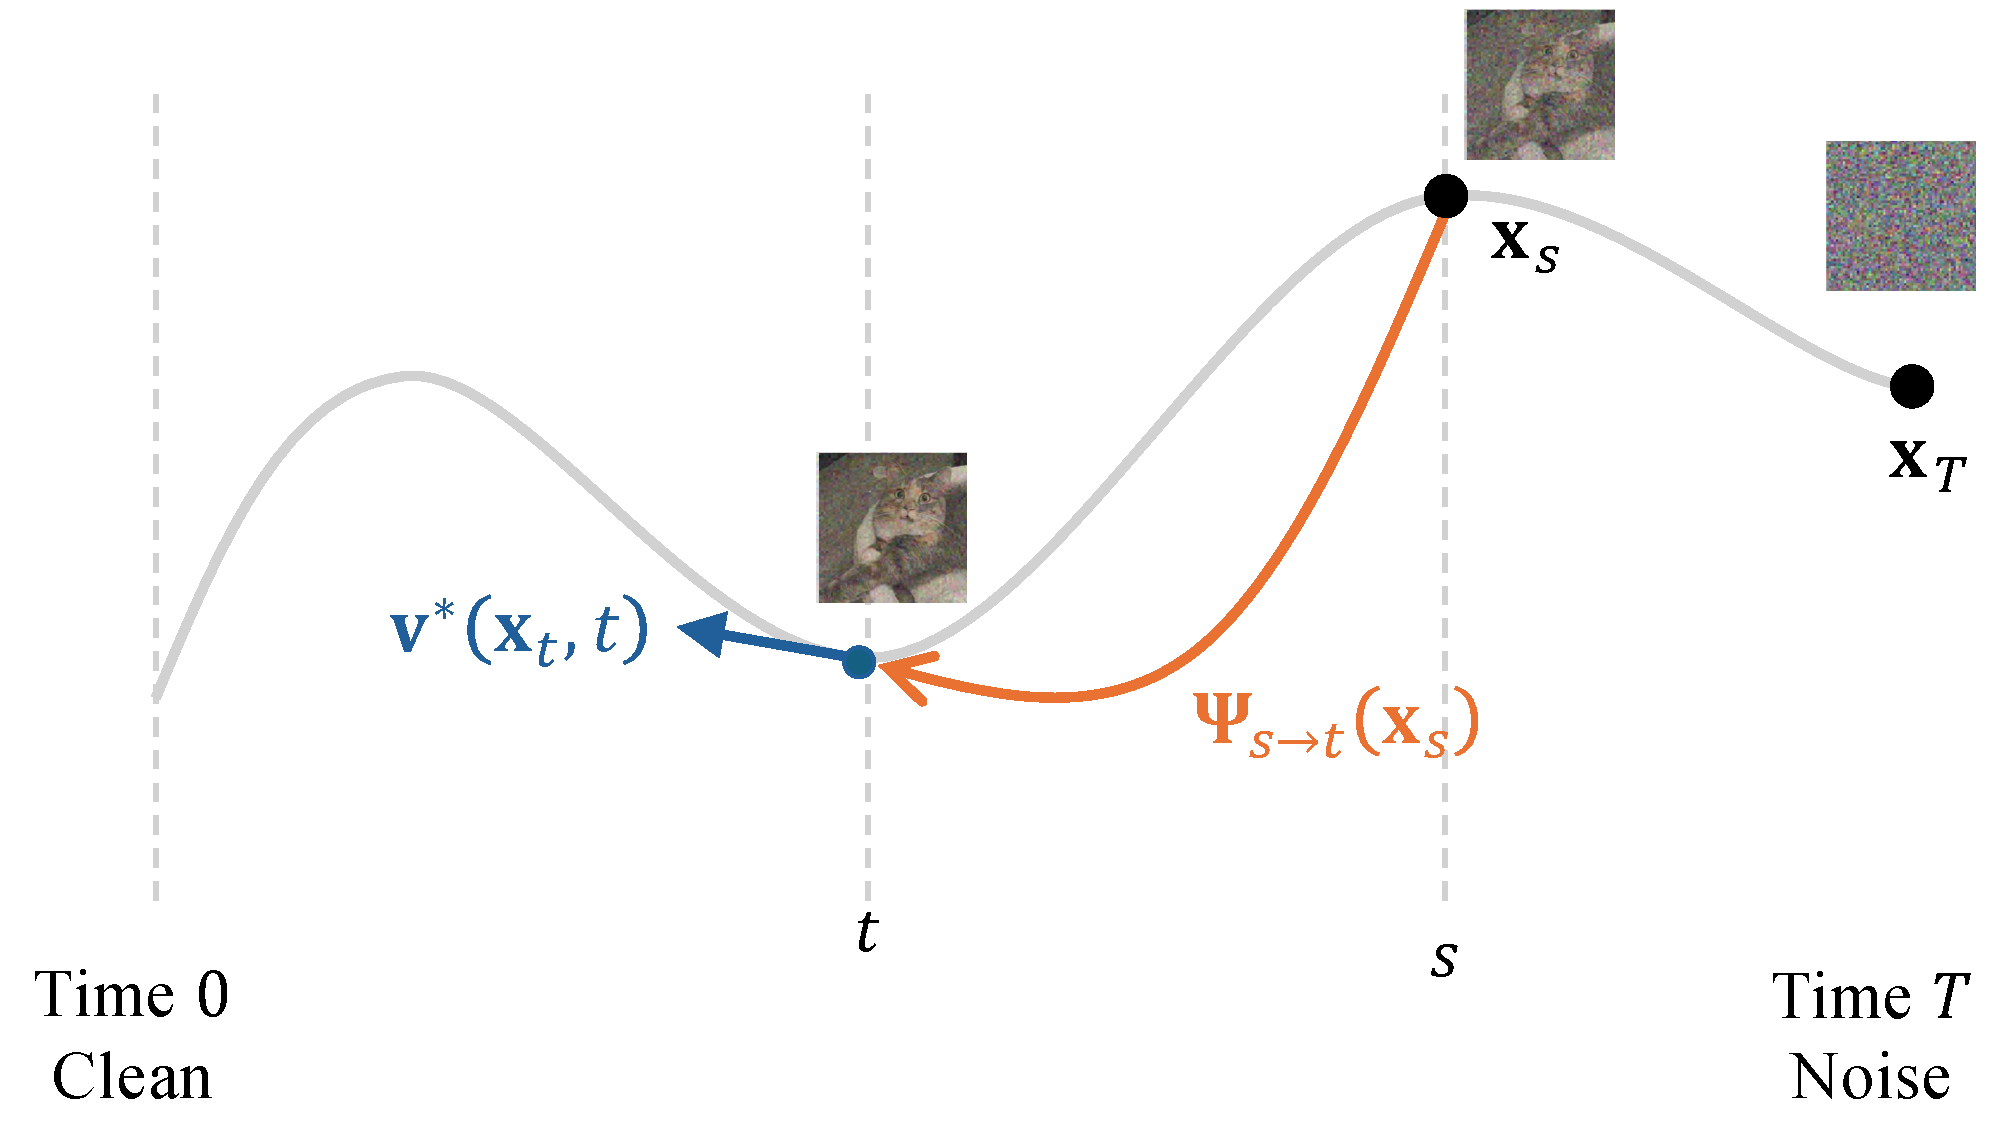
\includegraphics[width=\linewidth]{Images/PartD/lagrangian-1.pdf}
        \caption{Base ending time $t$.}
        \label{fig:lagrangian-base}
    \end{subfigure}
    \hfill
    \begin{subfigure}[t]{0.485\textwidth}
        \centering
        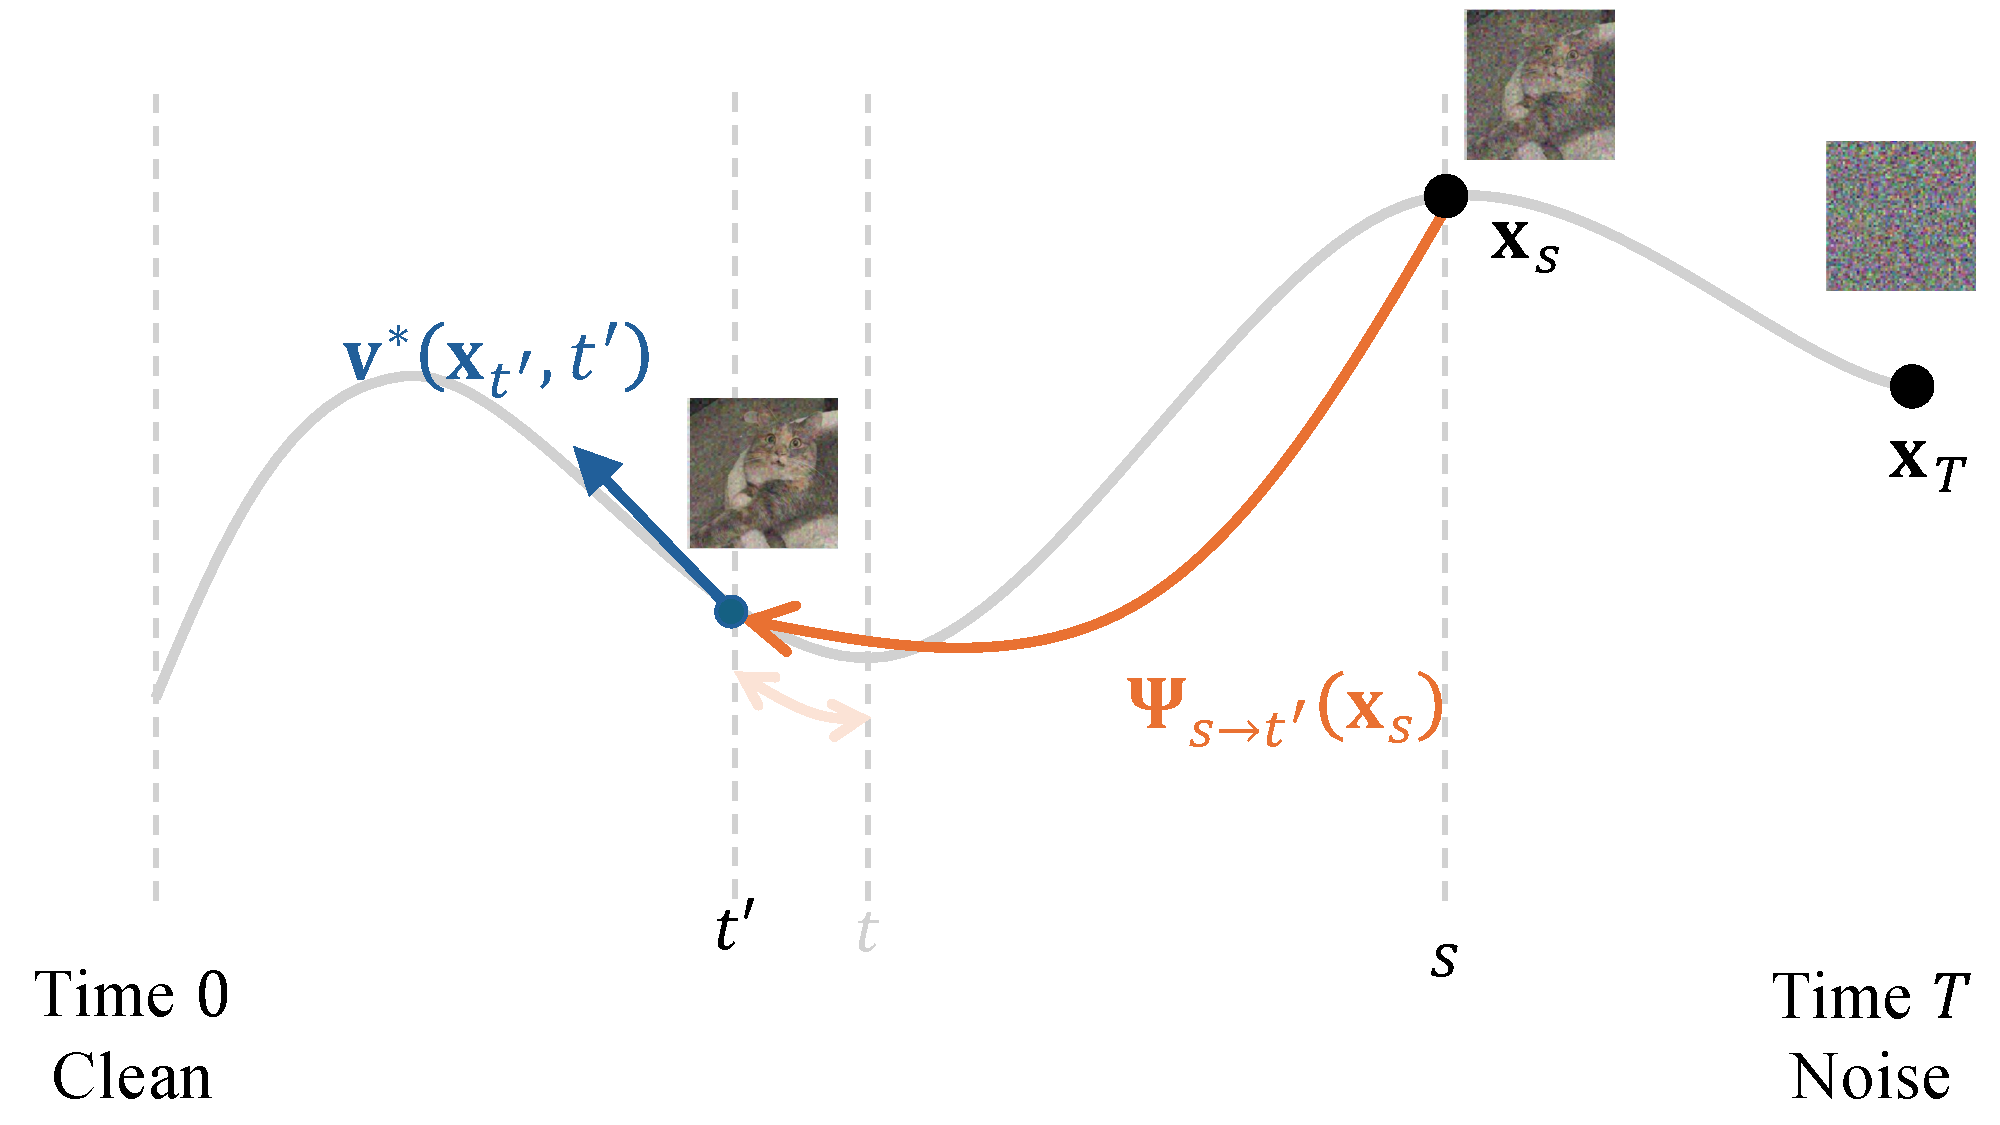
\includegraphics[width=\linewidth]{Images/PartD/lagrangian-2.pdf}
        \caption{Moved ending time $t'$.}
        \label{fig:lagrangian-moved}
    \end{subfigure}

    \caption{\textbfs{Lagrangian consistency of flow maps.}
    The starting state--time pair $(\rvx_s,s)$ is fixed, and the ending time is moved from $t$ to
    $t'$. The output of the flow map moves along the same PF-ODE trajectory, and
    its infinitesimal change equals the ODE velocity:
    $\partial_t \bPsi_{s\to t}(\rvx_s)
    = \rvv^*(\bPsi_{s\to t}(\rvx_s),t)$.}
    \figcredit{Adapted from \citet{dieleman2026flowmaps}.}
    \label{fig:lagrangian-consistency}
\end{figure}

\paragraph{Lagrangian View: Move the Ending Point.}
Fix the starting state--time pair $(\rvx_s,s)$ and vary the ending time
$t$. The ending point then moves along the same trajectory:
\[
\partial_t \bPsi_{s\to t}(\rvx_s)
=
\rvv^*(\bPsi_{s\to t}(\rvx_s),t).
\]
The name ``Lagrangian'' follows the classical particle viewpoint: we
track the ending point along the trajectory as the ending time changes.
Infinitesimally, the ending point moves with the local ODE velocity
evaluated at that point.

\paragraph{Eulerian View: Move the Starting Point.}
Fix the ending time $t$ and slide the starting point along the same trajectory.
The ending point at time $t$ remains fixed:
\[
\frac{\diff}{\diff s}\bPsi_{s\to t}(\rvx_s)=0.
\]
Since $\frac{\diff}{\diff s}\rvx_s=\rvv^*(\rvx_s,s)$, the chain rule gives
\[
\partial_s\bPsi_{s\to t}(\rvx_s)
+
\big(\partial_{\rvx}\bPsi_{s\to t}\big)(\rvx_s)\rvv^*(\rvx_s,s)
=
0.
\]
The term ``Eulerian'' invokes the classical field-based viewpoint: Here, the ending time $t$
is fixed, while the starting state--time pair $(\rvx_s,s)$ moves along the
same ODE trajectory; the ending point at time $t$ therefore remains unchanged. For CM, the ending time is fixed at $t=0$, so the ending point is the clean sample:
\[
    \rvf^*(\rvx_s,s)=\bPsi_{s\to0}(\rvx_s).
\]
Thus, \Cref{eq:conti-ct-motivation} is the starting-time consistency condition
for the special flow map studied in \Cref{sec:discrete-cm,sec:conti-cm}.



This view also recaps the relationship between CTM and MF from
\Cref{subsec:equivalence-ctm-mf}.  Both approximate the same path integral
\[
\bPsi_{s\to t}(\rvx_s)
=
\rvx_s+\int_s^t\rvv^*(\rvx_\tau,\tau)\,\diff\tau,
\]
but expose different trainable surrogates.  CTM represents the ending point through a displacement-style
parameterization, while MF represents the same ending point through the
average drift
\[
\rvh^*(\rvx_s,s,t)
=
\frac{1}{t-s}\int_s^t\rvv^*(\rvx_\tau,\tau)\,\diff\tau.
\]
Substituting
\[
\bPsi_{s\to t}(\rvx_s)=\rvx_s+(t-s)\rvh^*(\rvx_s,s,t)
\]
into the Eulerian starting-time identity yields
\[
\rvh^*(\rvx_s,s,t)
=
\rvv^*(\rvx_s,s)
-
(s-t)
\left[
\partial_s\rvh^*(\rvx_s,s,t)
+
(\partial_{\rvx}\rvh^*)(\rvx_s,s,t)\rvv^*(\rvx_s,s)
\right].
\]
This is the basic Mean Flow identity: the average drift over a long interval is
the instantaneous drift at the starting point, corrected by how the average drift
changes as the starting point slides along the same trajectory.

\begin{figure}[t]
    \centering

    \begin{subfigure}[t]{0.485\textwidth}
        \centering
        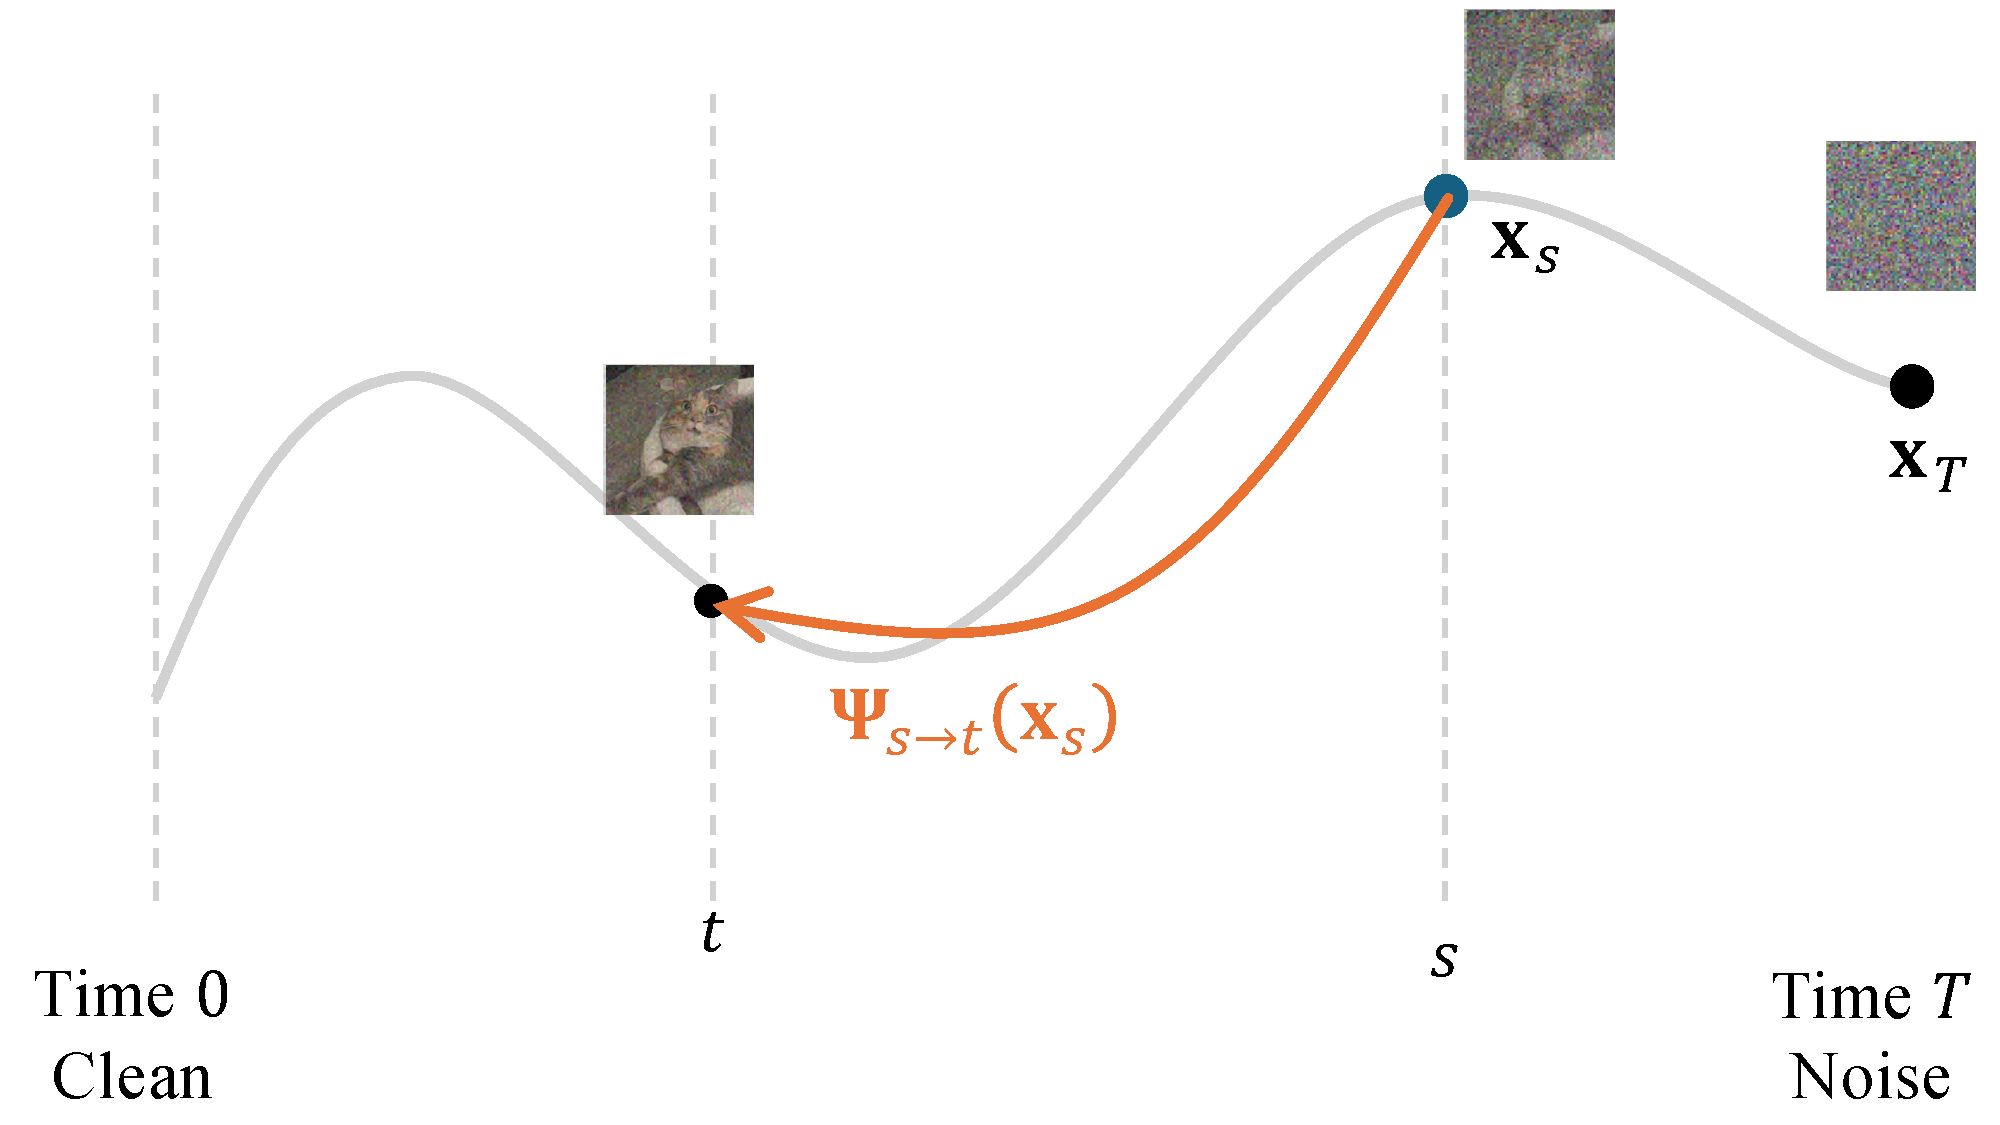
\includegraphics[width=\linewidth]{Images/PartD/eulerian-1.pdf}
        \caption{Base starting time $s$.}
        \label{fig:eulerian-base}
    \end{subfigure}
    \hfill
    \begin{subfigure}[t]{0.485\textwidth}
        \centering
        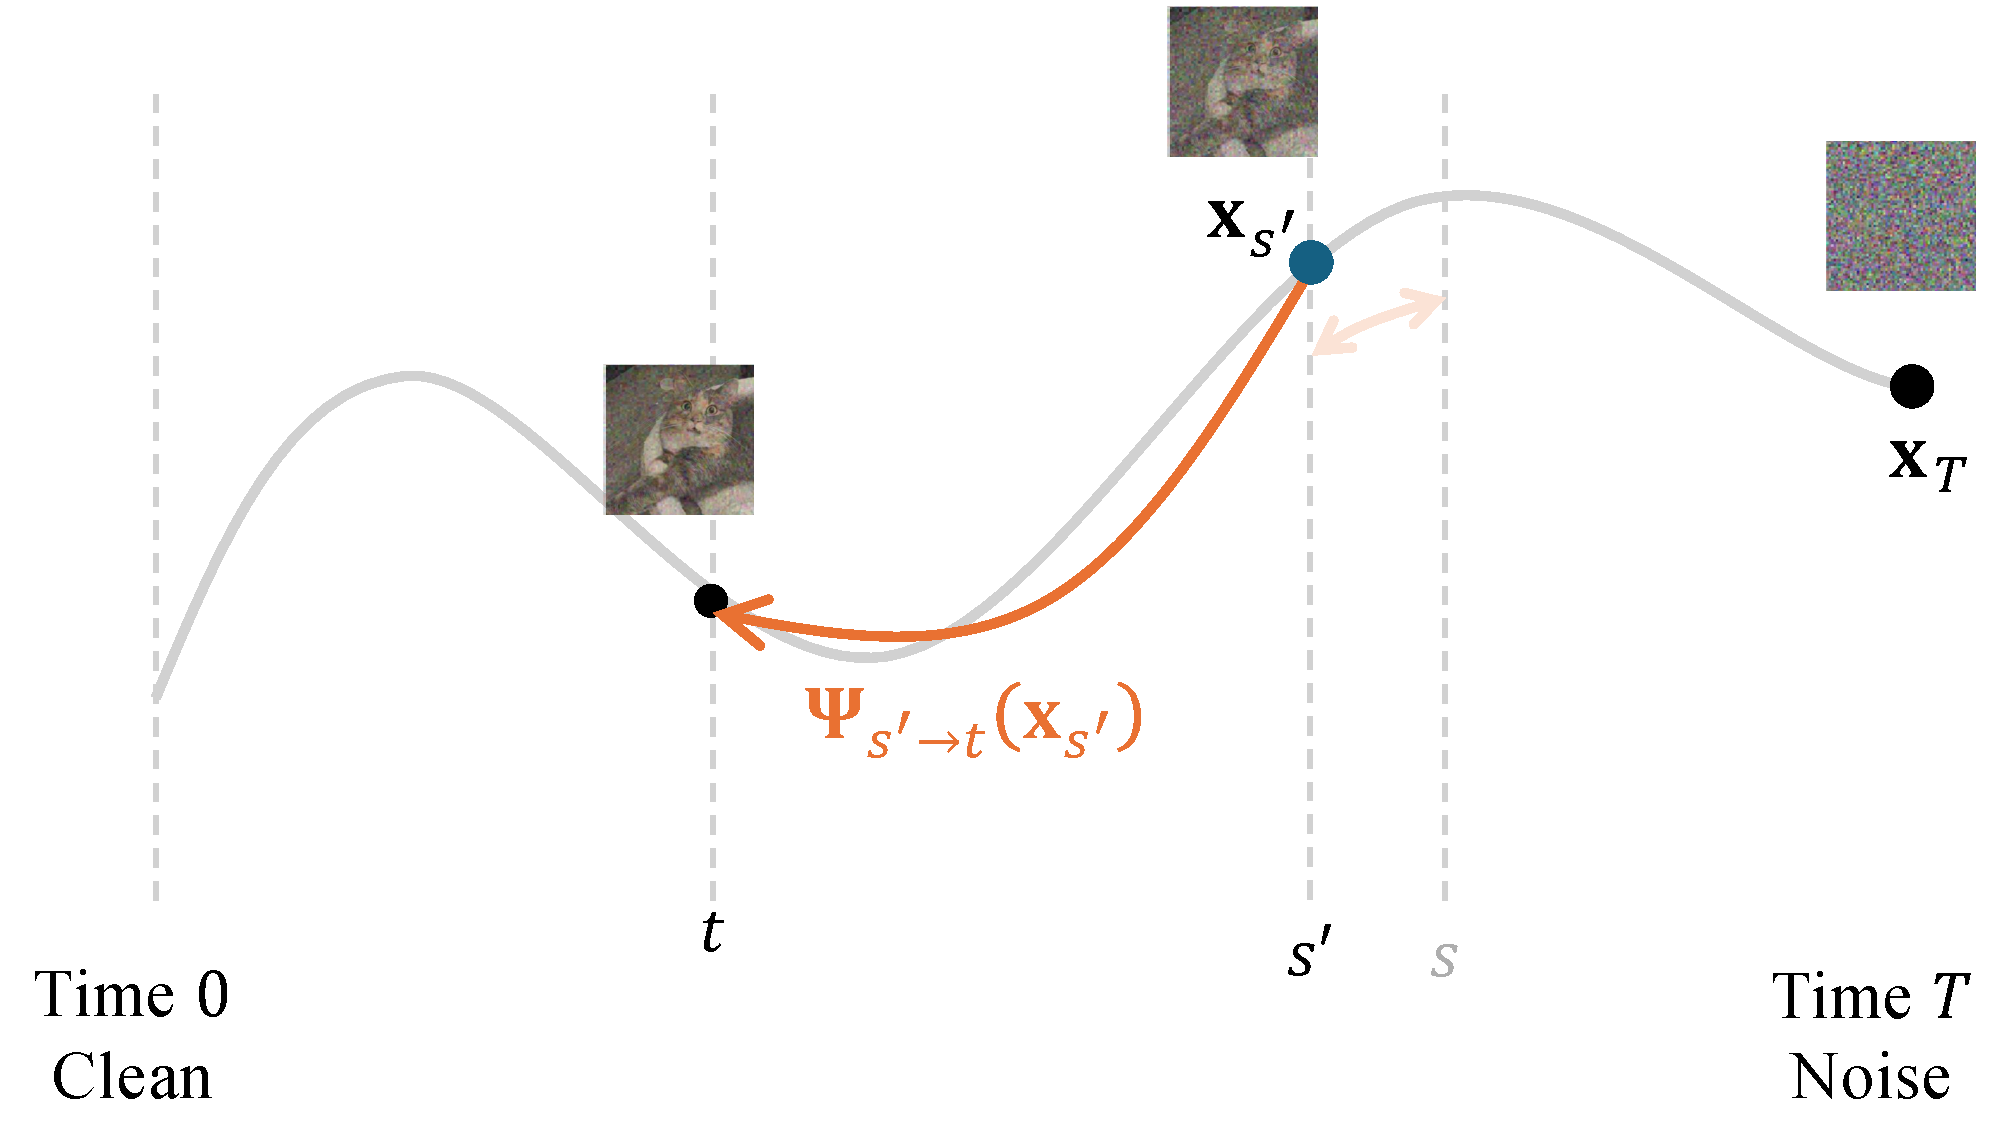
\includegraphics[width=\linewidth]{Images/PartD/eulerian-2.pdf}
        \caption{Moved starting time $s'$.}
        \label{fig:eulerian-moved}
    \end{subfigure}

    \caption{\textbfs{Eulerian consistency of flow maps.}
    The ending time $t$ is fixed, while the starting time is moved from $s$ to
    $s'$. Since the corresponding starting points lie on the same PF-ODE
trajectory, the ending point remains unchanged:
    $\bPsi_{s\to t}(\rvx_s)=\bPsi_{s'\to t}(\rvx_{s'})$.
    Infinitesimally, this gives
    $\frac{\diff}{\diff s}\bPsi_{s\to t}(\rvx_s)=0$, or equivalently
    $\partial_s\bPsi_{s\to t}(\rvx_s)
    +(\partial_{\rvx}\bPsi_{s\to t})(\rvx_s)\rvv^*(\rvx_s,s)=0$.}
        \figcredit{Adapted from \citet{dieleman2026flowmaps}.}
    \label{fig:eulerian-consistency}
\end{figure}

\paragraph{Mathematical Equivalence of the Three Perspectives.}
For an exact ODE flow, the semigroup, Lagrangian, and Eulerian identities
all express the same simple principle: under standard existence,
uniqueness, and smoothness assumptions, an ODE determines a unique
trajectory through each state--time pair. That is, once a state at a
given time is fixed, there is only one path to follow. The semigroup view
splits this path into consecutive pieces, the Lagrangian view follows its
ending point as the ending time changes, and the Eulerian view moves the
starting point along the same path while keeping the ending point fixed.
Thus, the three identities are equivalent descriptions of the same ODE
flow~\citep{arnold1988geometrical,chorin1993mathematical}. Their
connection becomes especially clear by viewing the semigroup identity as
the finite-interval statement, and the Lagrangian and Eulerian identities
as its two infinitesimal forms, obtained by shrinking a short interval near the ending time or near the
starting time, respectively.

The semigroup identity gives the finite-interval form of this principle:
\[
    \bPsi_{u\to t}\big(\bPsi_{s\to u}(\rvx_s)\big)
    =
    \bPsi_{s\to t}(\rvx_s),
    \qquad
    \bPsi_{s\to s}=\rmI .
\]
The two differential views are obtained by shrinking one of the two intervals.

\subparagraph{Ending-Time Limit: the Lagrangian Identity.}
Fix the starting state--time pair $(\rvx_s,s)$ and shrink the final
segment of the trip. For $\Delta t>0$,
\[
    \bPsi_{t\to t-\Delta t}
    \big(\bPsi_{s\to t}(\rvx_s)\big)
    =
    \bPsi_{s\to t-\Delta t}(\rvx_s).
\]
Let $\rvx_t:=\bPsi_{s\to t}(\rvx_s)$.  A first-order expansion of the short
flow gives
\[
    \bPsi_{t\to t-\Delta t}(\rvx_t)
    =
    \rvx_t-\Delta t\,\rvv^*(\rvx_t,t)
    +\mathcal{O}\big((\Delta t)^2\big).
\]
Therefore,
\[
    \frac{
    \bPsi_{s\to t-\Delta t}(\rvx_s)
    -
    \bPsi_{s\to t}(\rvx_s)}
    {-\Delta t}
    =
    \rvv^*(\rvx_t,t)
    +\mathcal{O}(\Delta t).
\]
Taking $\Delta t\to0$ yields the Lagrangian identity
\[
    \partial_t\bPsi_{s\to t}(\rvx_s)
    =
    \rvv^*\big(\bPsi_{s\to t}(\rvx_s),t\big).
\]
Thus, when the starting state--time pair $(\rvx_s,s)$ is fixed and the
ending time changes, the ending point moves with the ODE velocity
evaluated at that point.

\subparagraph{Starting-Time Limit: the Eulerian Identity.} Now fix the ending time $t$ and move the starting state--time pair
backward by a short interval $\Delta s>0$ along the same trajectory:
\[
    \rvx_{s-\Delta s}
    :=
    \bPsi_{s\to s-\Delta s}(\rvx_s)
    =
    \rvx_s-\Delta s\,\rvv^*(\rvx_s,s)
    +\mathcal{O}\big((\Delta s)^2\big).
\]
The semigroup identity gives
\[
    \bPsi_{s-\Delta s\to t}(\rvx_{s-\Delta s})
    =
    \bPsi_{s\to t}(\rvx_s).
\]
Expanding the left-hand side in both the starting state and the starting time gives
\[
    \bPsi_{s-\Delta s\to t}(\rvx_{s-\Delta s})
    =
    \bPsi_{s\to t}(\rvx_s)
    -
    \Delta s\,
    \big(\partial_{\rvx}\bPsi_{s\to t}\big)(\rvx_s)\rvv^*(\rvx_s,s)
    -
    \Delta s\,
    \partial_s\bPsi_{s\to t}(\rvx_s)
    +
    \mathcal{O}\big((\Delta s)^2\big).
\]
Comparing with the semigroup identity and dividing by $-\Delta s$ gives
\[
    \partial_s\bPsi_{s\to t}(\rvx_s)
    +
    \big(\partial_{\rvx}\bPsi_{s\to t}\big)(\rvx_s)\rvv^*(\rvx_s,s)
    =
    \mathcal{O}(\Delta s).
\]
Taking $\Delta s\to0$ yields the Eulerian identity
\[
    \partial_s\bPsi_{s\to t}(\rvx_s)
    +
    \big(\partial_{\rvx}\bPsi_{s\to t}\big)(\rvx_s)\rvv^*(\rvx_s,s)
    =
    0.
\]
Here, the ending time $t$ is fixed, while the starting state--time pair
moves along the same trajectory. The ending point therefore remains
unchanged.

\subparagraph{Recovering the Flow Map from Either Differential Identity.}
Conversely, either differential identity
together with the boundary condition $\bPsi_{s\to s}=\rmI$ recovers the same
flow map.  The Lagrangian identity evolves the ending point from
$\bPsi_{s\to s}(\rvx_s)=\rvx_s$.  The Eulerian identity says that
$\bPsi_{\tau\to t}(\rvx_\tau)$ is constant along the characteristic
$\rvx_\tau=\bPsi_{s\to \tau}(\rvx_s)$, hence
\[
    \bPsi_{s\to t}(\rvx_s)
    =
    \bPsi_{t\to t}(\rvx_t)
    =
    \rvx_t.
\]
Although these perspectives are equivalent at the oracle level, they lead to
different practical algorithms once approximations are introduced: one must
choose which identity to enforce, where to place stop-gradient targets, how to
sample time pairs, and how to parameterize the map.


\paragraph{Closing.}
The central shift explored in this chapter is from learning a local velocity
field to learning finite pieces of its ODE solution map. A conventional
diffusion sampler repeatedly evaluates the local field and numerically
integrates it. A flow-map model instead amortizes part of this integration
during training, so that a long interval can be traversed with one or a few
network evaluations.

This creates a direct route to fast generation, but moves difficulty from
sampling into learning. The model must approximate a more global object, and
its success depends on the parameterization of the map, the construction of
tractable targets, the sampling and weighting of time pairs, and the
stabilization of optimization.

Viewed in this way, flow-map learning is not a new dynamical concept but a
modern learning strategy built around a classical one. It preserves the
trajectory-based foundation of diffusion models while enlarging the design
space for efficient generation. The objective is no longer only to integrate
the generative ODE more efficiently at inference time, but to learn useful
finite-time transitions of its solution map directly.



% \section{Closing Remarks}\label{sec:ch11_cr}

% This final chapter has brought our exploration full circle, culminating in a new paradigm for generative modeling: learning fast, few-step generators from scratch. Moving beyond the approaches of improving numerical solvers or distilling pre-trained models, we have focused on designing standalone training principles that are both principled and highly efficient by design.

% The core innovation presented here is the direct learning of the flow map ($\bm{\Psi}_{s\rightarrow t}$) of the underlying probability flow ODE. The key to making this tractable without a teacher was leveraging the fundamental semi-group property of the ODE flow. This property, which dictates that a long trajectory can be decomposed into shorter segments, provides a powerful self-supervisory signal for training.

% We began with Consistency Models (CMs), which pioneered this approach by learning the special flow map that transports any noisy state back to its clean origin ($\bm{\Psi}_{s\rightarrow 0}$). We then saw this idea generalized by Consistency Trajectory Models (CTM) and Mean Flow (MF), which learn the complete, anytime-to-anytime flow map $\bm{\Psi}_{s\rightarrow t}$ for all $s,t$ satisfying $s\ge t$. While appearing different in their parameterization, we showed that these methods are fundamentally equivalent ways of approximating the same path integral that defines the flow map.

% These flow map models represent a powerful synthesis of the principles developed throughout this book. They inherit the continuous-time foundation of the Score SDE framework and the deterministic transport view of Flow Matching, but reformulate the training objective to be self-contained and efficient.

% By learning the solution map directly, these standalone models successfully unite the high sample quality of iterative diffusion processes with the inference speed of one-step generators. They resolve the fundamental trade-off between fidelity and speed, marking a significant milestone in generative modeling. This achievement represents not an end, but the beginning of a new chapter in the design of powerful, efficient, and controllable generative AI.



% Diffusion models may at first appear as a collection of many acronyms and variants, yet their underlying idea is remarkably simple. At a high level, they provide mechanisms for \emph{transporting probability mass} from a simple reference distribution, such as Gaussian noise, to a complex data distribution over time. From this perspective, generation can be viewed as the evolution of a \emph{cloud of particles}, and the mathematical structure becomes much less mysterious: it is fundamentally a problem of \emph{time-dependent change of variables}. In continuous time, deterministic motion of particles leads to the continuity equation, while motion with additional random perturbation leads to the Fokker-Planck equation. Many seemingly different formulations can be understood as variations built on this common foundation.

% At the same time, the classical strength of diffusion models, namely their ability to generate \emph{high-fidelity} samples, is closely tied to a classical weakness: \emph{iterative sampling}. When the reverse dynamics must be integrated through many small steps, generation remains computationally slow. Flow map models extend the same basic viewpoint in a natural direction. Rather than learning only infinitesimal updates and then numerically integrating them, they seek to learn the \emph{time-jump maps} of the probability-flow ODE (PF-ODE) directly. That is, they aim to approximate the flow map
% \[
% \Psi_{s\to t},
% \]
% so that a long chain of small updates may be replaced by a small number of large but accurate transitions. Consistency Models (CM), Consistency Trajectory Models (CTM), and Mean Flow (MF) provide three concrete examples of this idea. Each imposes a different structural principle on the flow map, such as consistency, semigroup structure, or mean-slope identities, in order to construct practical training targets when the exact flow map is unavailable.

% Stepping back, the main message is encouraging. Diffusion is not merely a single method, but a \emph{general principle for constructing generators} from a prescribed forward process. Once we adopt the viewpoint of first choosing a forward corruption mechanism and then learning the corresponding reverse transport, a wide range of designs becomes possible, each balancing \emph{stability}, \emph{sample quality}, and \emph{generation speed} in different ways. Flow map models represent one promising direction, but they are unlikely to be the final answer. The broader opportunity is to preserve the same clean backbone: define a forward transport process, understand how the distribution evolves through change of variables, and then develop new \emph{parameterizations} and \emph{training objectives} that make \emph{fast generation} as reliable as the best step-by-step samplers.


%%%%%%%%%%%%%%%%%%%%%%%%%%%%%%%%%%%%%%%%%%%%%%%%%%%%%%%%%%%%%%%%%%%%%%%%
\clearpage
\newpage
%%%%%%%%%%%%%%%%%%%%%%%%%%%%%%%%%%%%%%%%%%%%%%%%%%%%%%%%%%%%%%%%%%%%%%%%



